\documentclass[compress]{beamer}
\usepackage{ifthen,verbatim,amsmath}

\newcommand{\isnote}{}
\xdefinecolor{lightyellow}{rgb}{1.,1.,0.25}
\xdefinecolor{darkblue}{rgb}{0.1,0.1,0.7}
\xdefinecolor{darkgreen}{rgb}{0.1,0.7,0.1}

%% Uncomment this to get annotations
%% \def\notes{\addtocounter{page}{-1}
%%            \renewcommand{\isnote}{*}
%% 	   \beamertemplateshadingbackground{lightyellow}{white}
%%            \begin{frame}
%%            \frametitle{Notes for the previous page (page \insertpagenumber)}
%%            \itemize}
%% \def\endnotes{\enditemize
%% 	      \end{frame}
%%               \beamertemplateshadingbackground{white}{white}
%%               \renewcommand{\isnote}{}}

%% Uncomment this to not get annotations
\def\notes{\comment}
\def\endnotes{\endcomment}

\setbeamertemplate{navigation symbols}{}
\setbeamertemplate{headline}{\mbox{ } \hfill
\begin{minipage}{5.5 cm}
\vspace{-0.75 cm} \small
\end{minipage} \hfill
\begin{minipage}{4.5 cm}
\vspace{-0.75 cm} \small
\begin{flushright}
\ifthenelse{\equal{\insertpagenumber}{1}}{}{Jim Pivarski \hspace{0.2 cm} \insertpagenumber\isnote/\pageref{numpages}}
\end{flushright}
\end{minipage}\mbox{\hspace{0.2 cm}}\includegraphics[height=1 cm]{../cmslogo} \hspace{0.1 cm} \includegraphics[height=1 cm]{../tamulogo} \hspace{0.01 cm} \vspace{-1.05 cm}}

\begin{document}
\begin{frame}
\vfill
\begin{center}
\textcolor{darkblue}{\Large Proposed alignments for barrel and endcap}

\vfill
\begin{columns}
\column{0.3\linewidth}
\begin{center}
\large
\textcolor{darkblue}{Jim Pivarski}

\vspace{0.2 cm}
Alexei Safonov
\end{center}
\end{columns}

\begin{columns}
\column{0.3\linewidth}
\begin{center}
\scriptsize
{\it Texas A\&M University}
\end{center}
\end{columns}

\vfill
 1 June, 2009

\end{center}
\end{frame}

%% \begin{notes}
%% \item This is the annotated version of my talk.
%% \item If you want the version that I am presenting, download the one
%% labeled ``slides'' on Indico (or just ignore these yellow pages).
%% \item The annotated version is provided for extra detail and a written
%% record of comments that I intend to make orally.
%% \item Yellow notes refer to the content on the {\it previous} page.
%% \item All other slides are identical for the two versions.
%% \end{notes}

\small

\begin{frame}
\frametitle{Outline}
\begin{itemize}\setlength{\itemsep}{0.75 cm}
\item Final studies and validation of the barrel alignment
\item Presentation of the endcap disk alignment
\end{itemize}
%% \hspace{-0.83 cm} \textcolor{darkblue}{\Large Outline2}
\end{frame}

\begin{frame}
\frametitle{Important corrections}

\[ \mbox{Apr 27\hspace{0.3 cm}} \xrightarrow{\mbox{\scriptsize increase $p_T$ cut}} \mbox{\hspace{0.3 cm}May 25\hspace{0.3 cm}} \xrightarrow{\mbox{\scriptsize use final tracker}} \mbox{\hspace{0.3 cm}May 29} \]

\mbox{ } \hfill \begin{minipage}{3.8 cm} \scriptsize twisted barrel about 0.35~mrad \end{minipage} \hfill \begin{minipage}{3.5 cm} \scriptsize translated chambers with $\sigma \sim 2$~mm, no rotations \end{minipage} \hfill \mbox{ }

\vspace{0.35 cm}
\hspace{-0.83 cm} \textcolor{darkblue}{\Large Unimportant corrections}

\begin{itemize}
\item $\vec{B}(\vec{x})$ correction when $100 < p_T < 200$~GeV
\item Using the final tracker APEs, in addition to final tracker alignment:
\end{itemize}

\mbox{ } \hfill 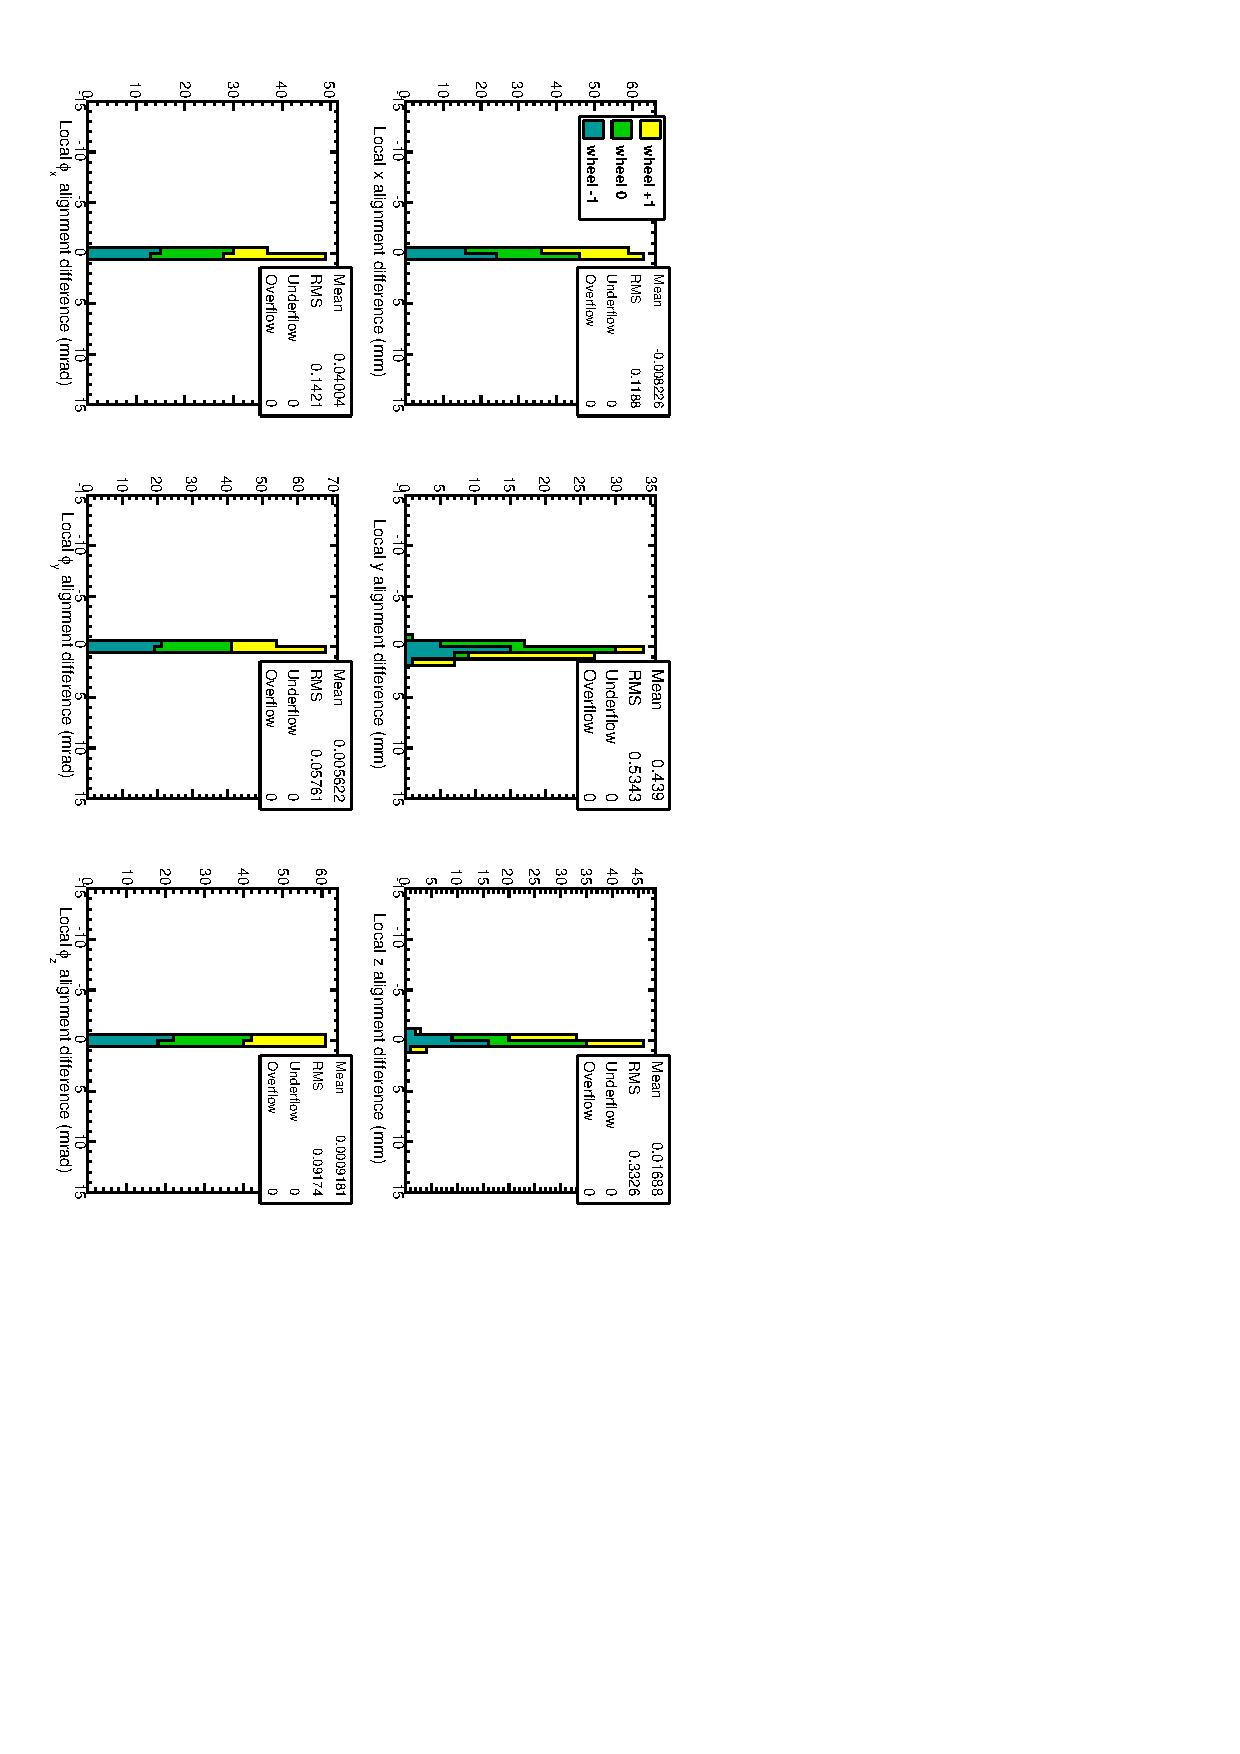
\includegraphics[height=0.75\linewidth, angle=90]{hip_finaltrackerAPEdiff.pdf} \hfill \mbox{ }
\end{frame}

\begin{frame}
\frametitle{Segment extrapolation}

\vspace{0.25 cm}
Difference in angle between station~$A$ and station~$B$, \mbox{measured by segments:\hspace{-1 cm}}

\vspace{0.25 cm}
\textcolor{darkblue}{\mbox{ } \hspace{0.35 cm} May 25 \hspace{2.7 cm} changes in DB \hspace{1.7 cm} May 29? \hspace{0.25 cm} \mbox{ }}

\vspace{0.25 cm}
\mbox{\hspace{-0.75 cm}
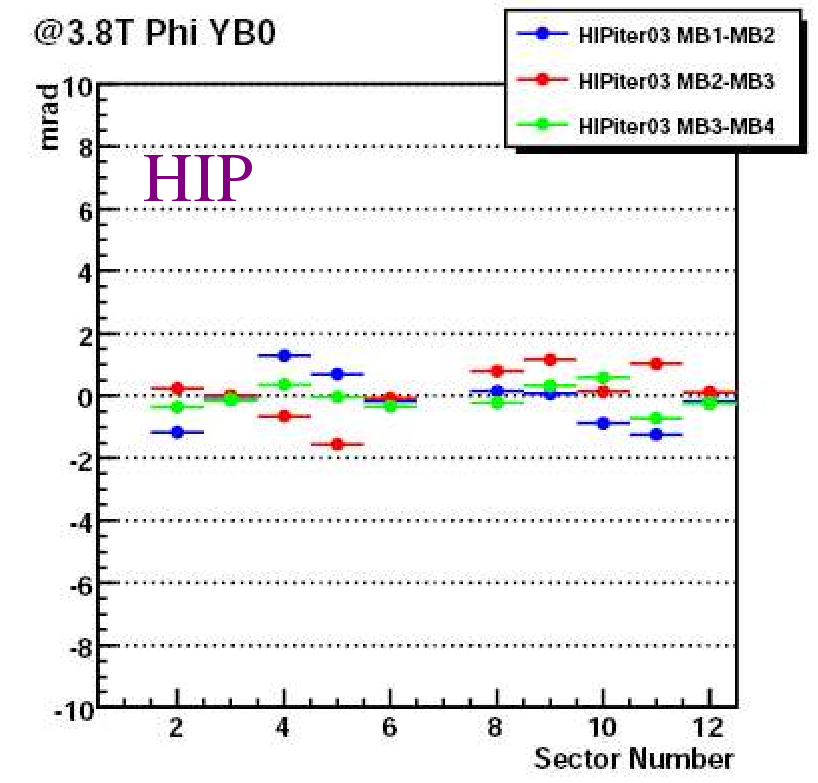
\includegraphics[height=4 cm]{alicia_phiyC.png}
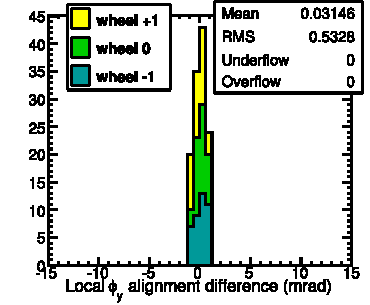
\includegraphics[height=3.5 cm]{hip_tracker_difference_phiy.pdf}
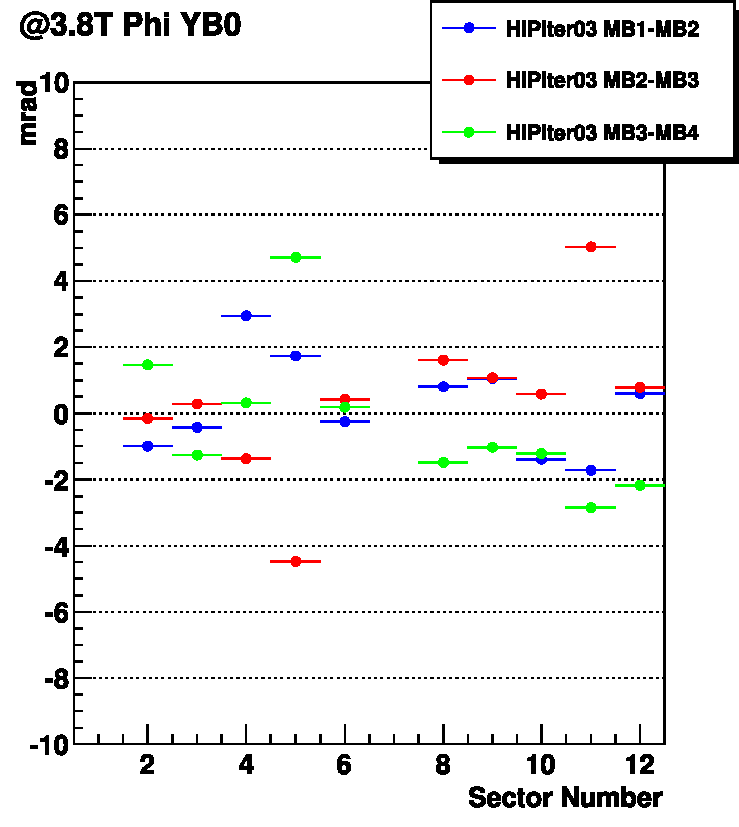
\includegraphics[height=4 cm]{cw0Phi.pdf}}

\hfill \textcolor{darkblue}{\scriptsize A.~Calderon}

\begin{itemize}
\item How can segment differences change by more than 2~mrad when no angle was moved in the DB by more than 1~mrad?
\item Something seems to have gone wrong in this test; possibly configured incorrectly (very short timescale)
\end{itemize}
\end{frame}

\begin{frame}
\frametitle{Backup: local $x$ matching}
\only<1-2>{\begin{itemize}
\item Not admissible because of error observed in $\phi_y$ plots, but
  $x$ plots by themselves do not indicate worse resolution

(previously: 0.8~mm in stations~1--3, 1.6~mm station~4 due to internal structure)
\end{itemize}}
\only<3>{\begin{itemize}
\item The green points on the left (which do have a worse
  resolution) do not appear on the right--- a mis-match within the set of plots?
\end{itemize}}

\only<1>{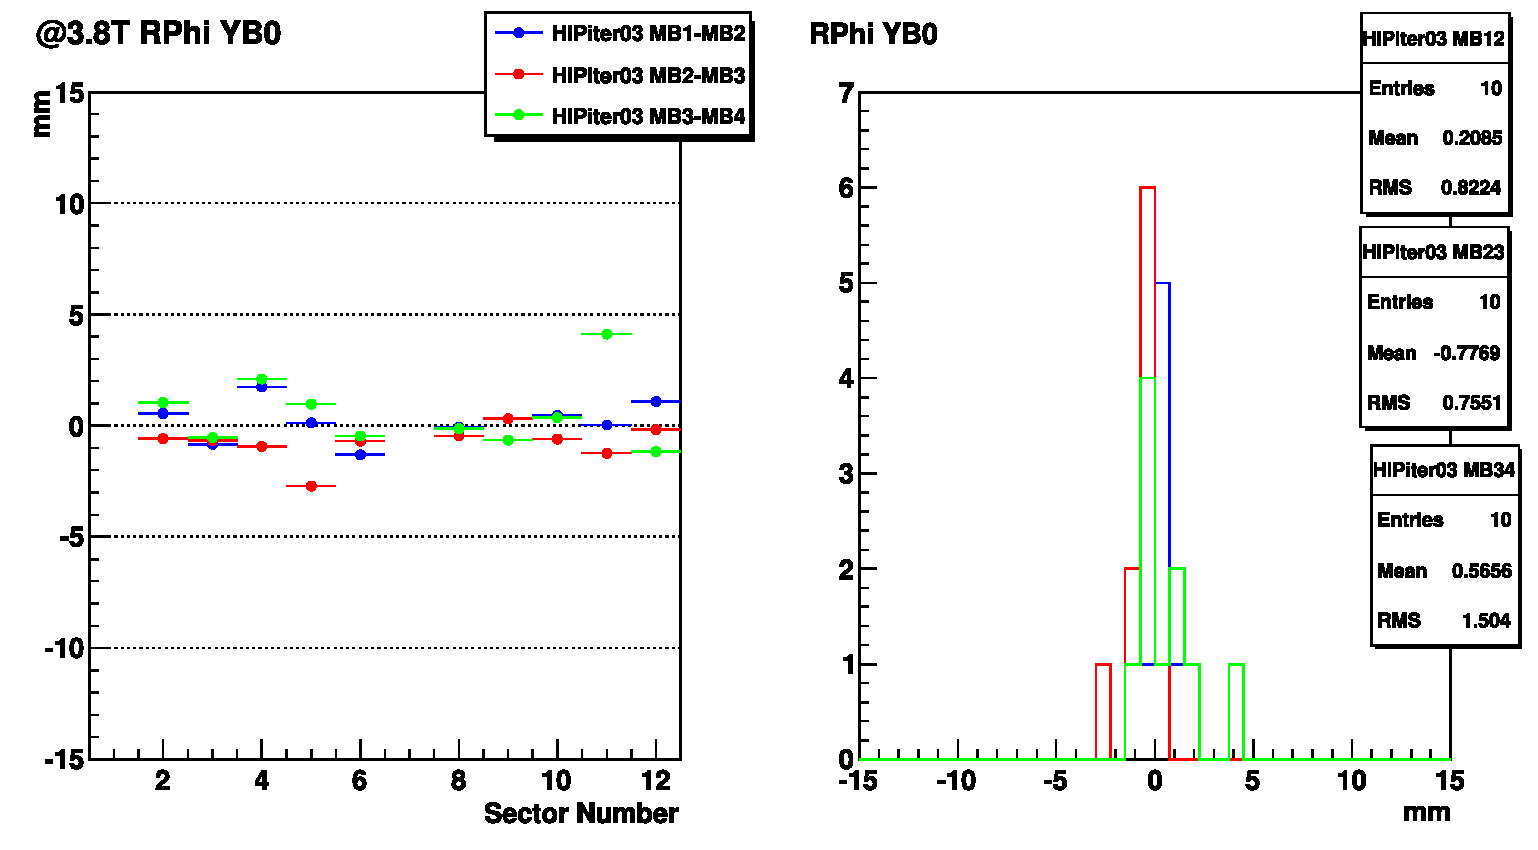
\includegraphics[width=\linewidth]{cw0RPhi.pdf}}\only<2>{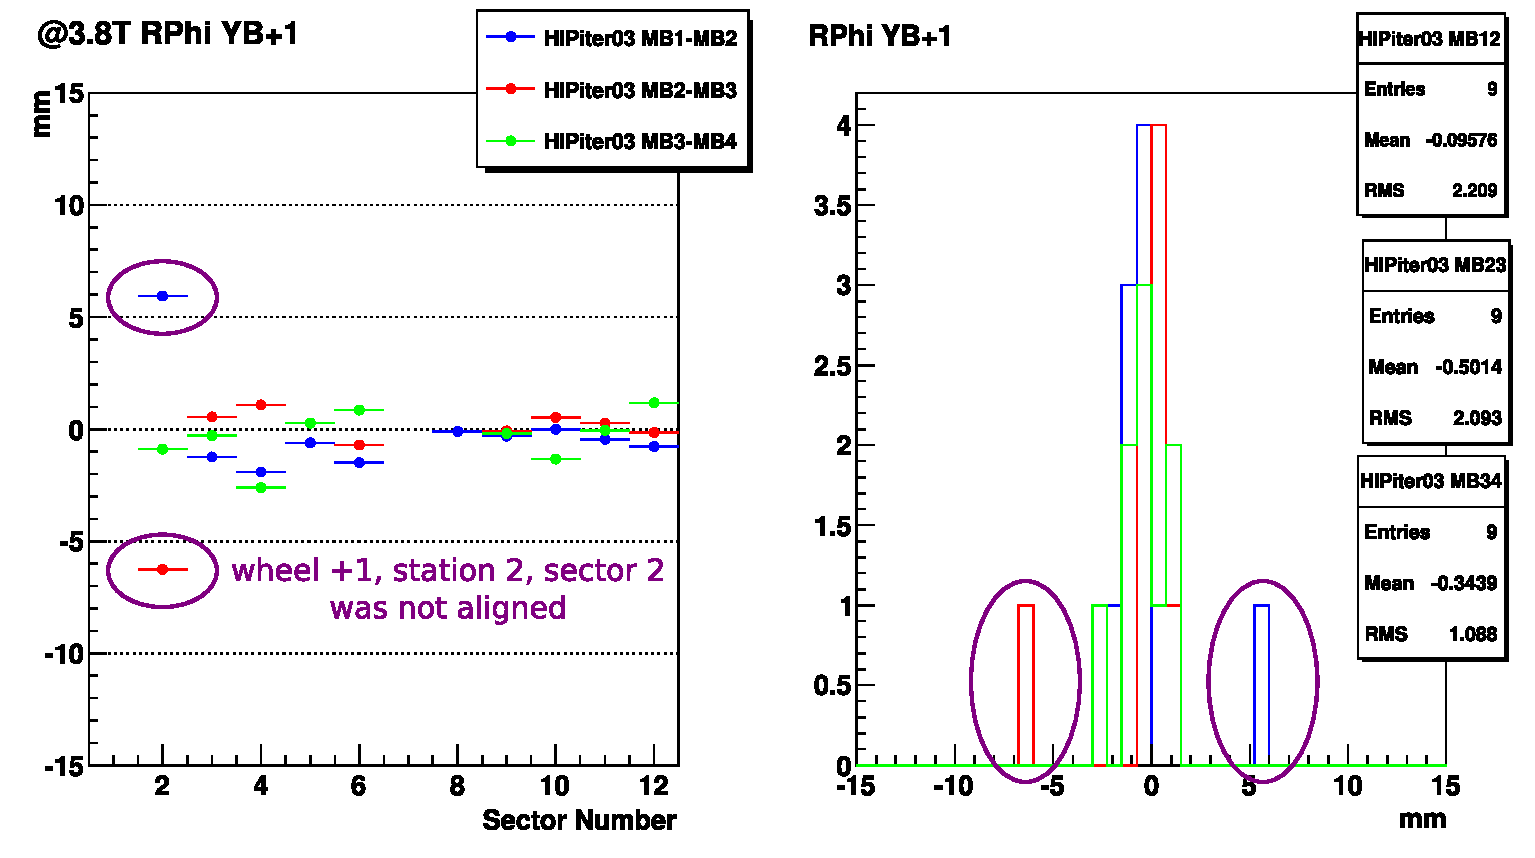
\includegraphics[width=\linewidth]{cw1RPhi.pdf}}\only<3>{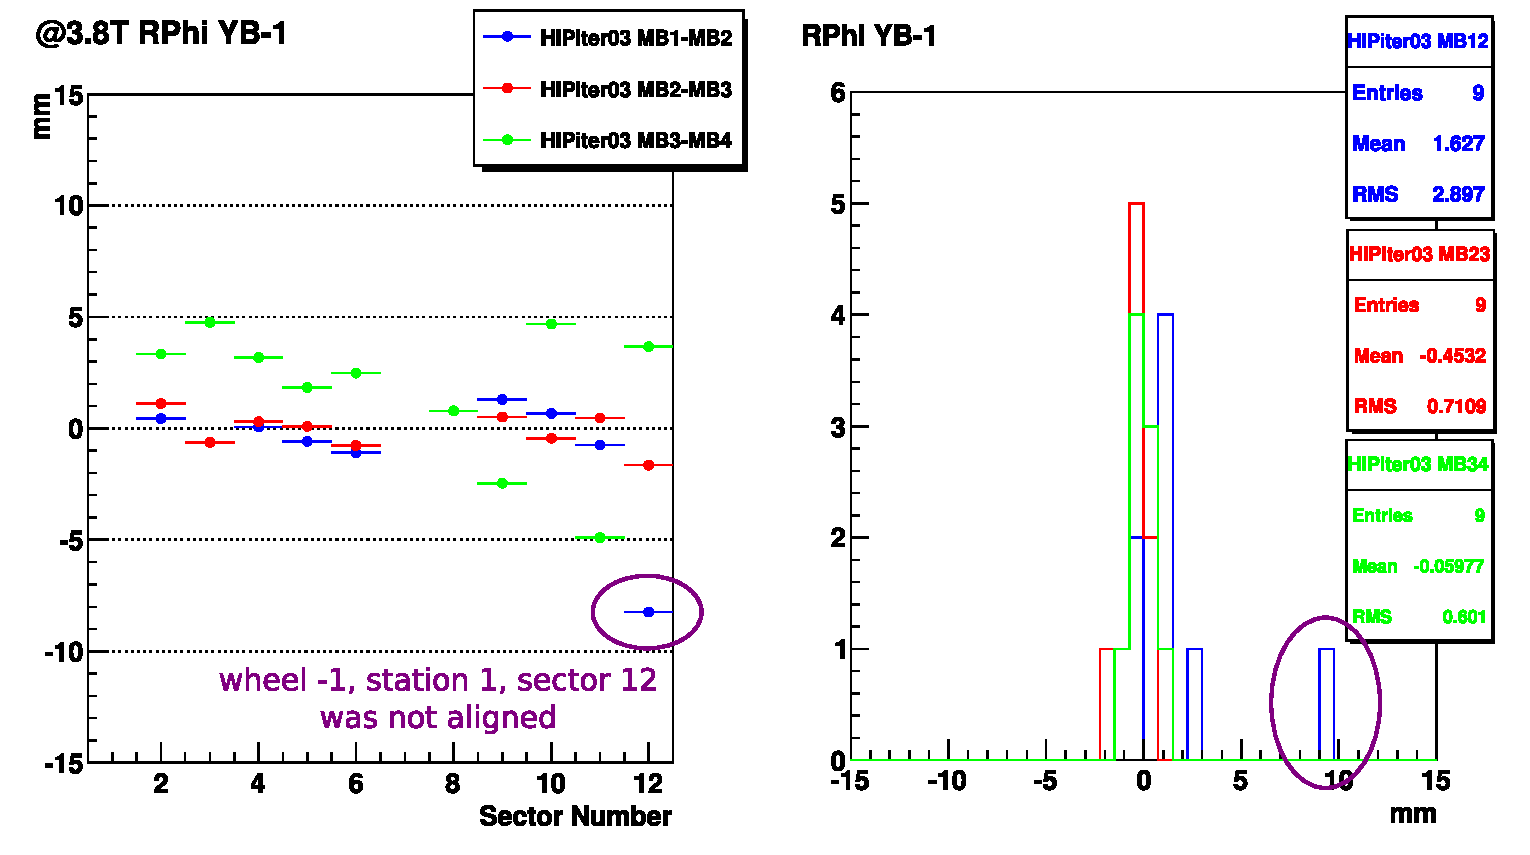
\includegraphics[width=\linewidth]{cwm1RPhi.pdf}}
\end{frame}

\begin{frame}
\frametitle{Cosmic splitting (\only<1>{1}\only<2>{2}\only<3>{3}\only<4>{4}/4)}

\begin{itemize}
\item Sequence of $\frac{\left(1/p_T\right)_{\mbox{\tiny top}} - \left(1/p_T\right)_{\mbox{\tiny bot}}}{\sqrt{2} \, \left(1/p_T\right)_{\mbox{\tiny bot}}}$ (equal to $\frac{\left(p_T\right)_{\mbox{\tiny top}} - \left(p_T\right)_{\mbox{\tiny bot}}}{\sqrt{2} \, \left(p_T\right)_{\mbox{\tiny bot}}}$ if Gaussian)
\item Vertical axis is resolution from 1 to 10\%
\item Key: \textcolor{red}{tracker-only,} sometimes with station~1, \textcolor{darkgreen}{with station~1,} \mbox{\textcolor{blue}{all stations}\hspace{-1 cm}}
\end{itemize}

\mbox{ } \hfill \only<1>{CRAFT\_ALL\_V4 (before global alignment)}\only<2>{CRAFT\_ALL\_V5--12 (early February)}\only<3>{without latest tracker (May 25)}\only<4>{final muon alignment (May 29)} \hfill \mbox{ }

\begin{columns}
\column{0.8\linewidth}
\only<1>{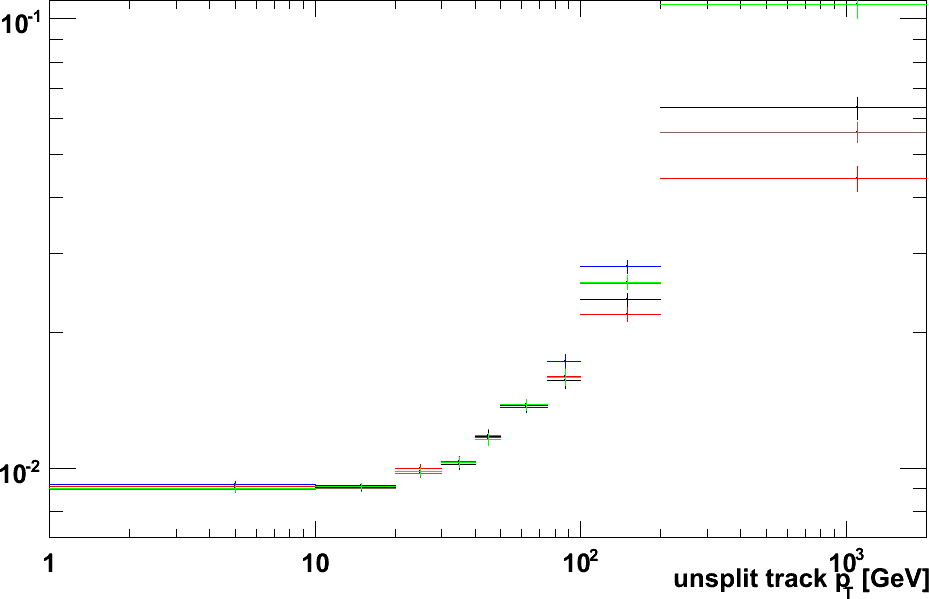
\includegraphics[width=\linewidth]{sigma_inv_pt_relres_6.png}}  % V4
\only<2>{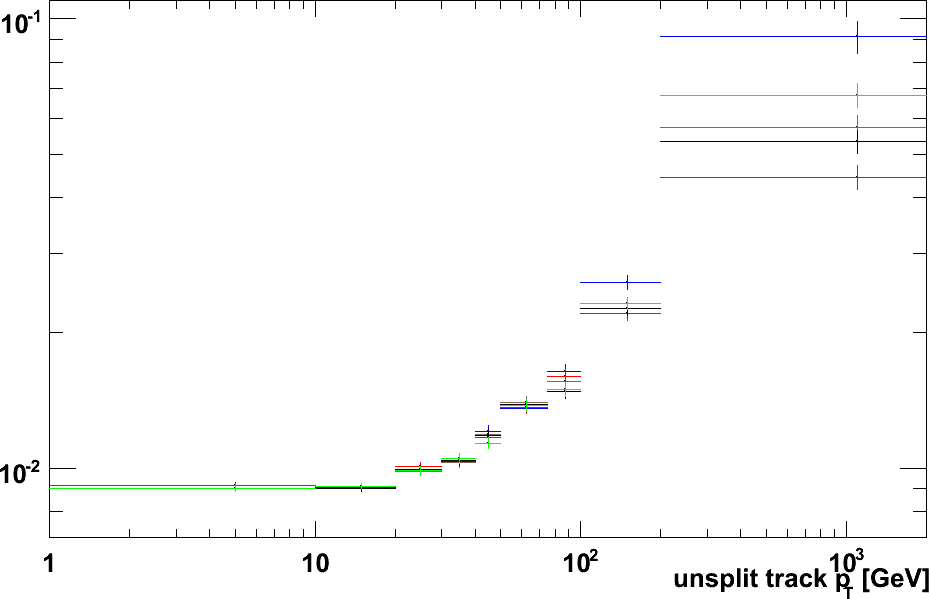
\includegraphics[width=\linewidth]{sigma_inv_pt_relres_7.png}}  % V11
\only<3>{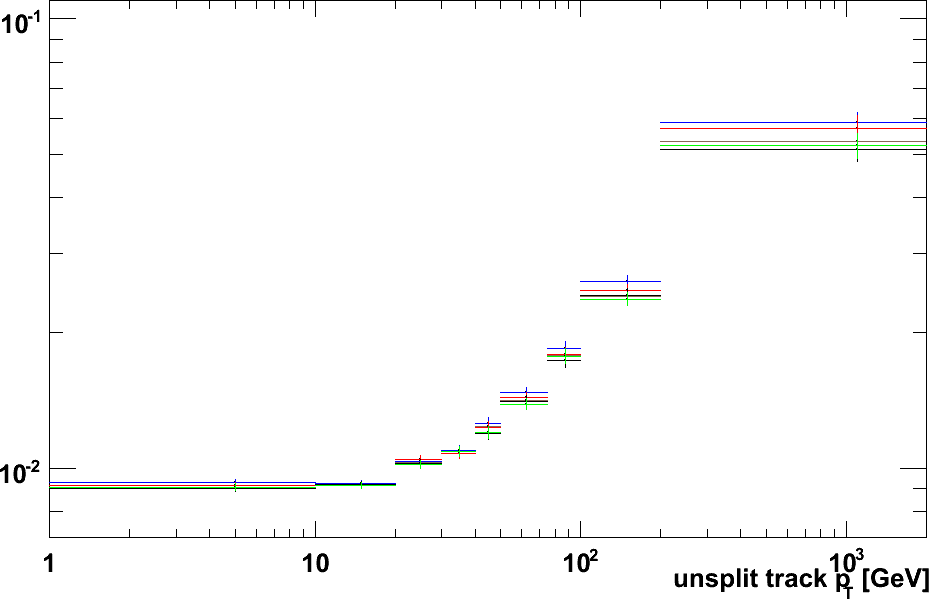
\includegraphics[width=\linewidth]{sigma_inv_pt_relres_1.png}}  % without latest tracker (May 25)
\only<4>{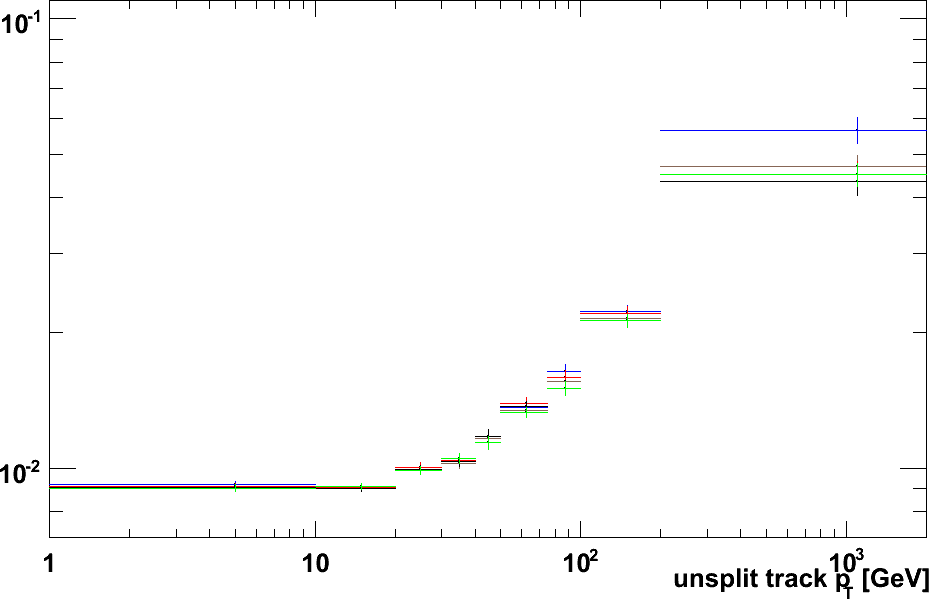
\includegraphics[width=\linewidth]{sigma_inv_pt_relres_4.png}}  % with latest tracker (May 29)
\column{0.2\linewidth}
\begin{minipage}{\linewidth}
\tiny Last bin is always statistically independent of tracks used for alignment
\end{minipage}

\vspace{2 cm}
\textcolor{darkblue}{\scriptsize J.~Tucker}
\end{columns}
\end{frame}

\begin{frame}
\frametitle{Backup: highest bin}
\begin{itemize}
\item Sequence of $\frac{\left(1/p_T\right)_{\mbox{\tiny top}} - \left(1/p_T\right)_{\mbox{\tiny bot}}}{\sqrt{2} \, \left(1/p_T\right)_{\mbox{\tiny bot}}}$ (equal to $\frac{\left(p_T\right)_{\mbox{\tiny top}} - \left(p_T\right)_{\mbox{\tiny bot}}}{\sqrt{2} \, \left(p_T\right)_{\mbox{\tiny bot}}}$ if Gaussian)
\item 200--2000~GeV (these tracks were not used in alignment)
\item Key: \textcolor{red}{tracker-only,} sometimes with station~1, \textcolor{darkgreen}{with station~1,} \mbox{\textcolor{blue}{all stations}\hspace{-1 cm}}
\end{itemize}

\mbox{ } \hfill \only<1>{CRAFT\_ALL\_V4 (before global alignment)}\only<2>{CRAFT\_ALL\_V5--12 (early February)}\only<3>{without latest tracker (May 25)}\only<4>{final muon alignment (May 29)} \hfill \mbox{ }

\begin{columns}
\column{0.8\linewidth}
\only<1>{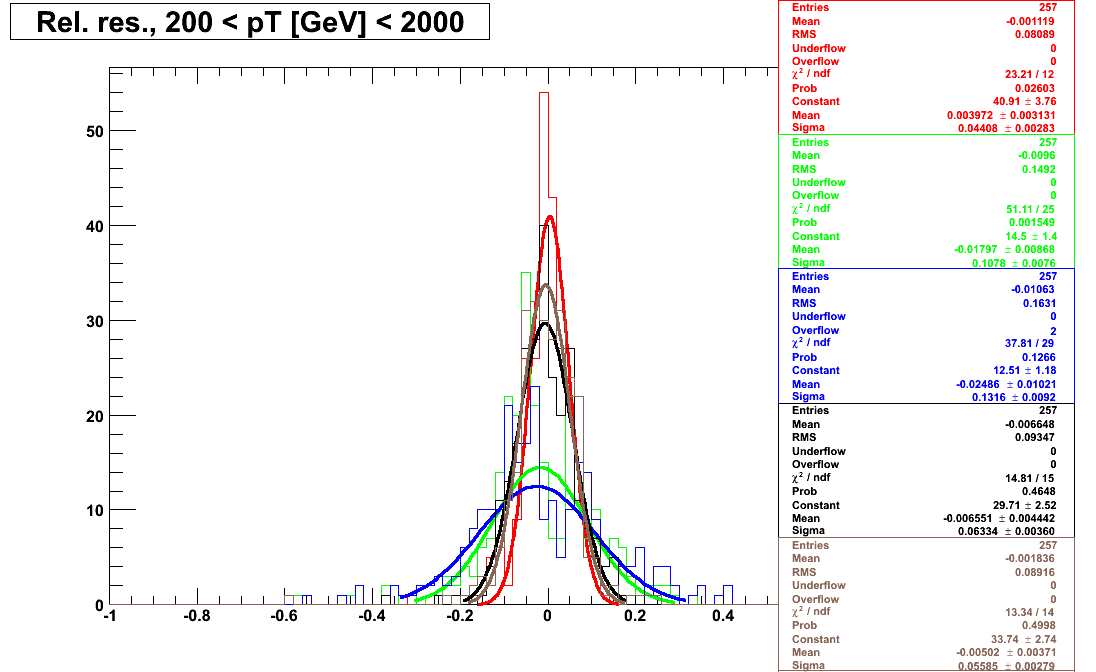
\includegraphics[width=\linewidth]{R1n-pT2002000_6.png}}  % V4
\only<2>{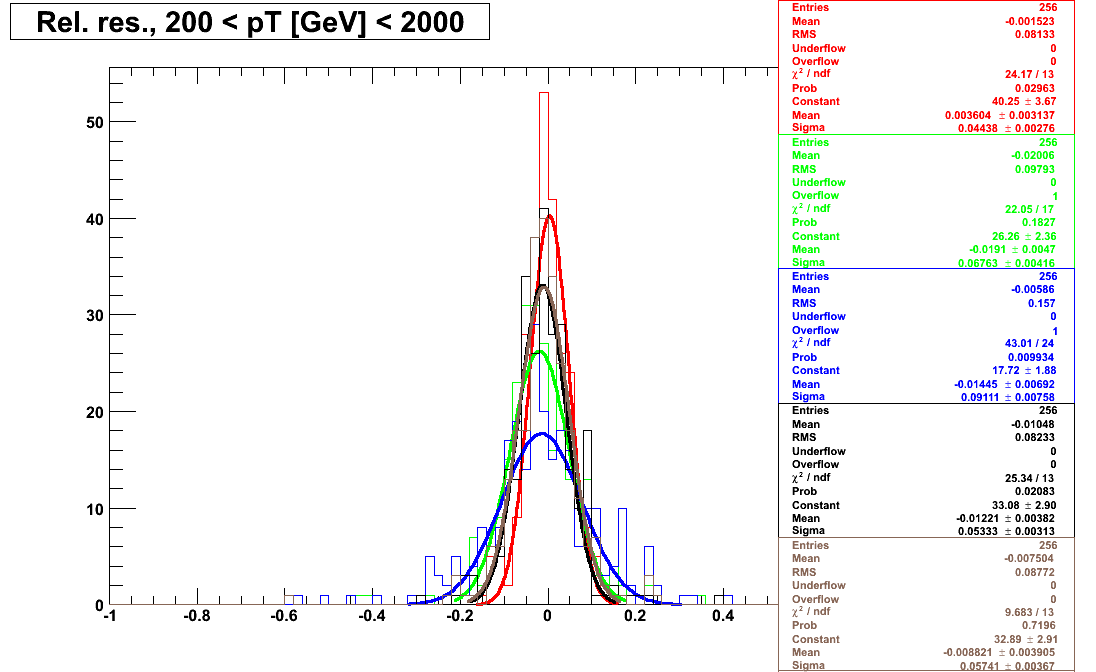
\includegraphics[width=\linewidth]{R1n-pT2002000_7.png}}  % V11
\only<3>{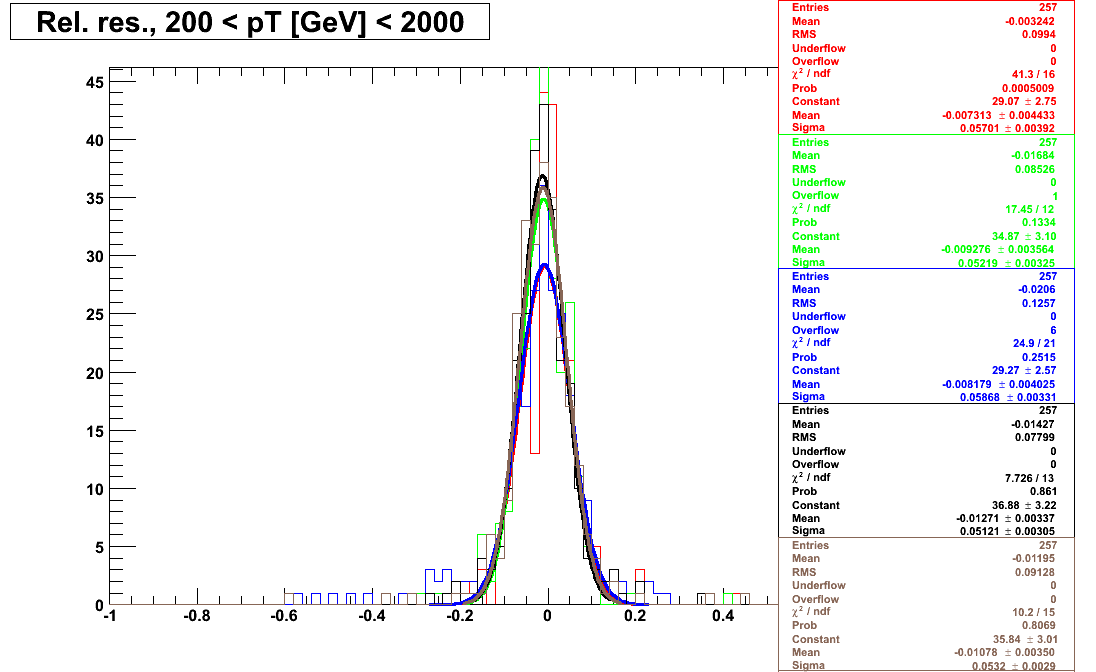
\includegraphics[width=\linewidth]{R1n-pT2002000_1.png}}  % without latest tracker (May 25)
\only<4>{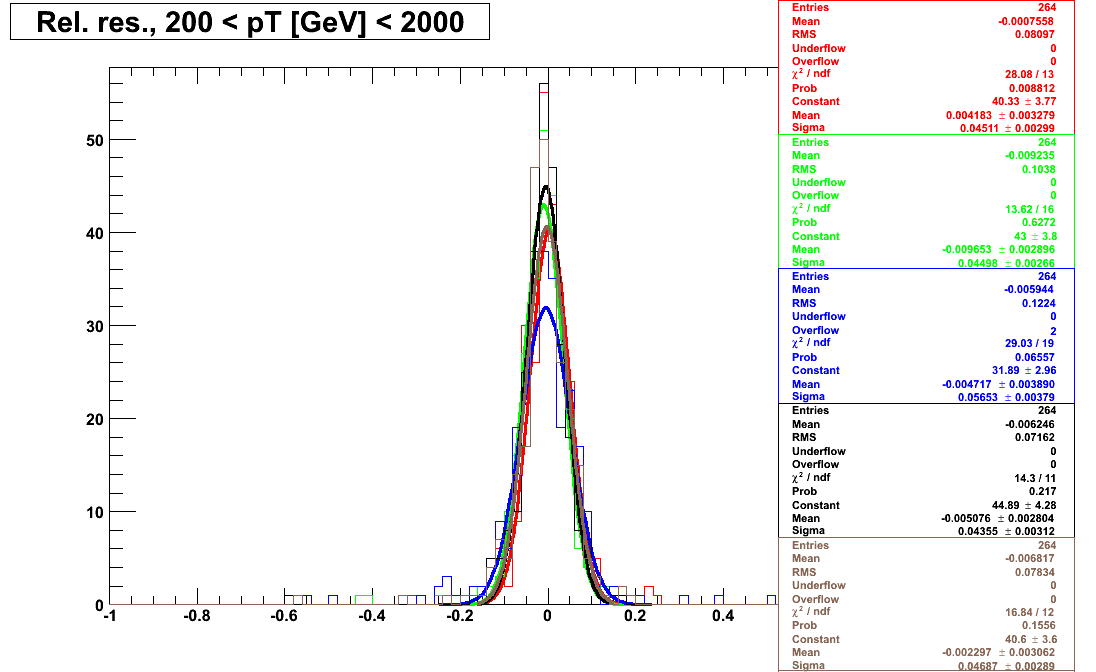
\includegraphics[width=\linewidth]{R1n-pT2002000_4.png}}  % with latest tracker (May 29)
\column{0.2\linewidth}
\mbox{ }

\vspace{4 cm}
\textcolor{darkblue}{\scriptsize J.~Tucker}
\end{columns}
\end{frame}

\begin{frame}
\frametitle{Backup: second-highest bin}
\begin{itemize}
\item Sequence of $\frac{\left(1/p_T\right)_{\mbox{\tiny top}} - \left(1/p_T\right)_{\mbox{\tiny bot}}}{\sqrt{2} \, \left(1/p_T\right)_{\mbox{\tiny bot}}}$ (equal to $\frac{\left(p_T\right)_{\mbox{\tiny top}} - \left(p_T\right)_{\mbox{\tiny bot}}}{\sqrt{2} \, \left(p_T\right)_{\mbox{\tiny bot}}}$ if Gaussian)
\item 100--200~GeV (these tracks were used in the May alignments)
\item Key: \textcolor{red}{tracker-only,} sometimes with station~1, \textcolor{darkgreen}{with station~1,} \mbox{\textcolor{blue}{all stations}\hspace{-1 cm}}
\end{itemize}

\mbox{ } \hfill \only<1>{CRAFT\_ALL\_V4 (before global alignment)}\only<2>{CRAFT\_ALL\_V5--12 (early February)}\only<3>{without latest tracker (May 25)}\only<4>{final muon alignment (May 29)} \hfill \mbox{ }

\begin{columns}
\column{0.8\linewidth}
\only<1>{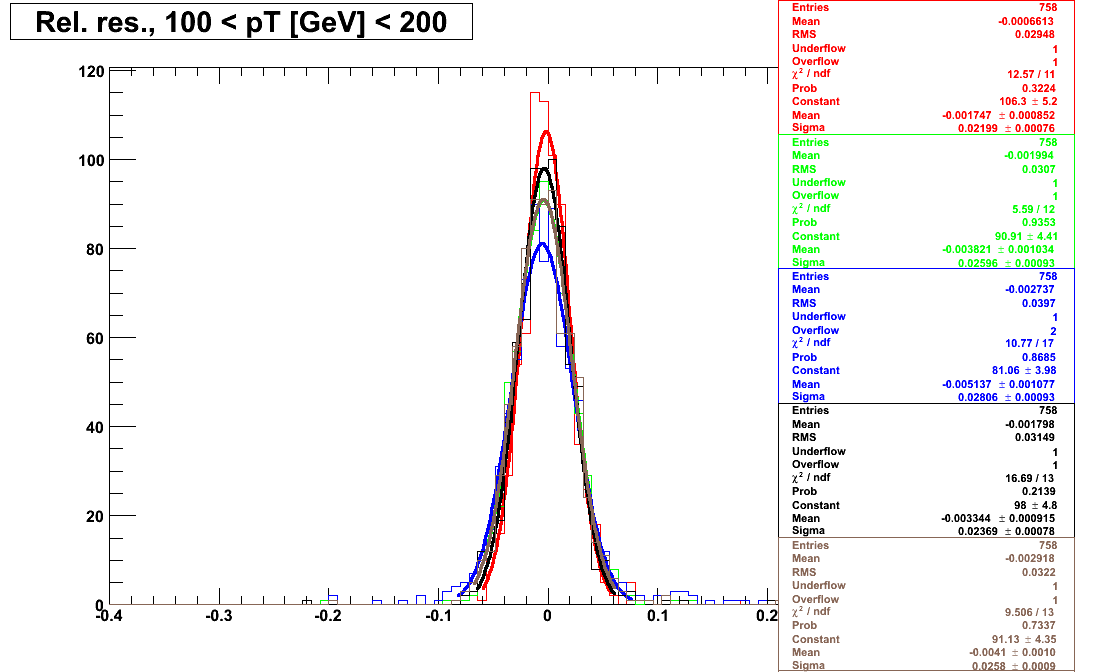
\includegraphics[width=\linewidth]{R1n-pT100200_6.png}}  % V4
\only<2>{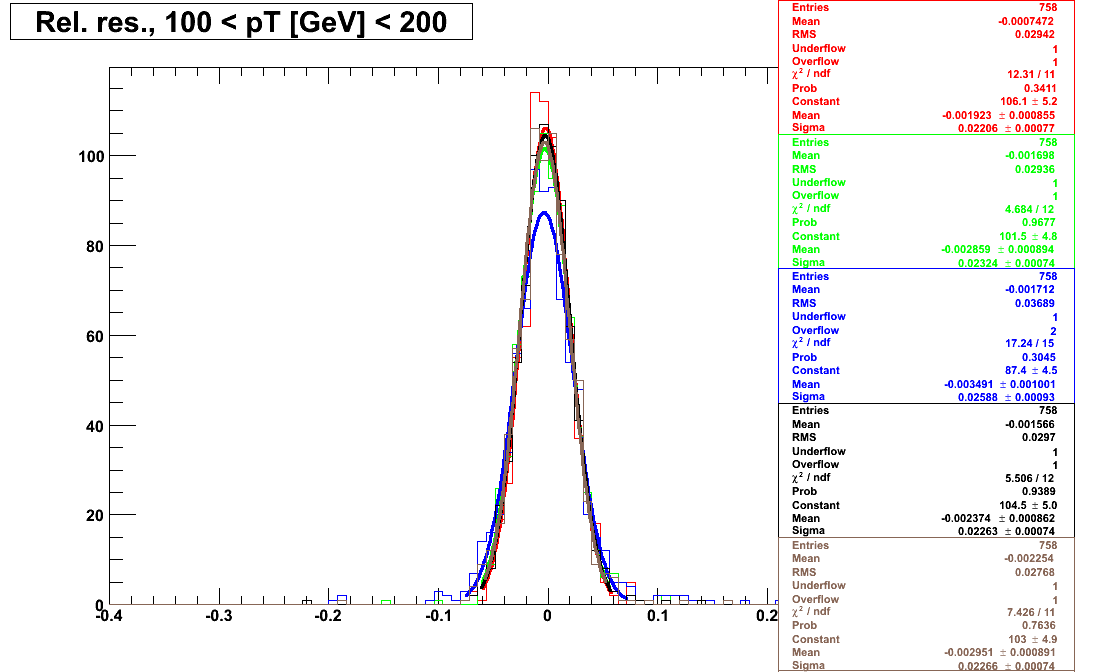
\includegraphics[width=\linewidth]{R1n-pT100200_7.png}}  % V11
\only<3>{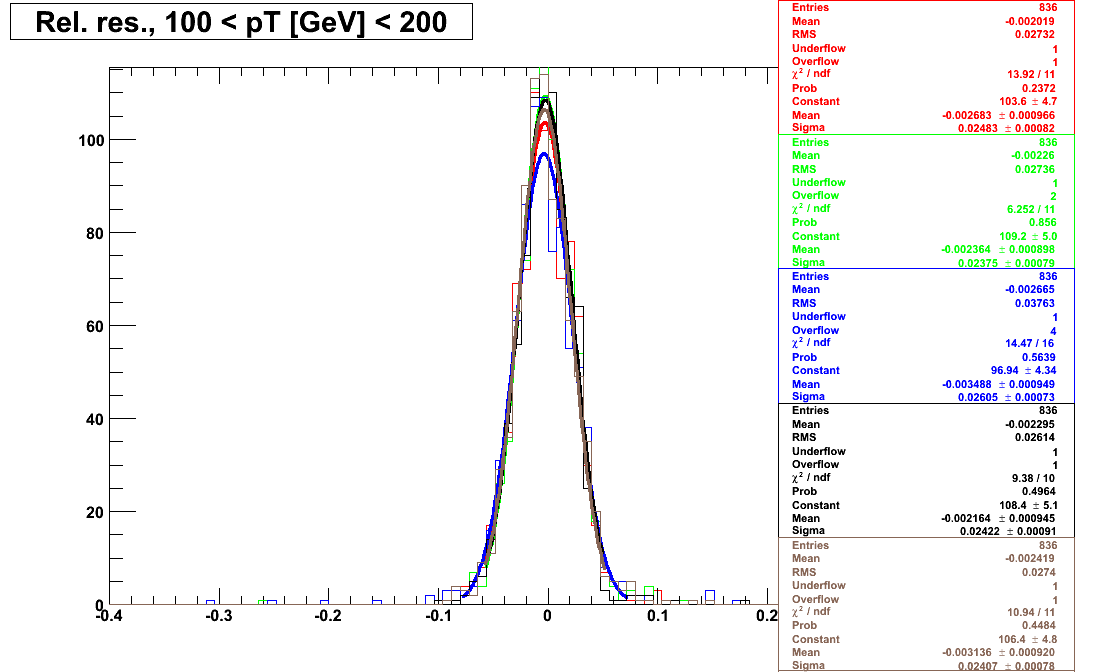
\includegraphics[width=\linewidth]{R1n-pT100200_1.png}}  % without latest tracker (May 25)
\only<4>{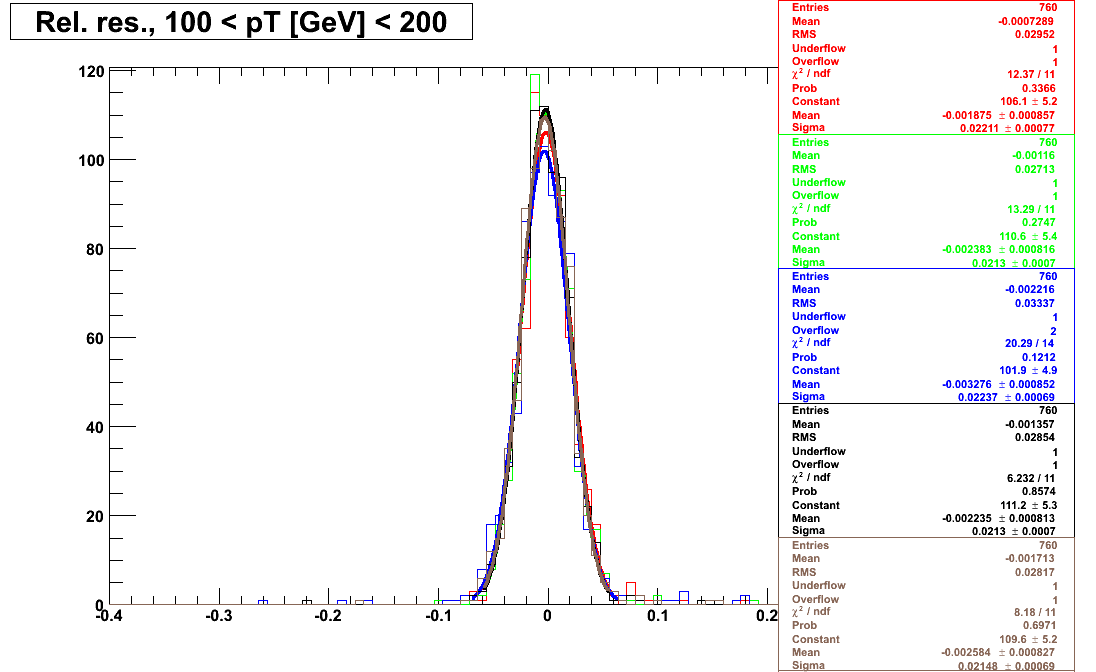
\includegraphics[width=\linewidth]{R1n-pT100200_4.png}}  % with latest tracker (May 29)
\column{0.2\linewidth}
\mbox{ }

\vspace{4 cm}
\textcolor{darkblue}{\scriptsize J.~Tucker}
\end{columns}
\end{frame}

\begin{frame}
\frametitle{Summary of barrel validation}
\begin{itemize}\setlength{\itemsep}{0.25 cm}
\item We know that consistency with updated tracker alignment means
  changing muon chamber positions (not angles) by $\sigma \sim 2$~mm
\item Something happened to the segment extrapolation test: it's not
  representing the changes we put in (angles change dramatically)
\begin{itemize}
\item can't use it to test May 29 alignment
\end{itemize}
\item Cosmic charge splitting indicates improvement with May 29
  alignment (based on latest tracker)
\end{itemize}

\vfill
\hspace{-0.83 cm} \textcolor{darkblue}{\Large An aside, for context}
\begin{itemize}\setlength{\itemsep}{0.35 cm}
\item 2008 MC $\frac{\left(1/p_T\right)_{\mbox{\tiny meas}} - \left(1/p_T\right)_{\mbox{\tiny gen}}}{\sqrt{2} \, \left(1/p_T\right)_{\mbox{\tiny gen}}}$ \textcolor{darkgreen}{first-muon station (FMS)} resolution:

\vspace{0.1 cm}
IDEAL: 2\%, CSA08 10~pb$^{-1}$: 3\%, STARTUP: 6\% at 200~GeV
\item Cosmic splitting \textcolor{darkgreen}{FMS}: May 25: 5.2\% May 29: 4.5\% at 200~GeV
\end{itemize}
\end{frame}

\begin{frame}
\frametitle{Endcap constants}
\begin{itemize}
\item Photogrammetry $+$ hardware disk-bending $+$ disk positions \mbox{from tracks\hspace{-1 cm}}
\item New fits to whole-ring local residuals (next few pages)
\item 3-DOF global corrections to 4 disks:

\vspace{-0.5 cm}
\begin{columns}
\column{0.7\linewidth}
\renewcommand{\arraystretch}{1.25}
\begin{tabular}{c c c c}
& $\delta_{\phi}$ (mrad) & $\delta_x$ (mm) & $\delta_y$ (mm) \\
ME$+$1 & 0.06 & 3.3 & $-$0.1 \\
ME$+$2,3 & $-$0.04 & 1.7 & 2.6 \\
ME$-$1 & 1.0 & 3.2 &$-$3.7 \\
ME$-$2,3 & 1.44 & 4.4 & $-$0.1
\end{tabular}
\column{0.35\linewidth}
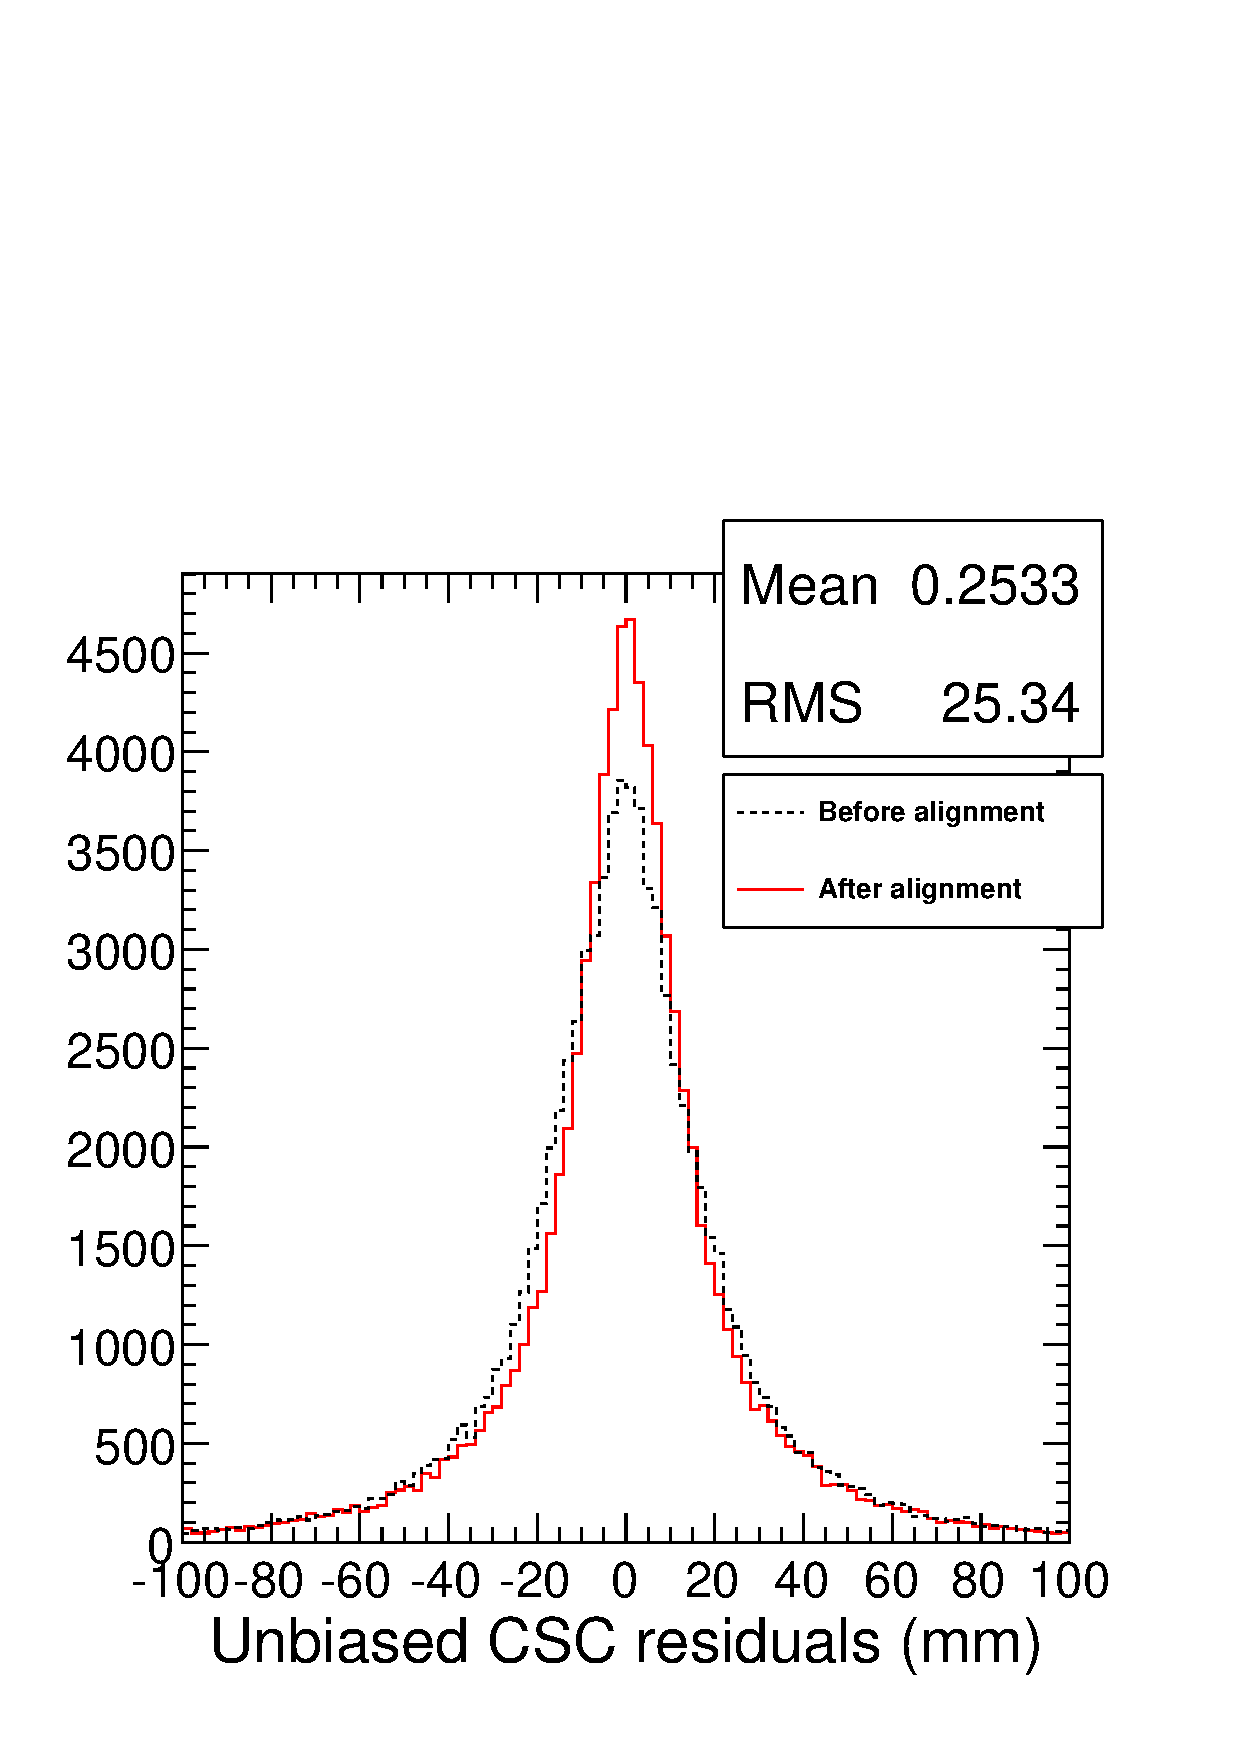
\includegraphics[width=\linewidth]{endcap_residuals.pdf}
\end{columns}

\item ``Non-definitive'' transfer line numbers from Jim B.

\begin{center}\renewcommand{\arraystretch}{1.25}
\begin{tabular}{c c c c}
& $\delta_{\phi}$ (mrad) & $\delta_x$ (mm) & $\delta_y$ (mm) \\
ME$+$2,3 minus ME$+$1 & 0.98 & 1.03 & $-$1.28 \\
ME$-$2,3 minus ME$-$1 & 0.65 & 3.7 & 4.32
\end{tabular}
\end{center}

\item Same rough scale; no wild disagreements
\end{itemize}
\end{frame}

\begin{frame}
\frametitle{Alignment fits (\only<1>{1}\only<2>{2}\only<3>{3}\only<4>{4}/4)}

\begin{columns}
\column{0.7\linewidth}
\only<1>{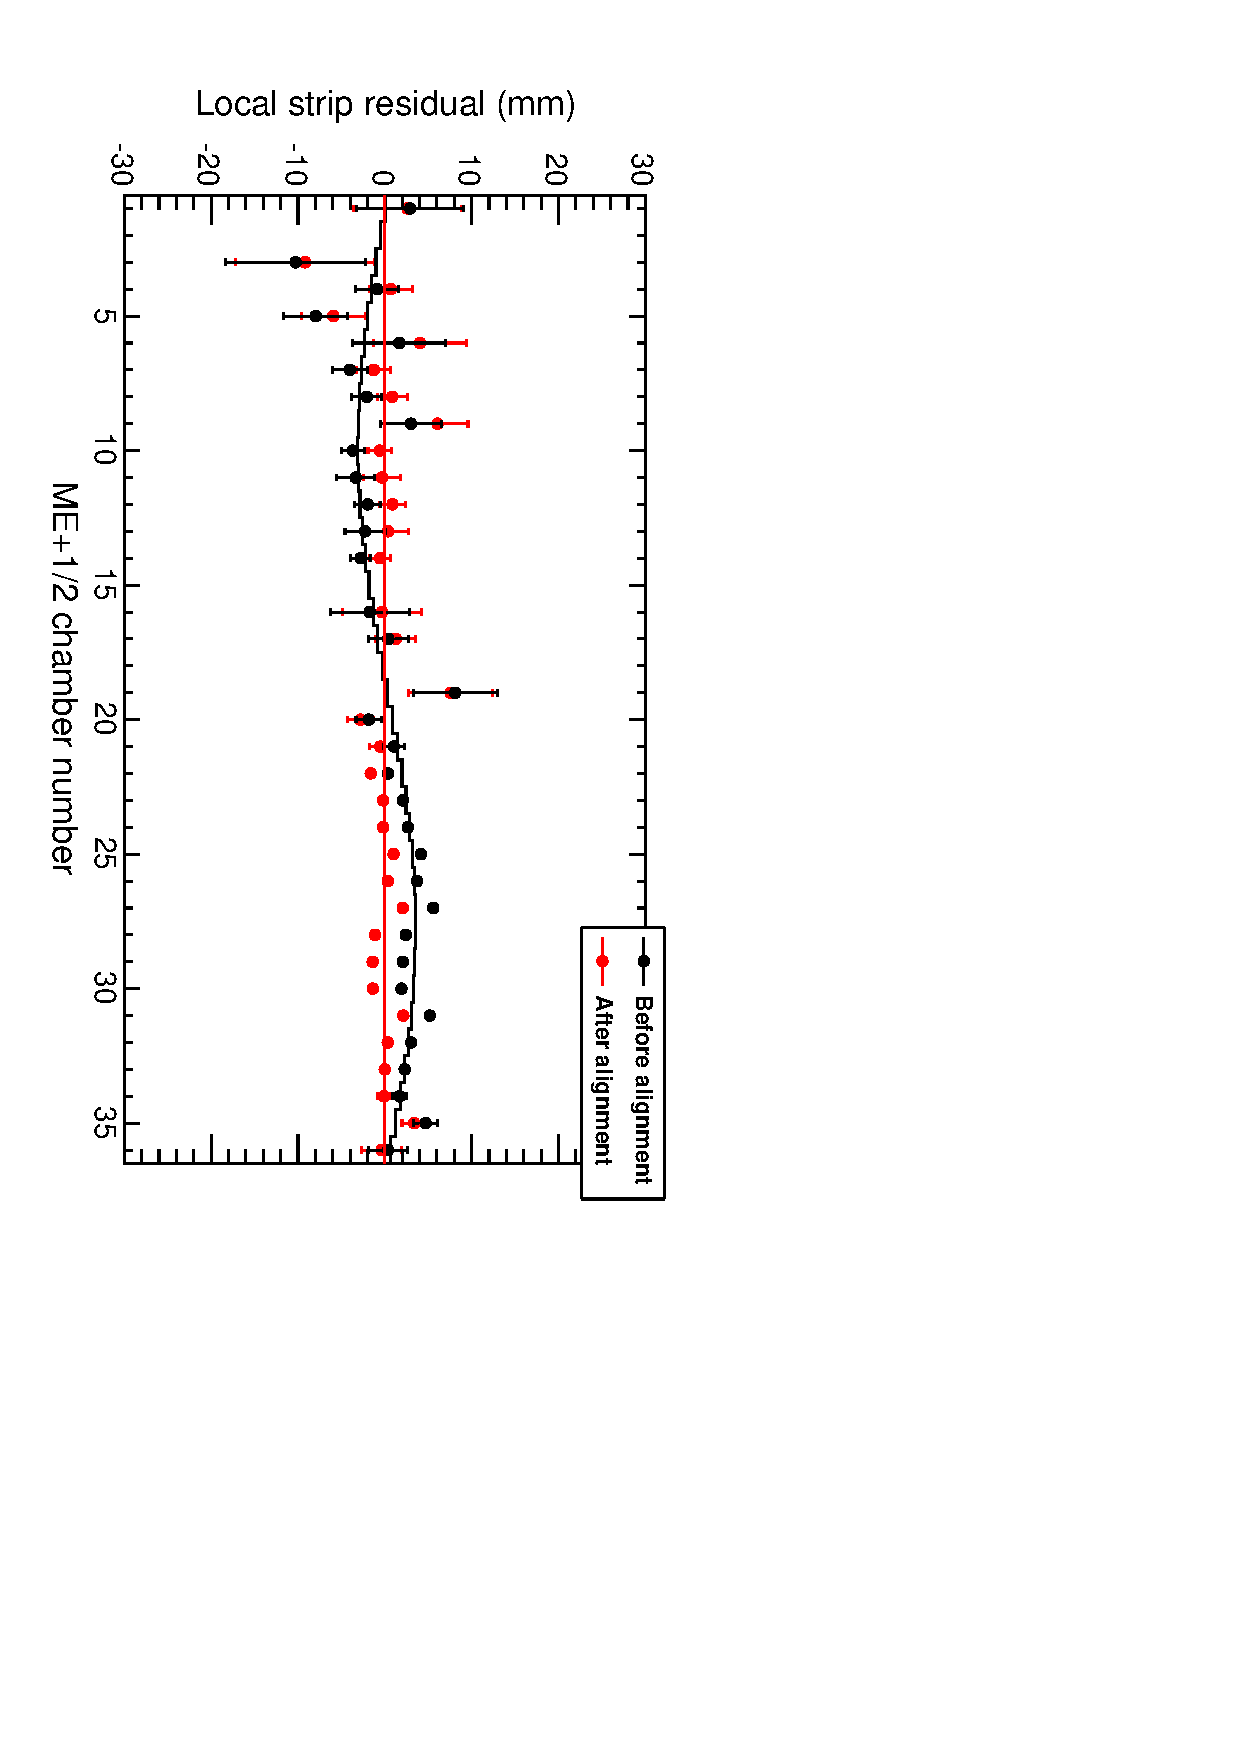
\includegraphics[height=\linewidth, angle=90]{endcap_mep12.pdf}}
\only<2>{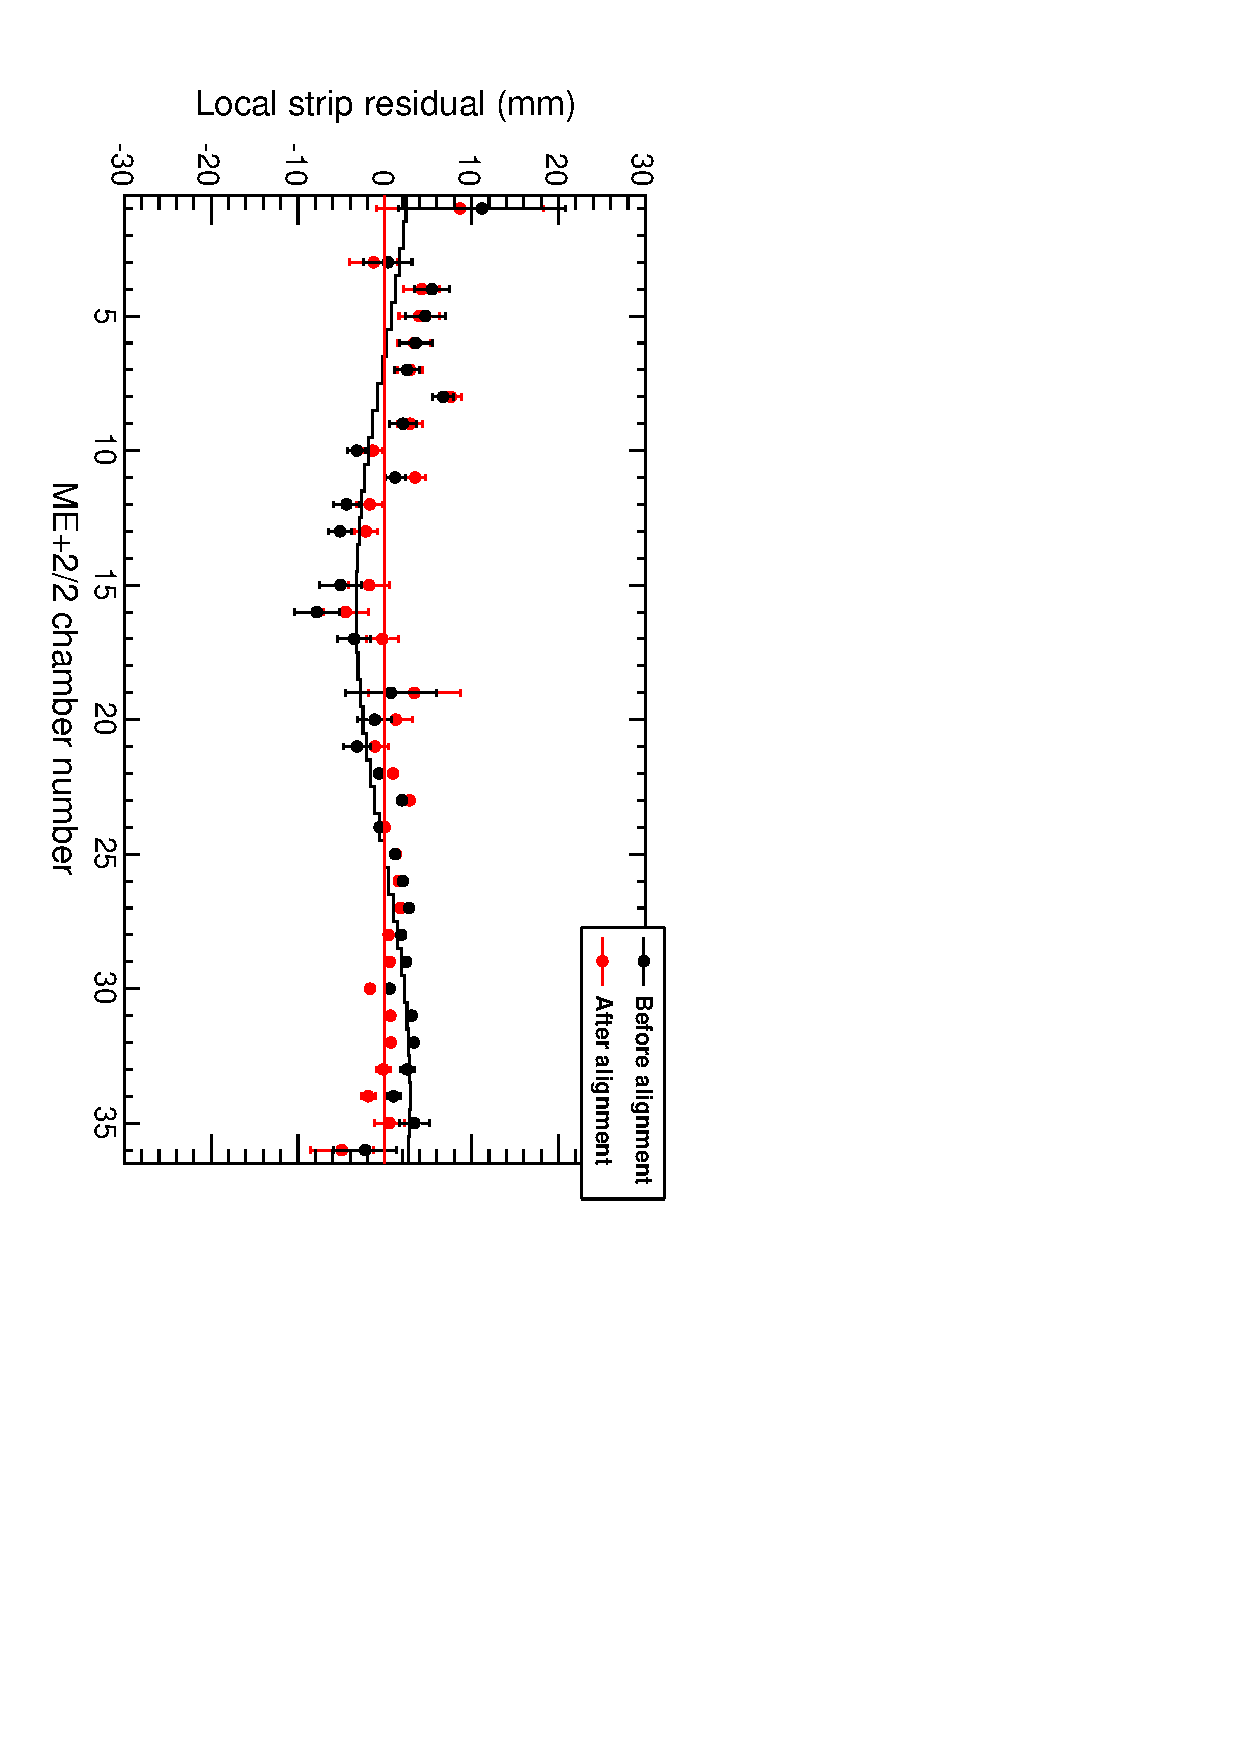
\includegraphics[height=\linewidth, angle=90]{endcap_mep22.pdf}}
\only<3>{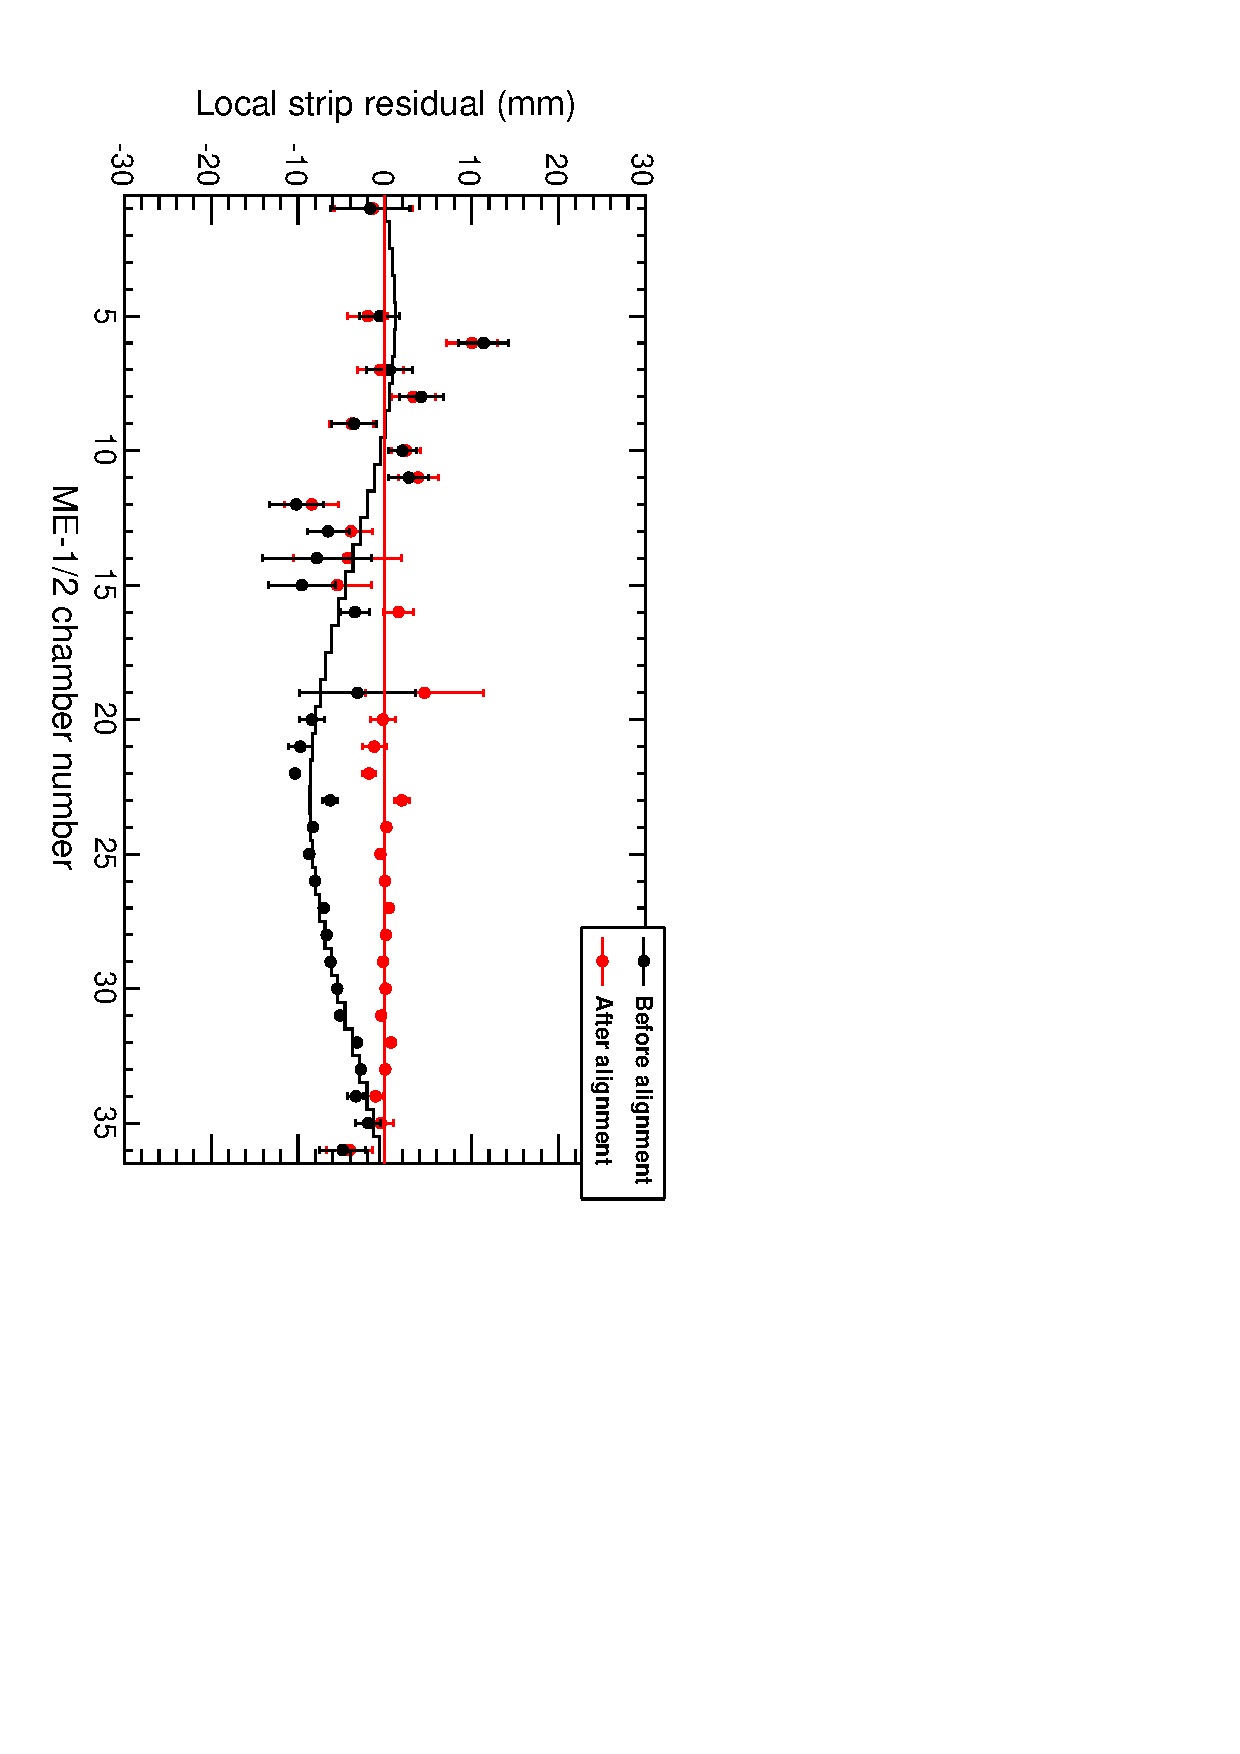
\includegraphics[height=\linewidth, angle=90]{endcap_mem12.pdf}}
\only<4>{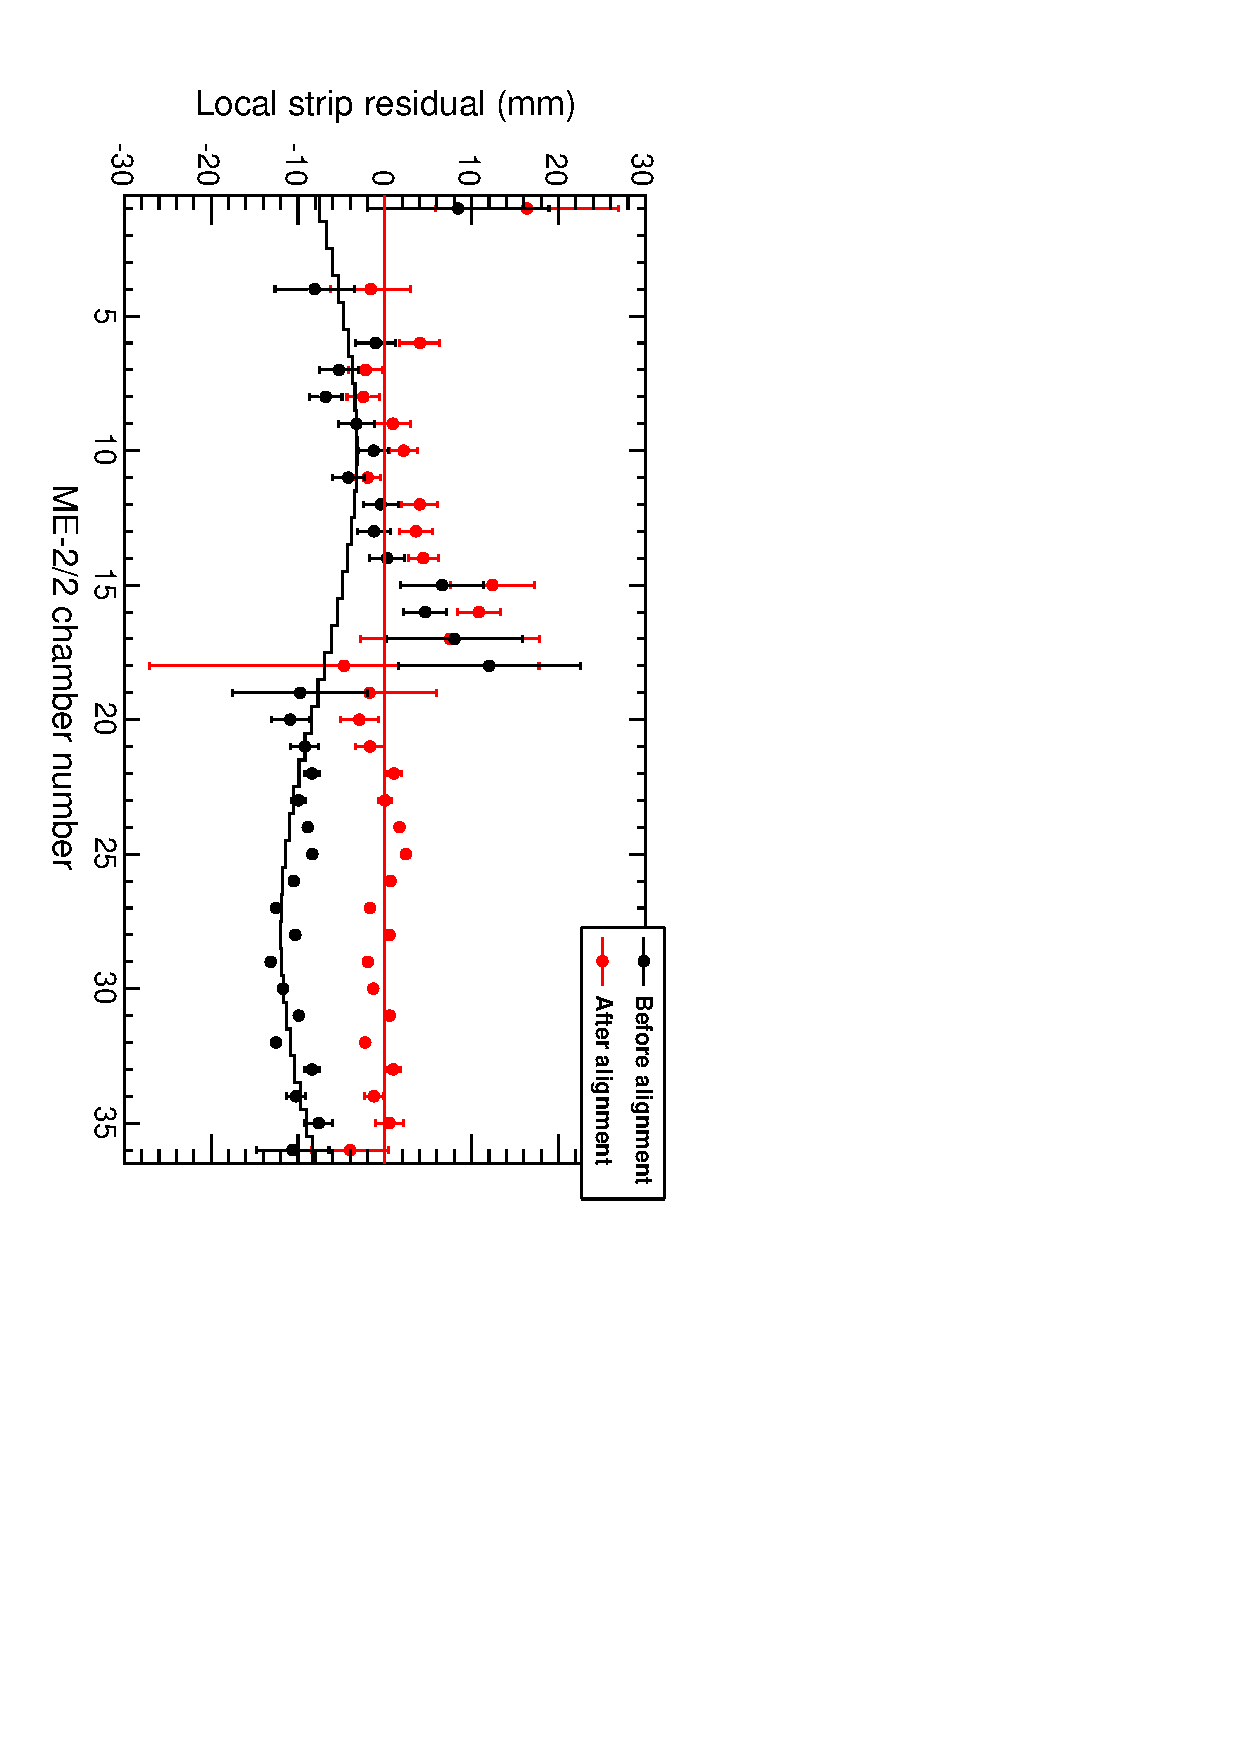
\includegraphics[height=\linewidth, angle=90]{endcap_mem22.pdf}}

\only<1>{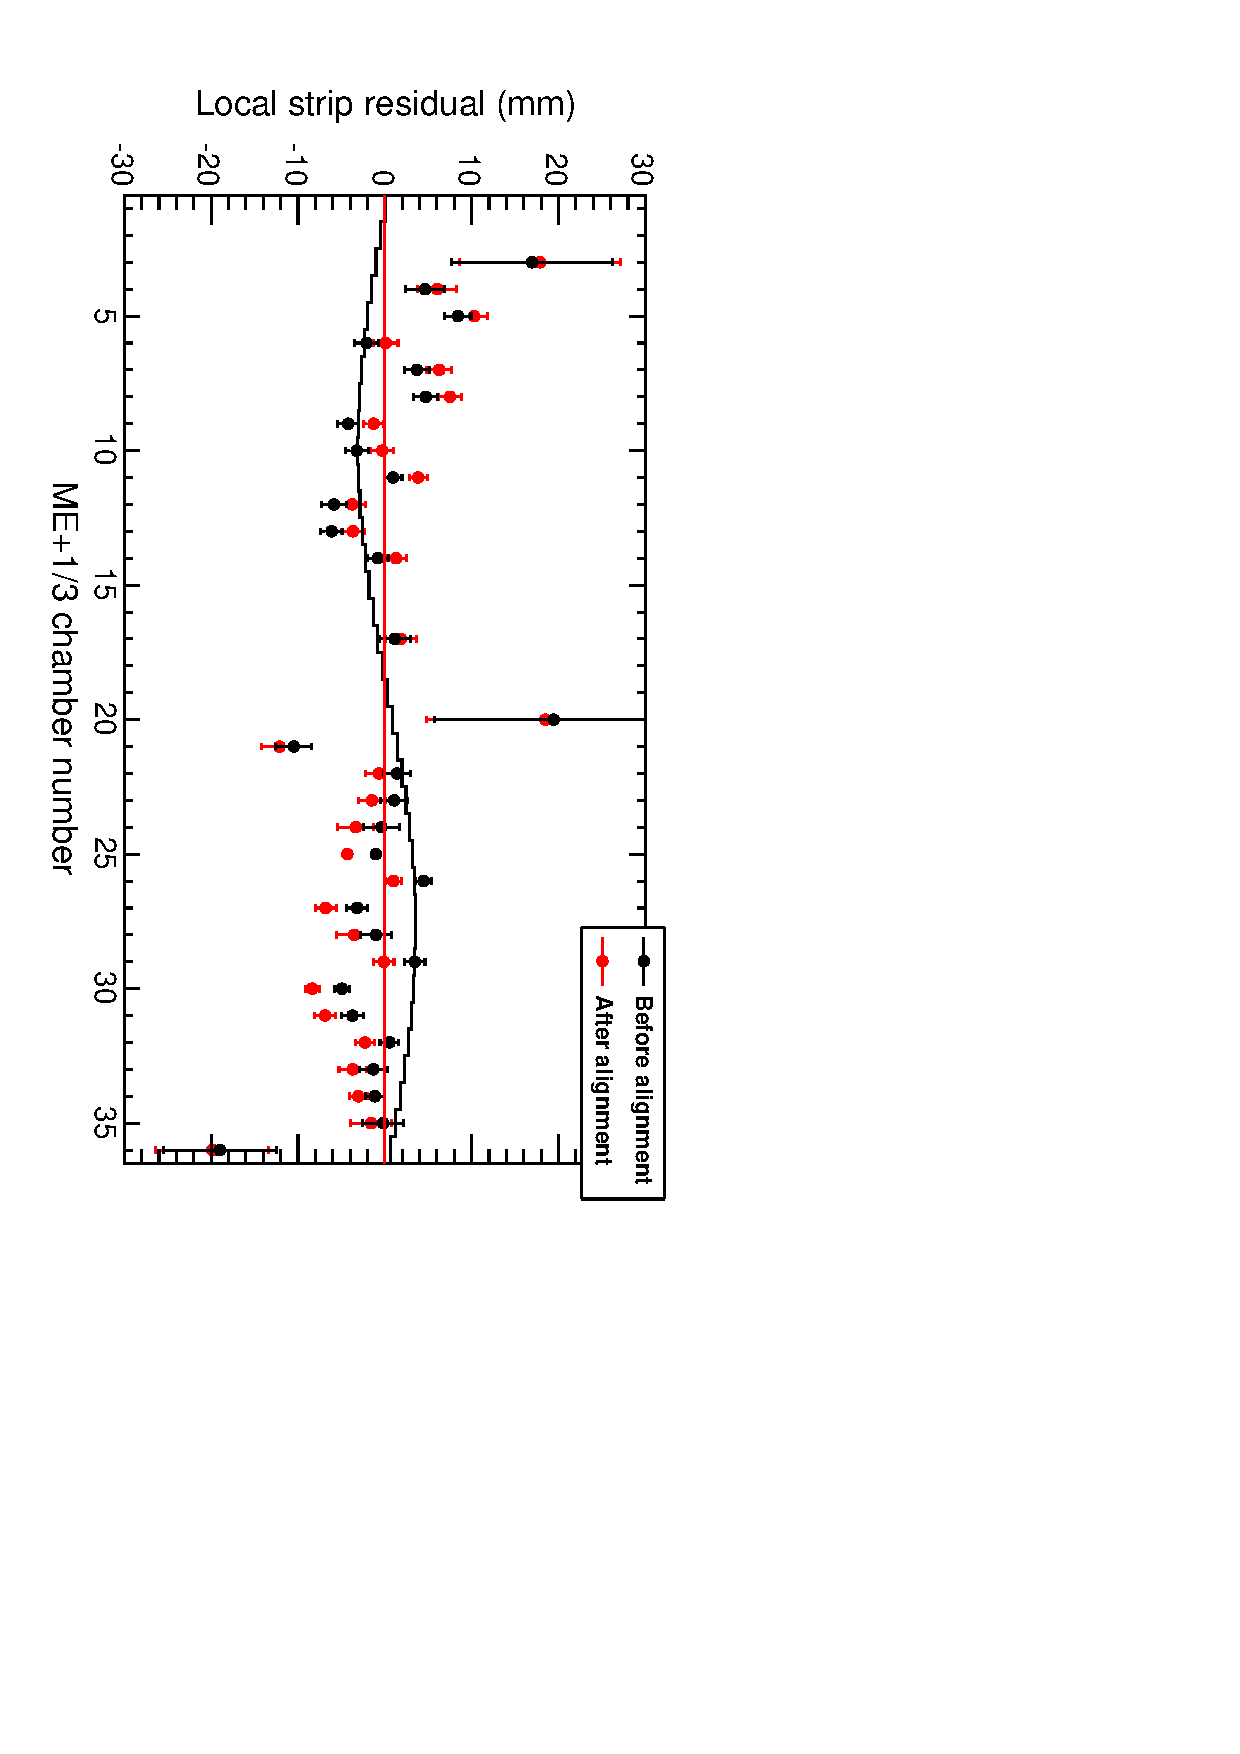
\includegraphics[height=\linewidth, angle=90]{endcap_mep13.pdf}}
\only<2>{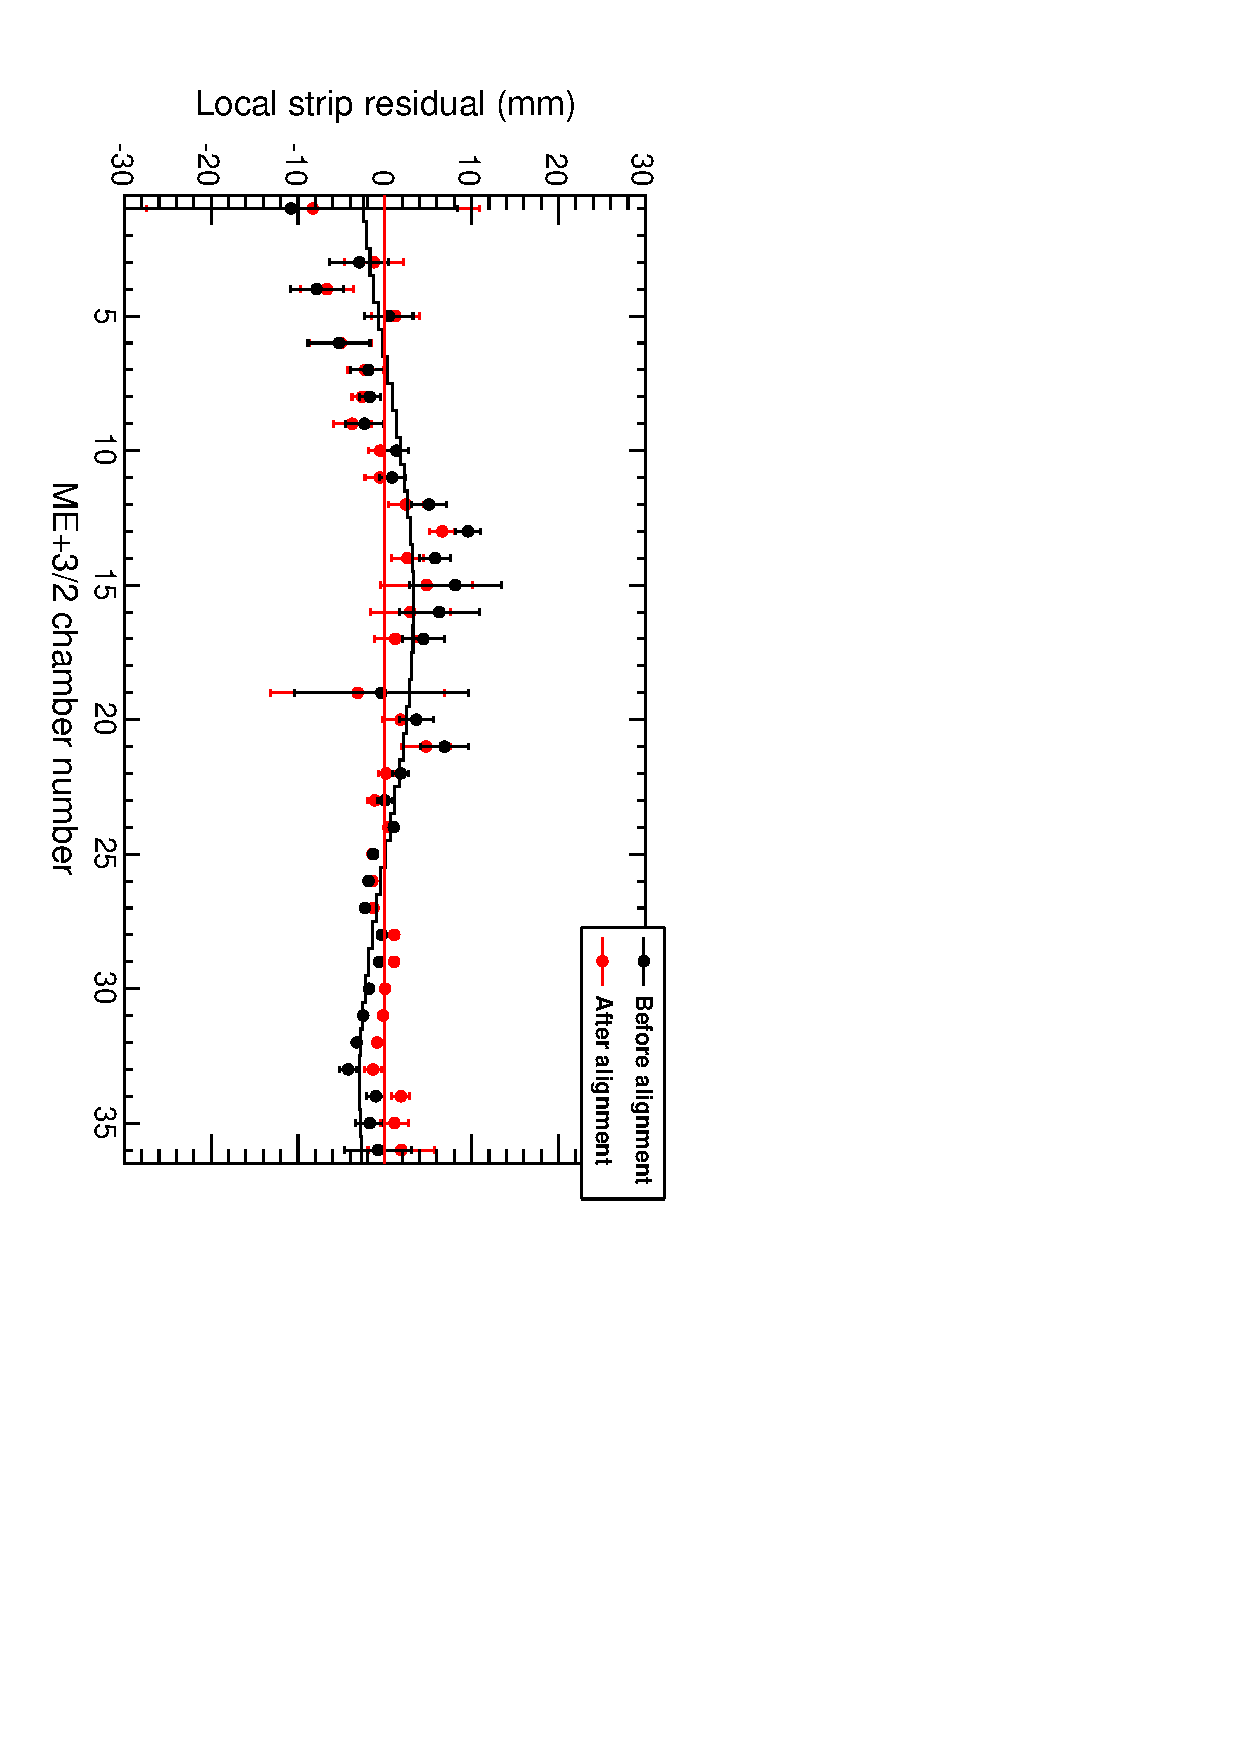
\includegraphics[height=\linewidth, angle=90]{endcap_mep32.pdf}}
\only<3>{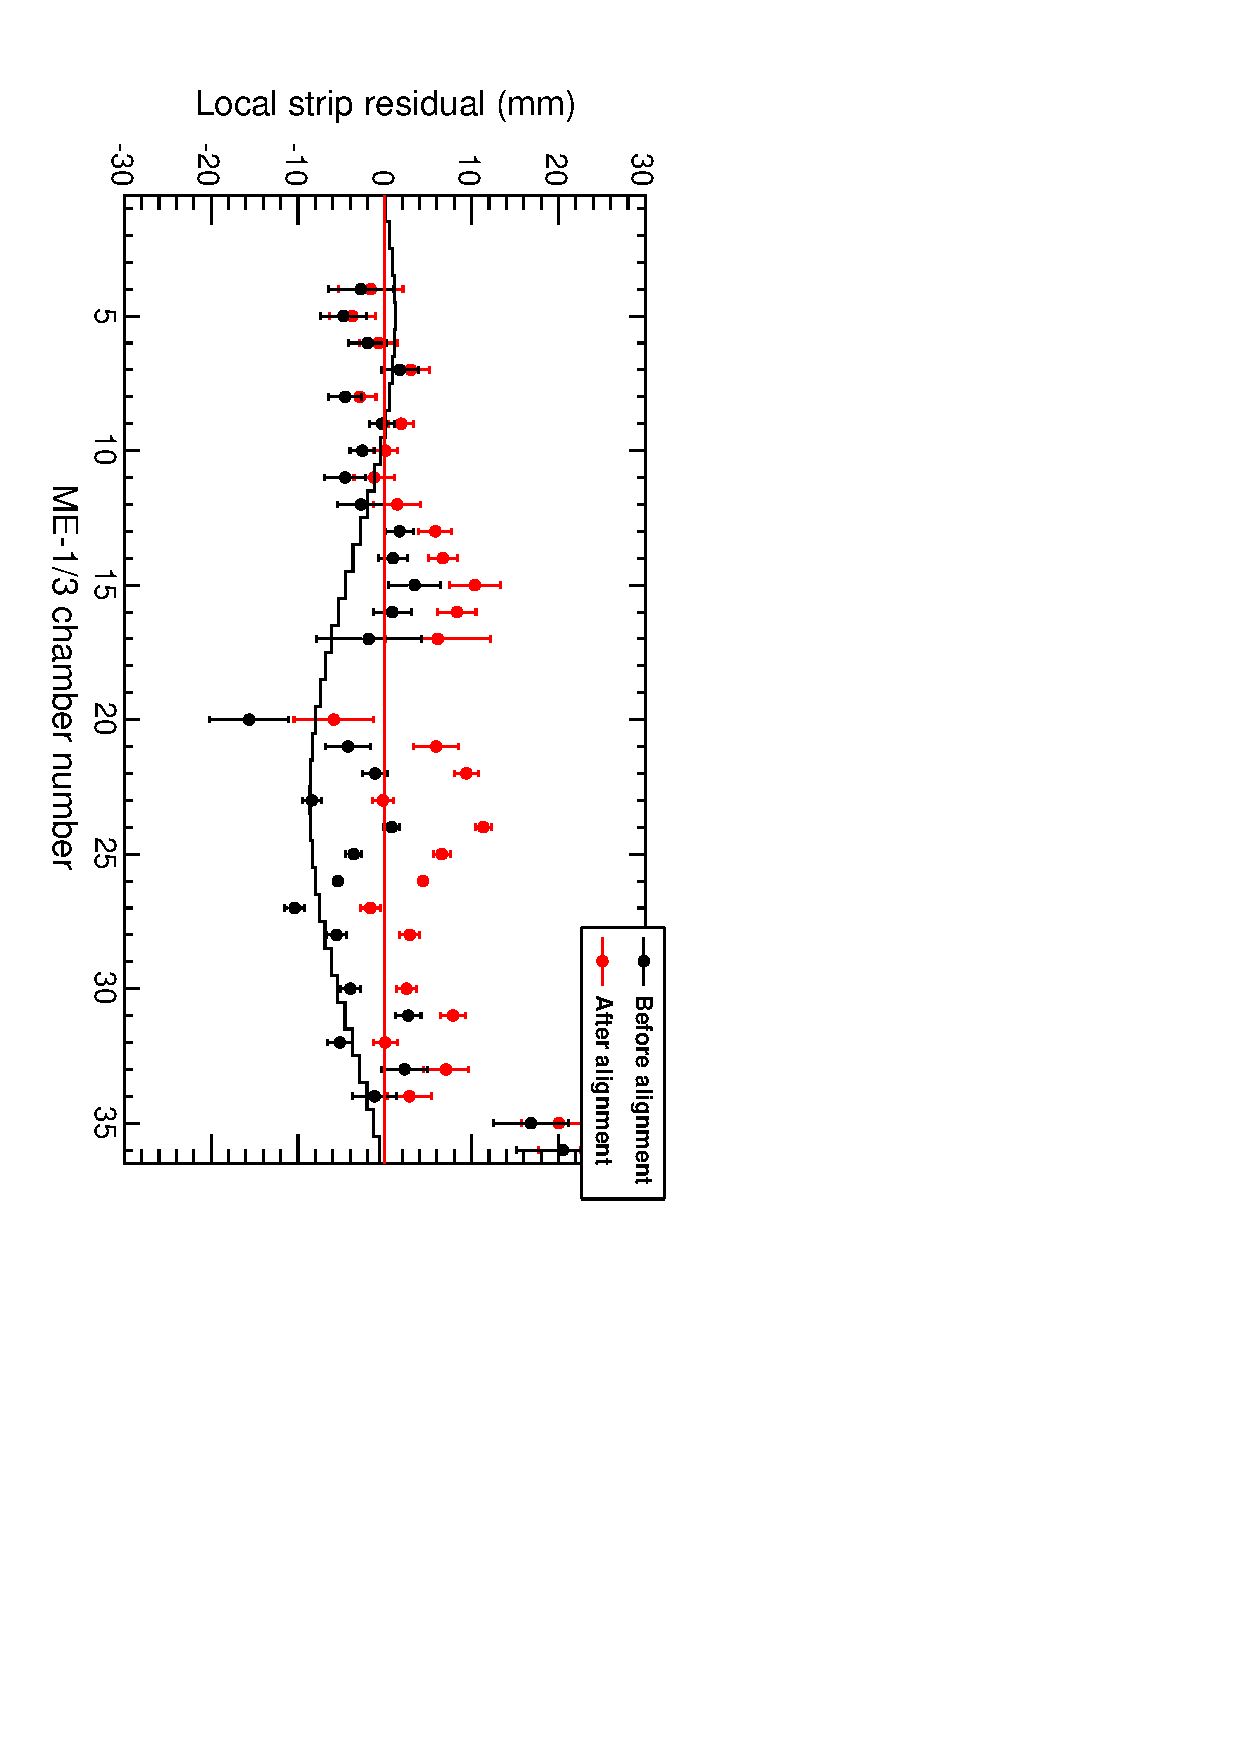
\includegraphics[height=\linewidth, angle=90]{endcap_mem13.pdf}}
\only<4>{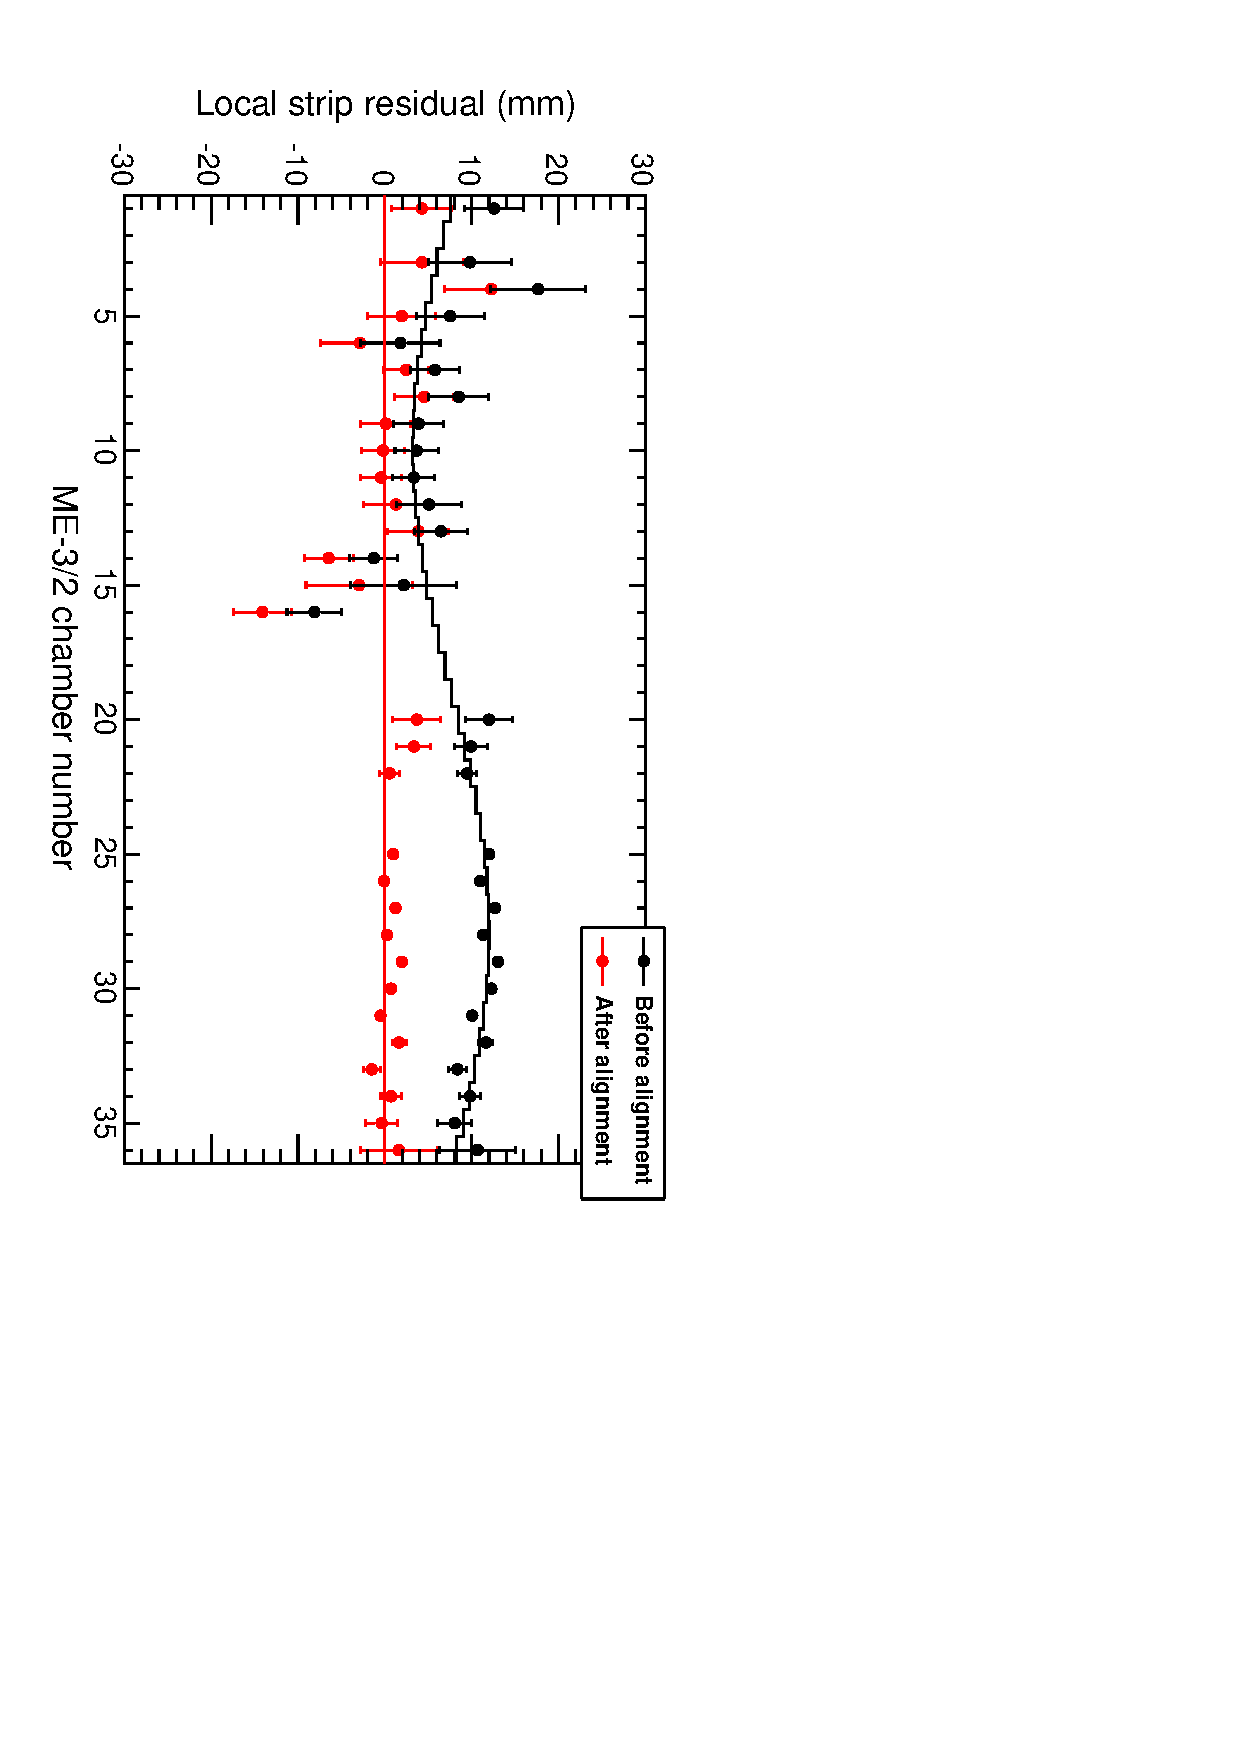
\includegraphics[height=\linewidth, angle=90]{endcap_mem32.pdf}}

\column{0.3\linewidth}
\only<1>{ME$+$1/2 (fitted)}
\only<2>{ME$+$2/2 (fitted)}
\only<3>{ME$-$1/2 (fitted)}
\only<4>{ME$-$2/2 (fitted)}

\vspace{3 cm}
\only<1>{ME$+$1/3 (overlay \\ \hfill ME$+$1/2 fit)}
\only<2>{ME$+$3/2 (overlay \\ \hfill ME$+$2/2 fit)}
\only<3>{ME$-$1/3 (overlay \\ \hfill ME$-$1/2 fit)}
\only<4>{ME$-$3/2 (overlay \\ \hfill ME$-$2/2 fit)}
\end{columns}
\end{frame}

\begin{frame}
\frametitle{Residuals differences}

\begin{columns}
\column{0.7\linewidth}
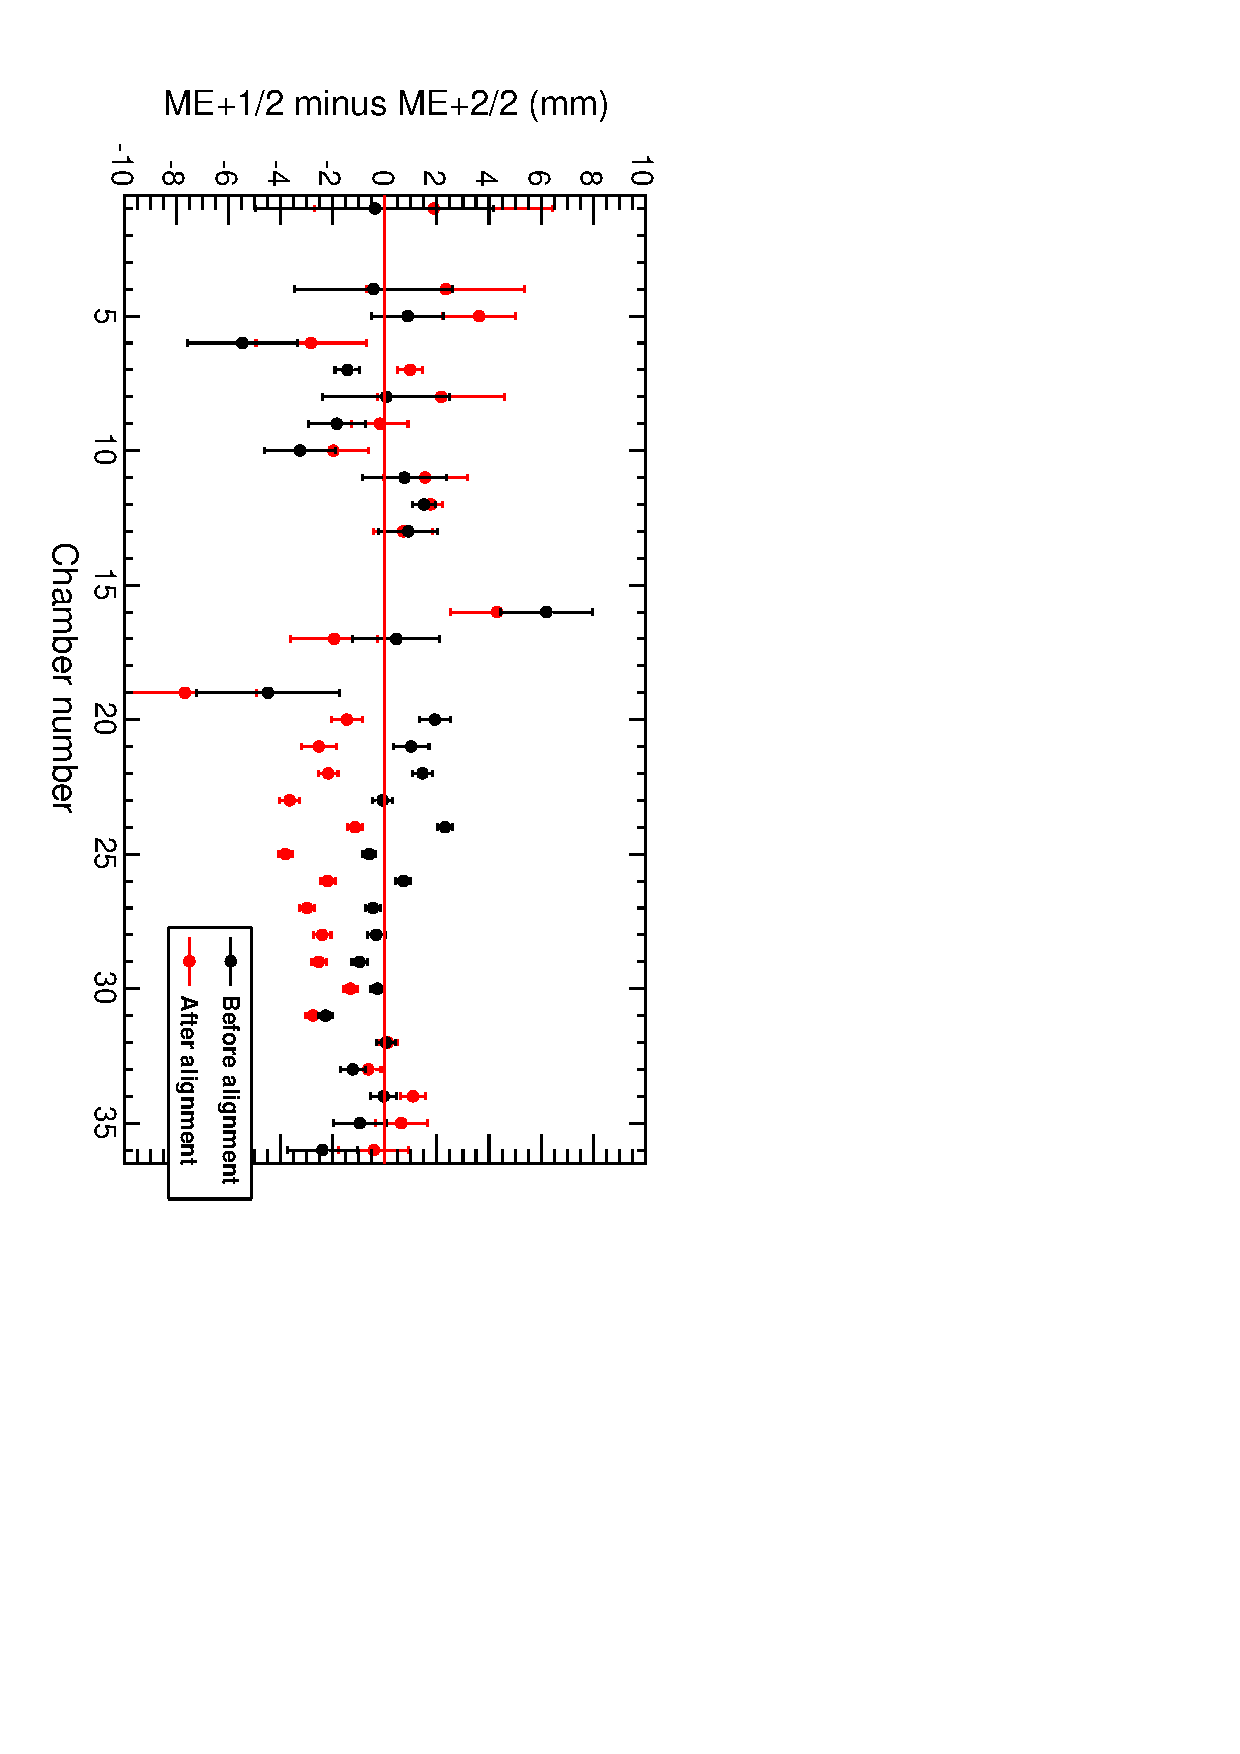
\includegraphics[height=\linewidth, angle=90]{endcap_diffplus.pdf}

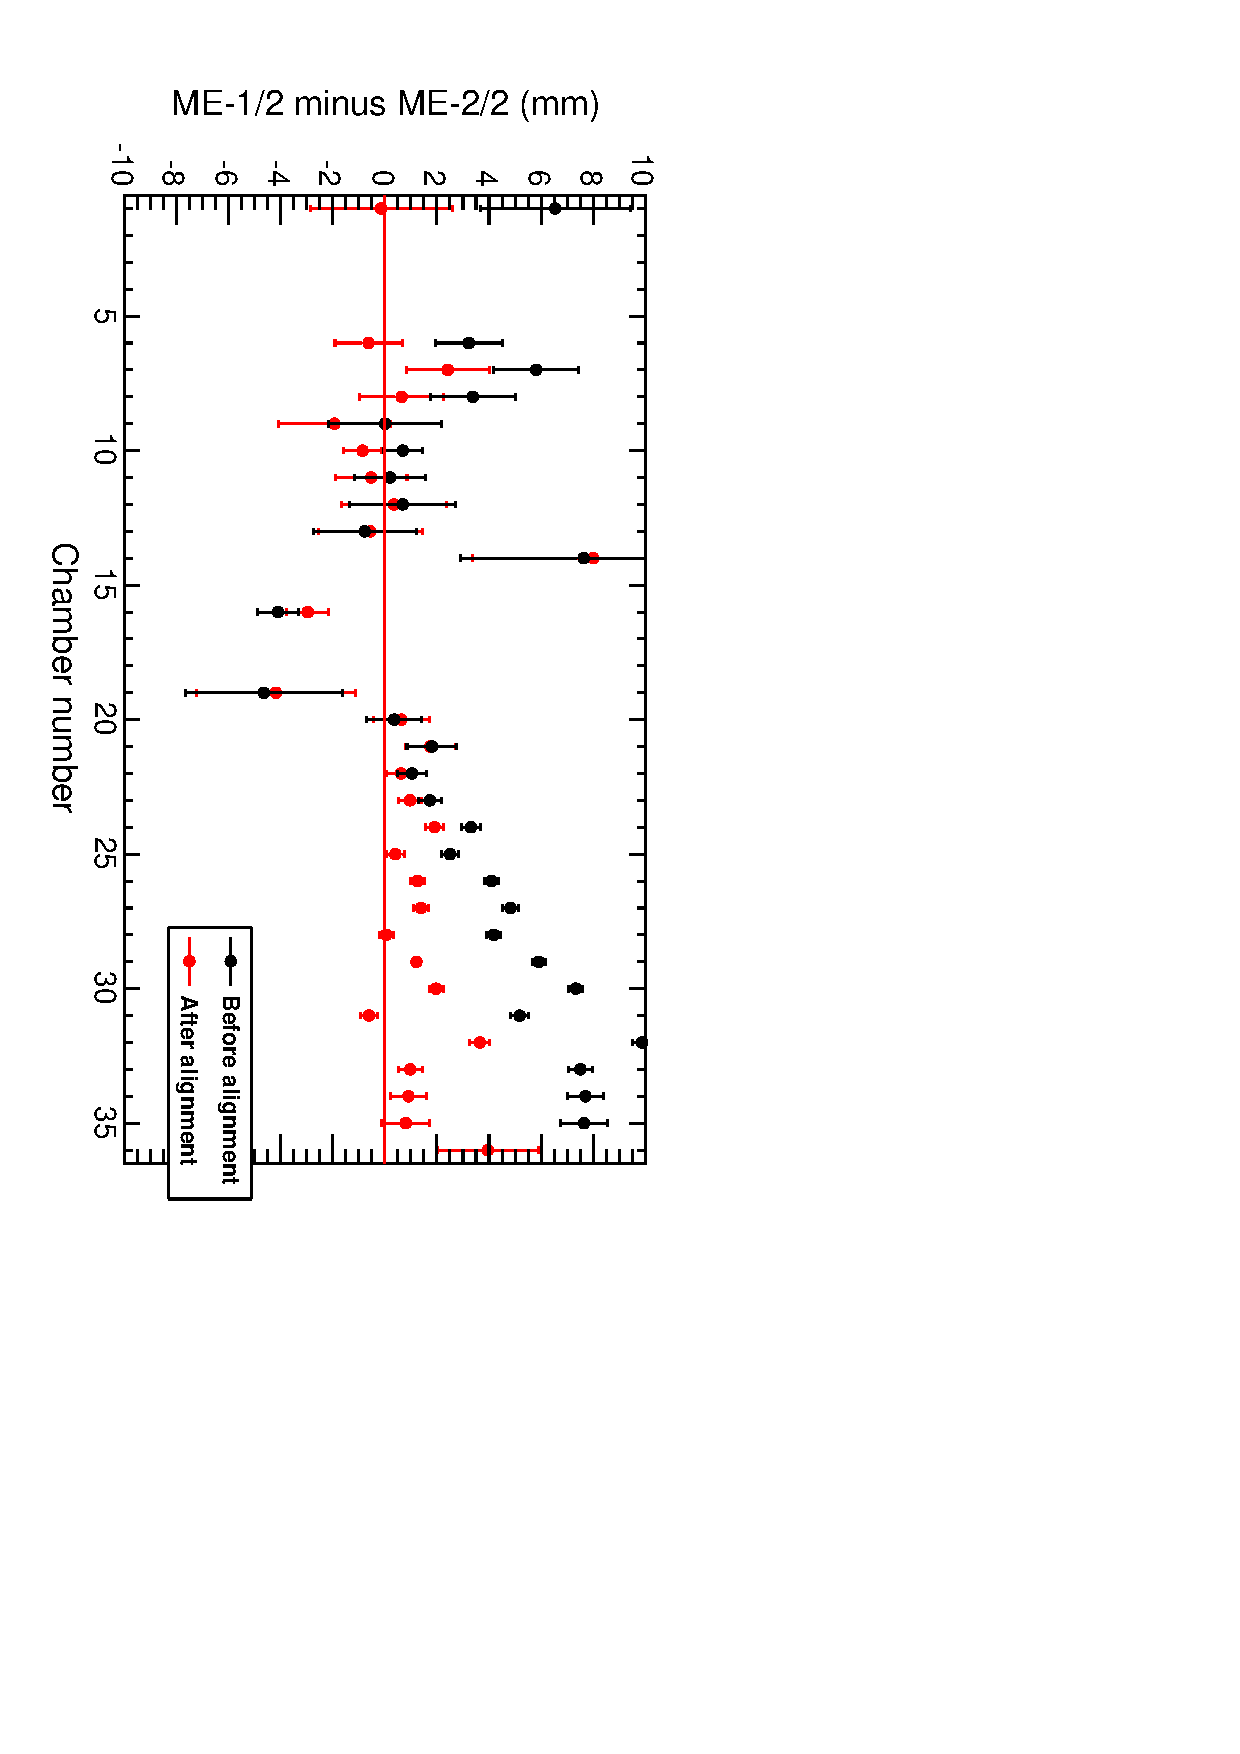
\includegraphics[height=\linewidth, angle=90]{endcap_diffminus.pdf}
\column{0.3\linewidth}
\scriptsize 
Residuals differences are equivalent to segment extrapolation with the CMSSW propagator and a momentum assumption (from tracker)

\vspace{0.3 cm}
More precise than absolute residuals and measure relative differences

\vspace{0.3 cm}
New information: an independent check on alignment
\end{columns}
\end{frame}

%% \section*{First section}
%% \begin{frame}
%% \begin{center}
%% \Huge \textcolor{blue}{First section}
%% \end{center}
%% \end{frame}

\begin{frame}
\frametitle{Backup: individual chambers}
\begin{itemize}
\item ME$-$2/2, before and \textcolor{red}{after} alignment (stats box applies to \textcolor{red}{after})
\item No weights, no fits, just a mean truncated at $\pm$100~mm
\end{itemize}

\vfill
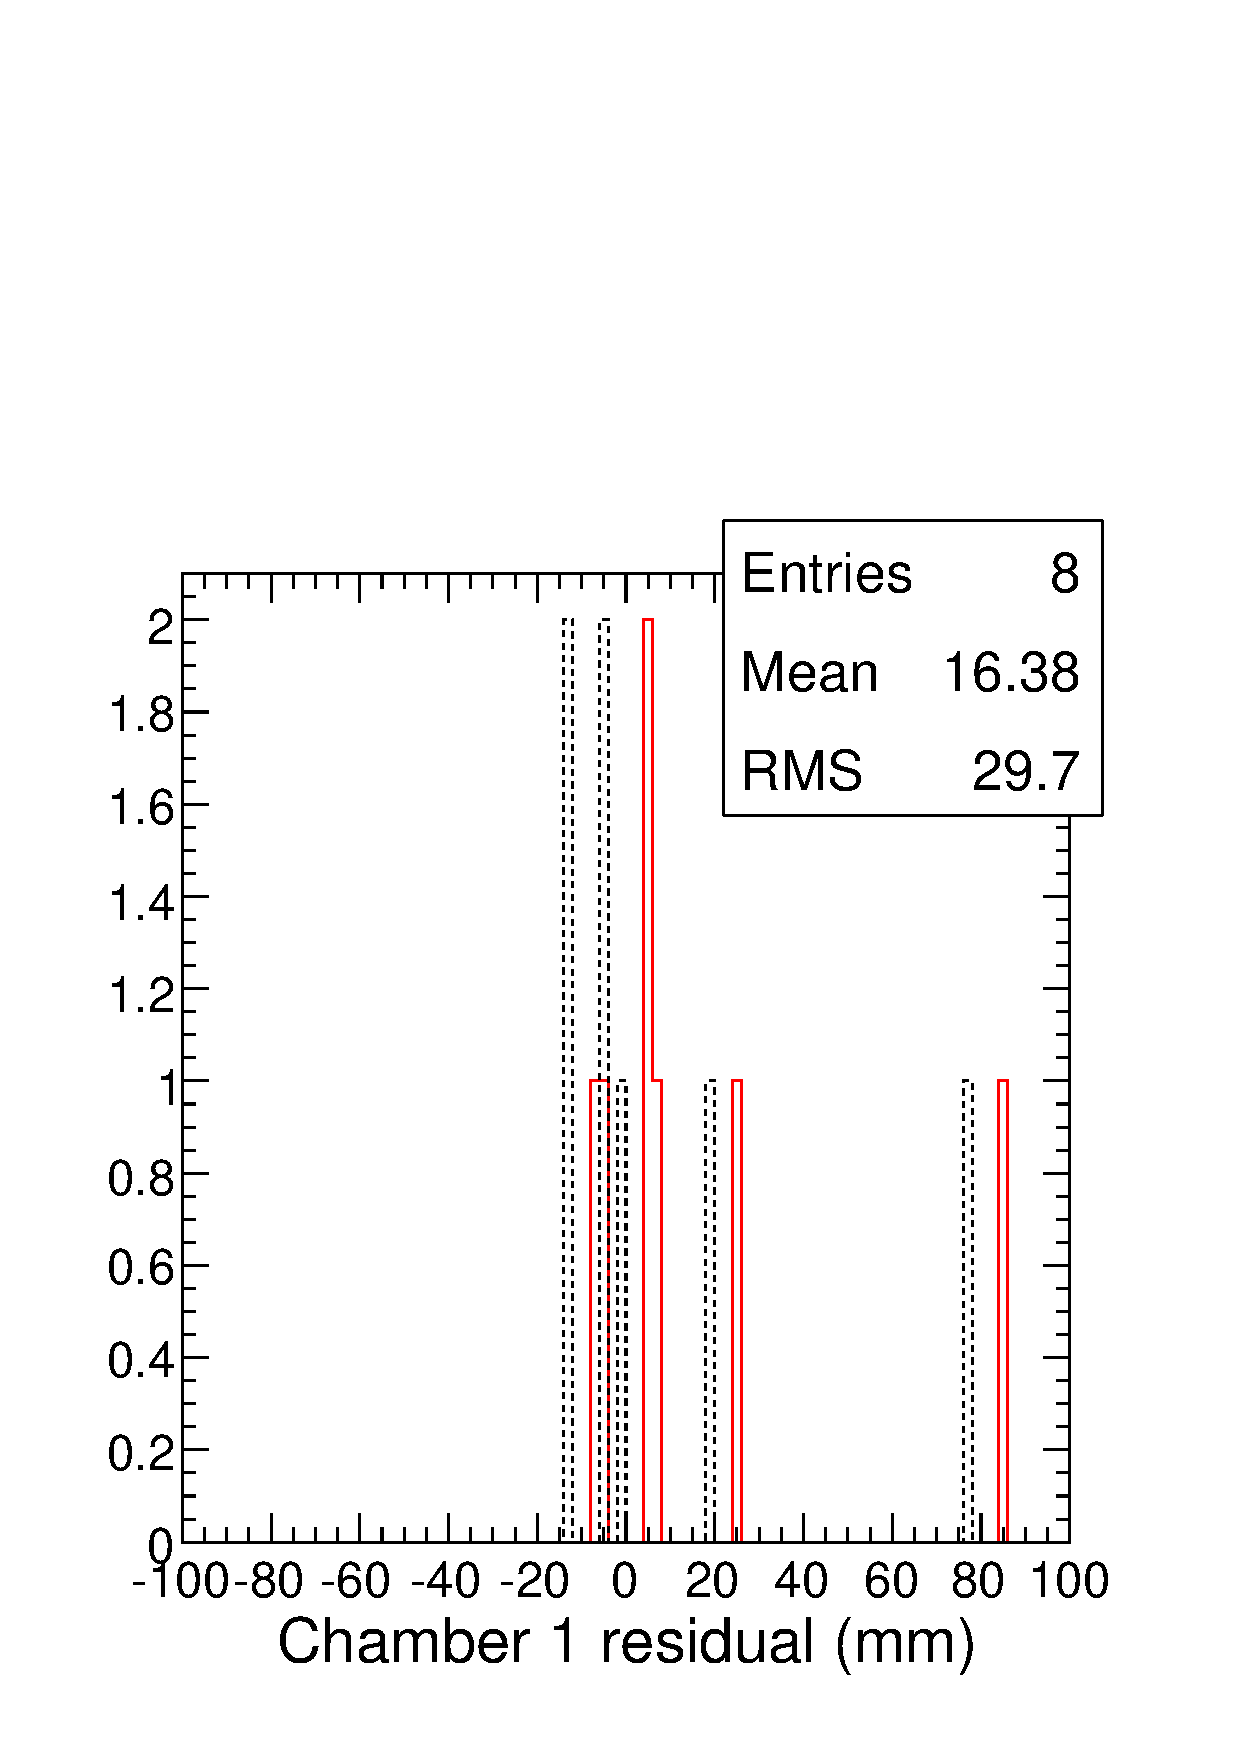
\includegraphics[width=0.11\linewidth]{endcap_mem22_1.pdf}
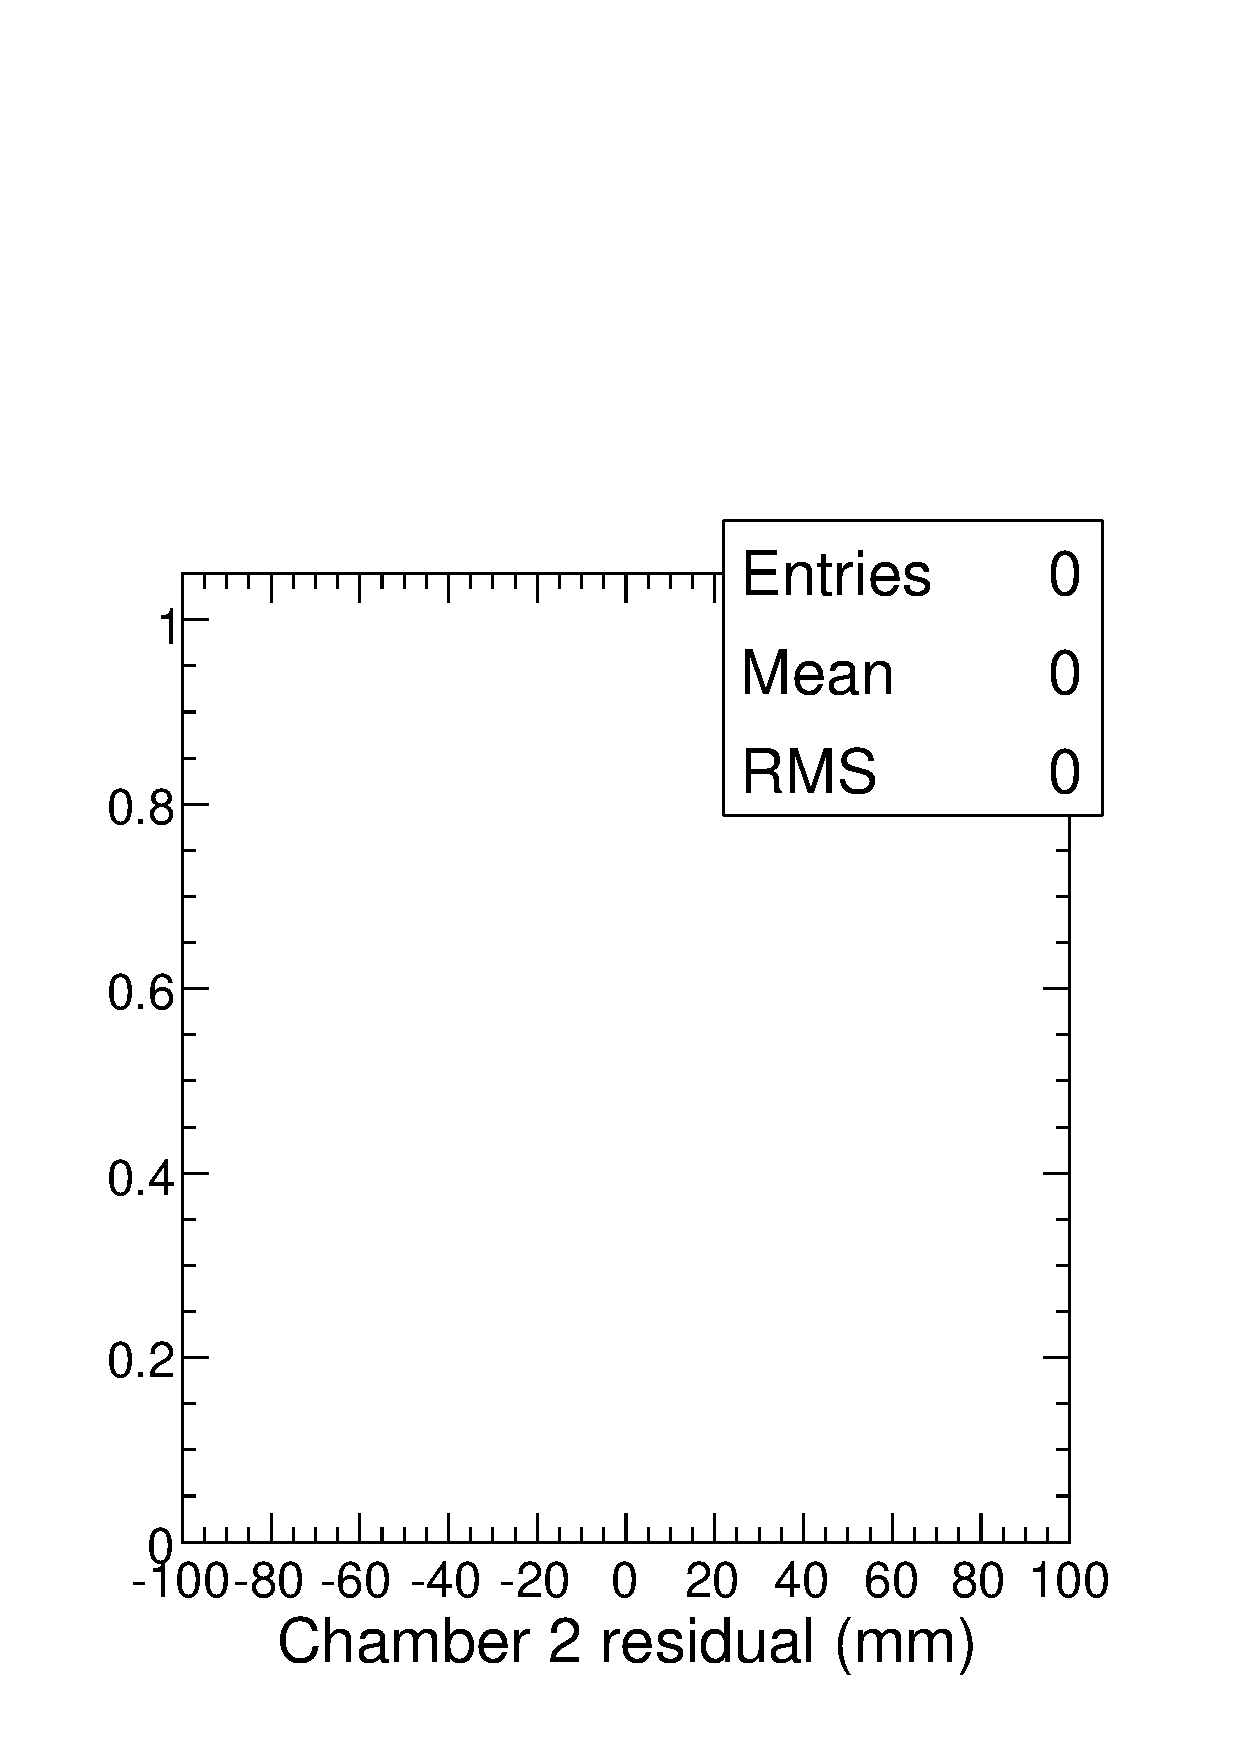
\includegraphics[width=0.11\linewidth]{endcap_mem22_2.pdf}
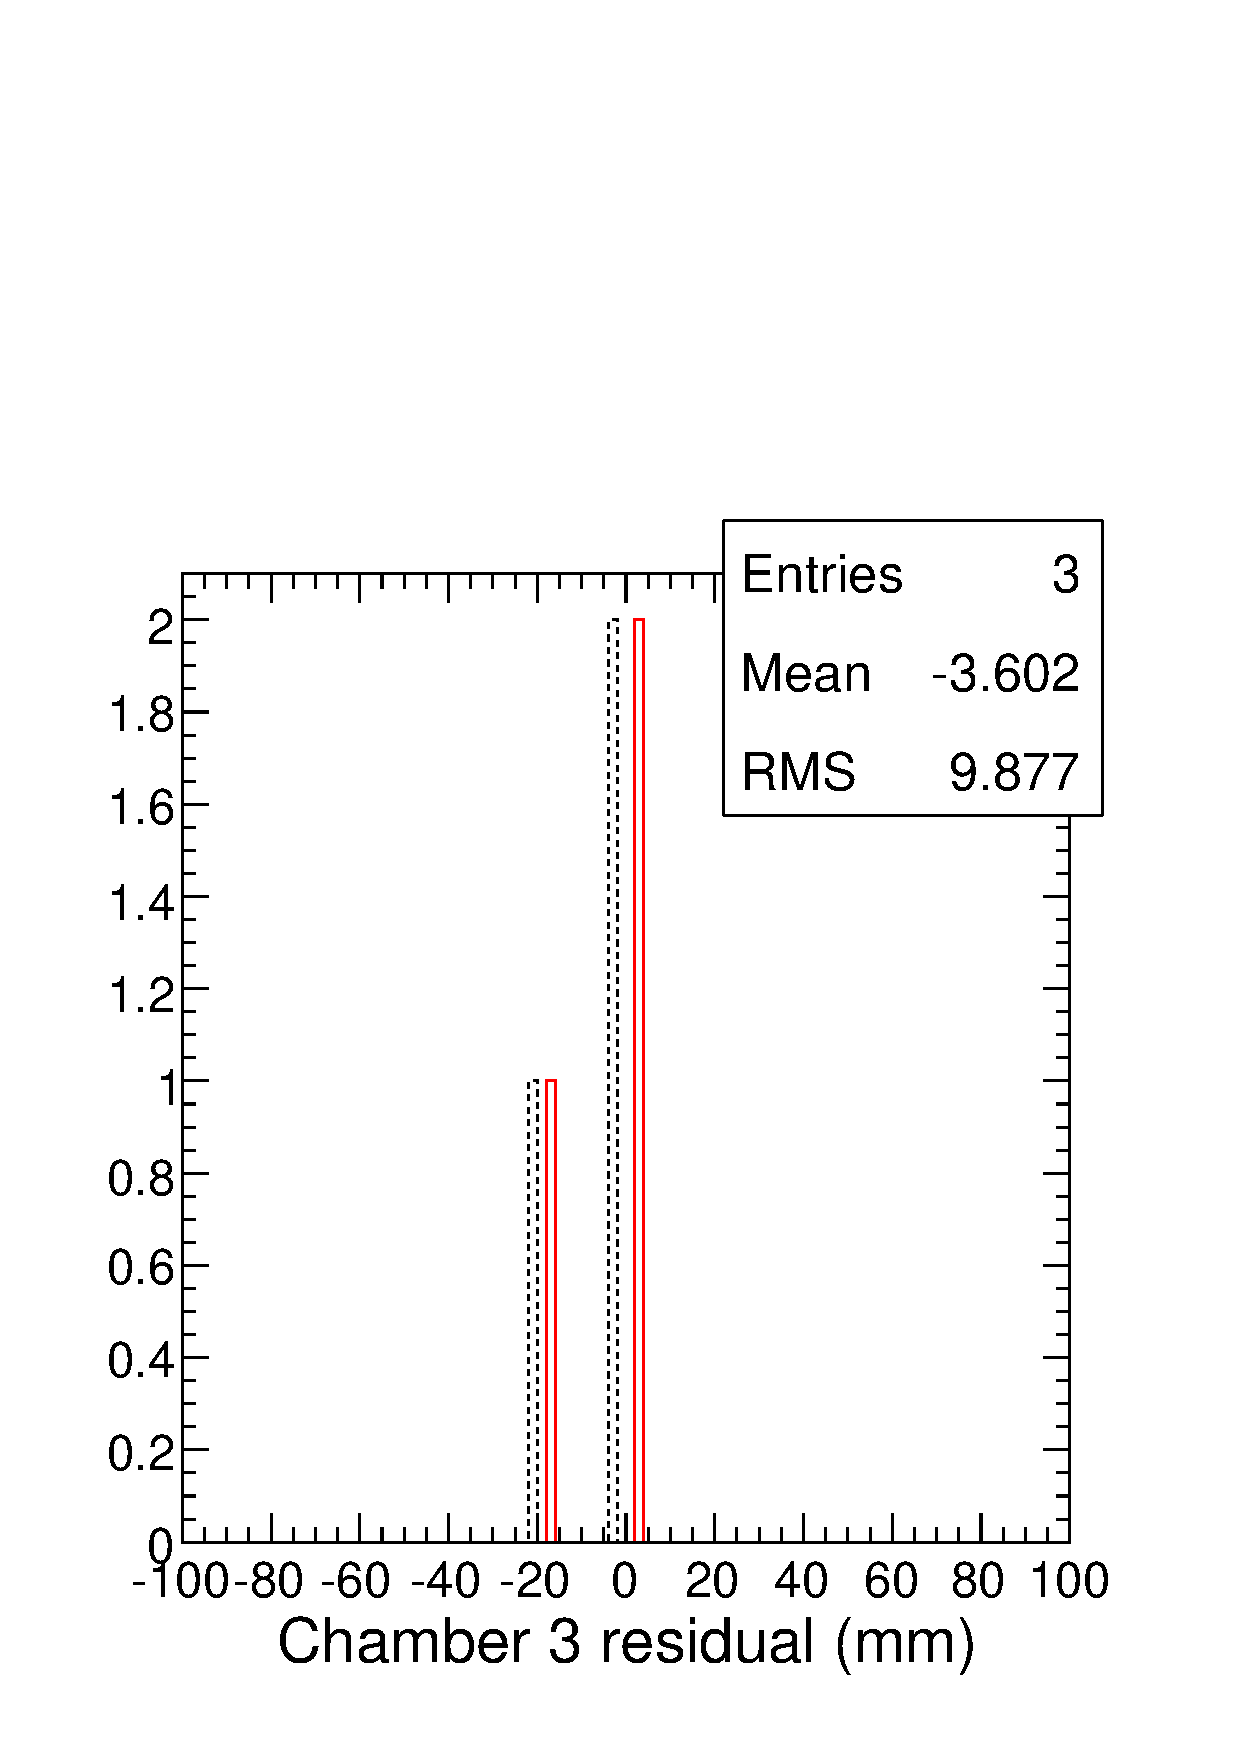
\includegraphics[width=0.11\linewidth]{endcap_mem22_3.pdf}
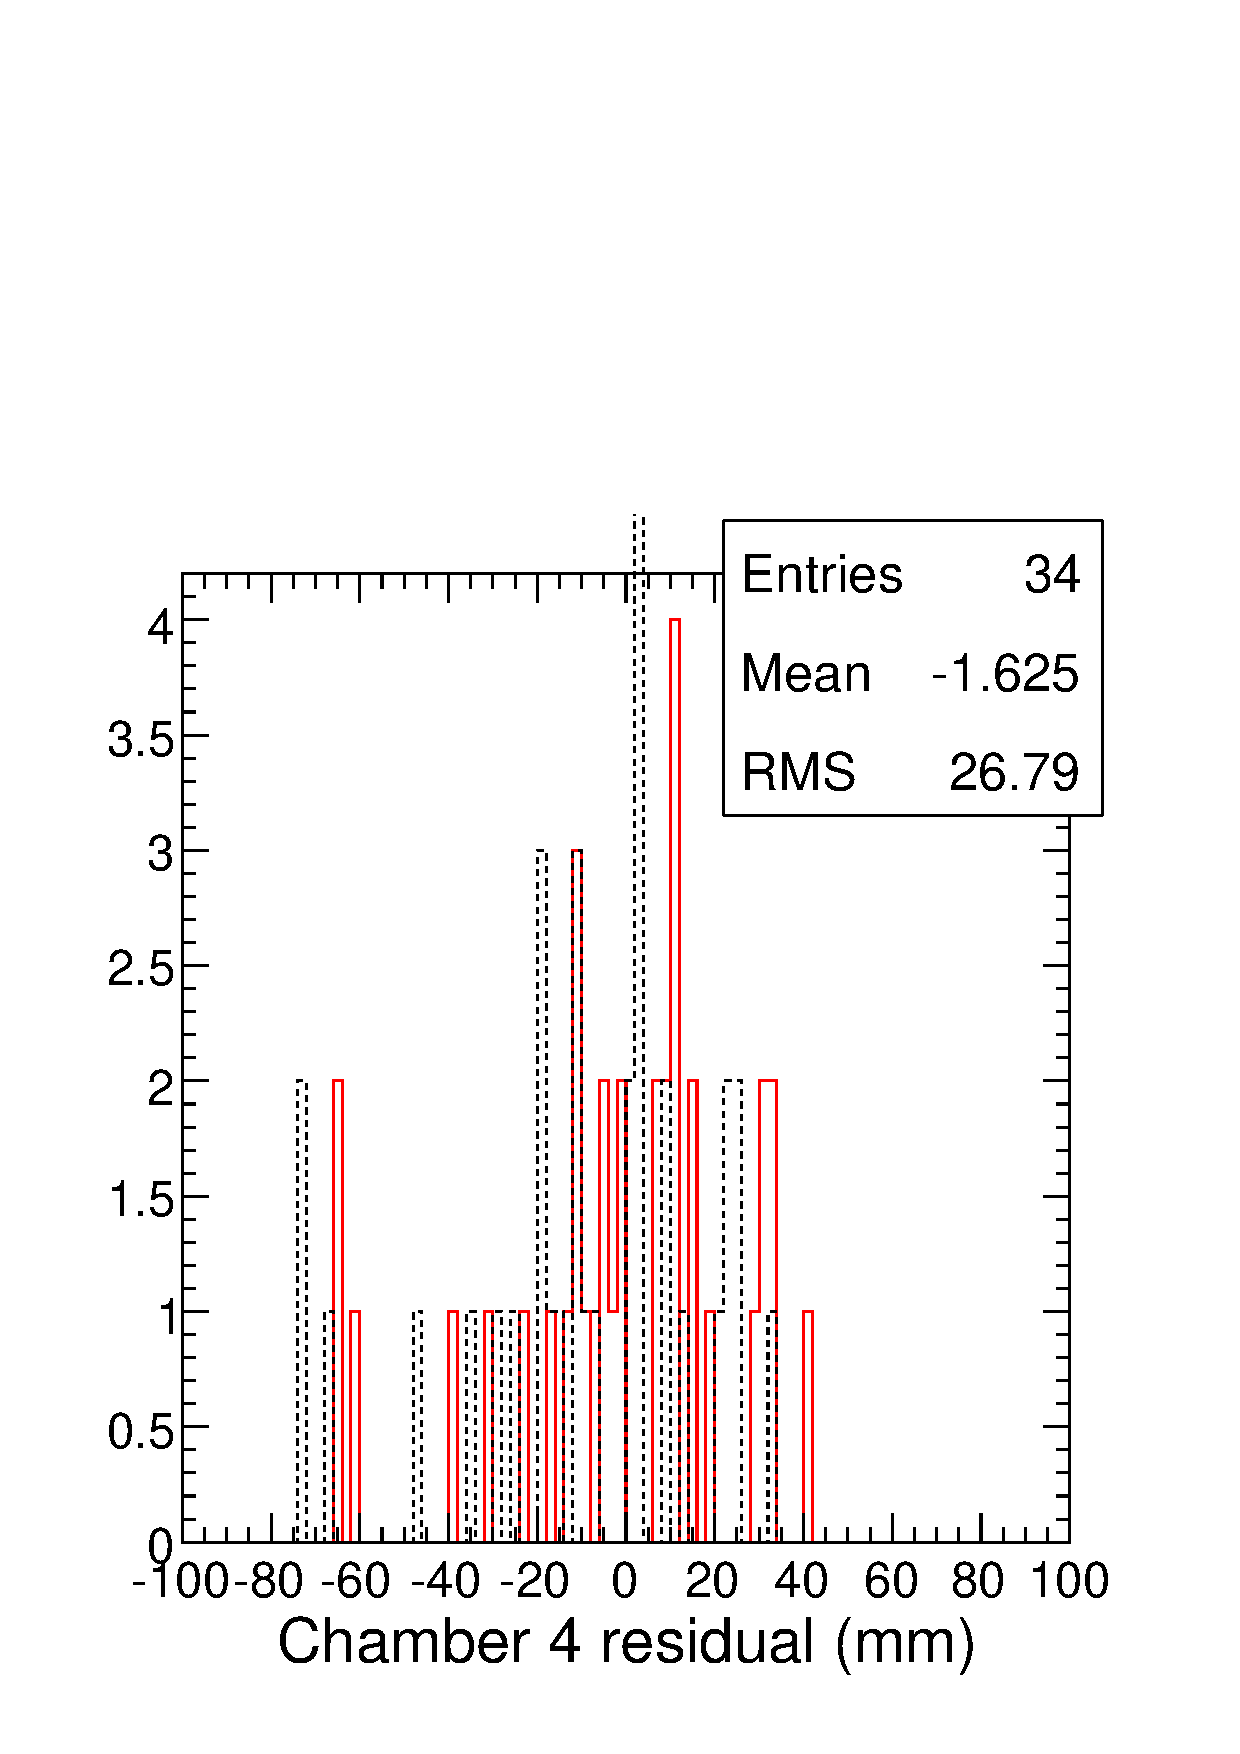
\includegraphics[width=0.11\linewidth]{endcap_mem22_4.pdf}
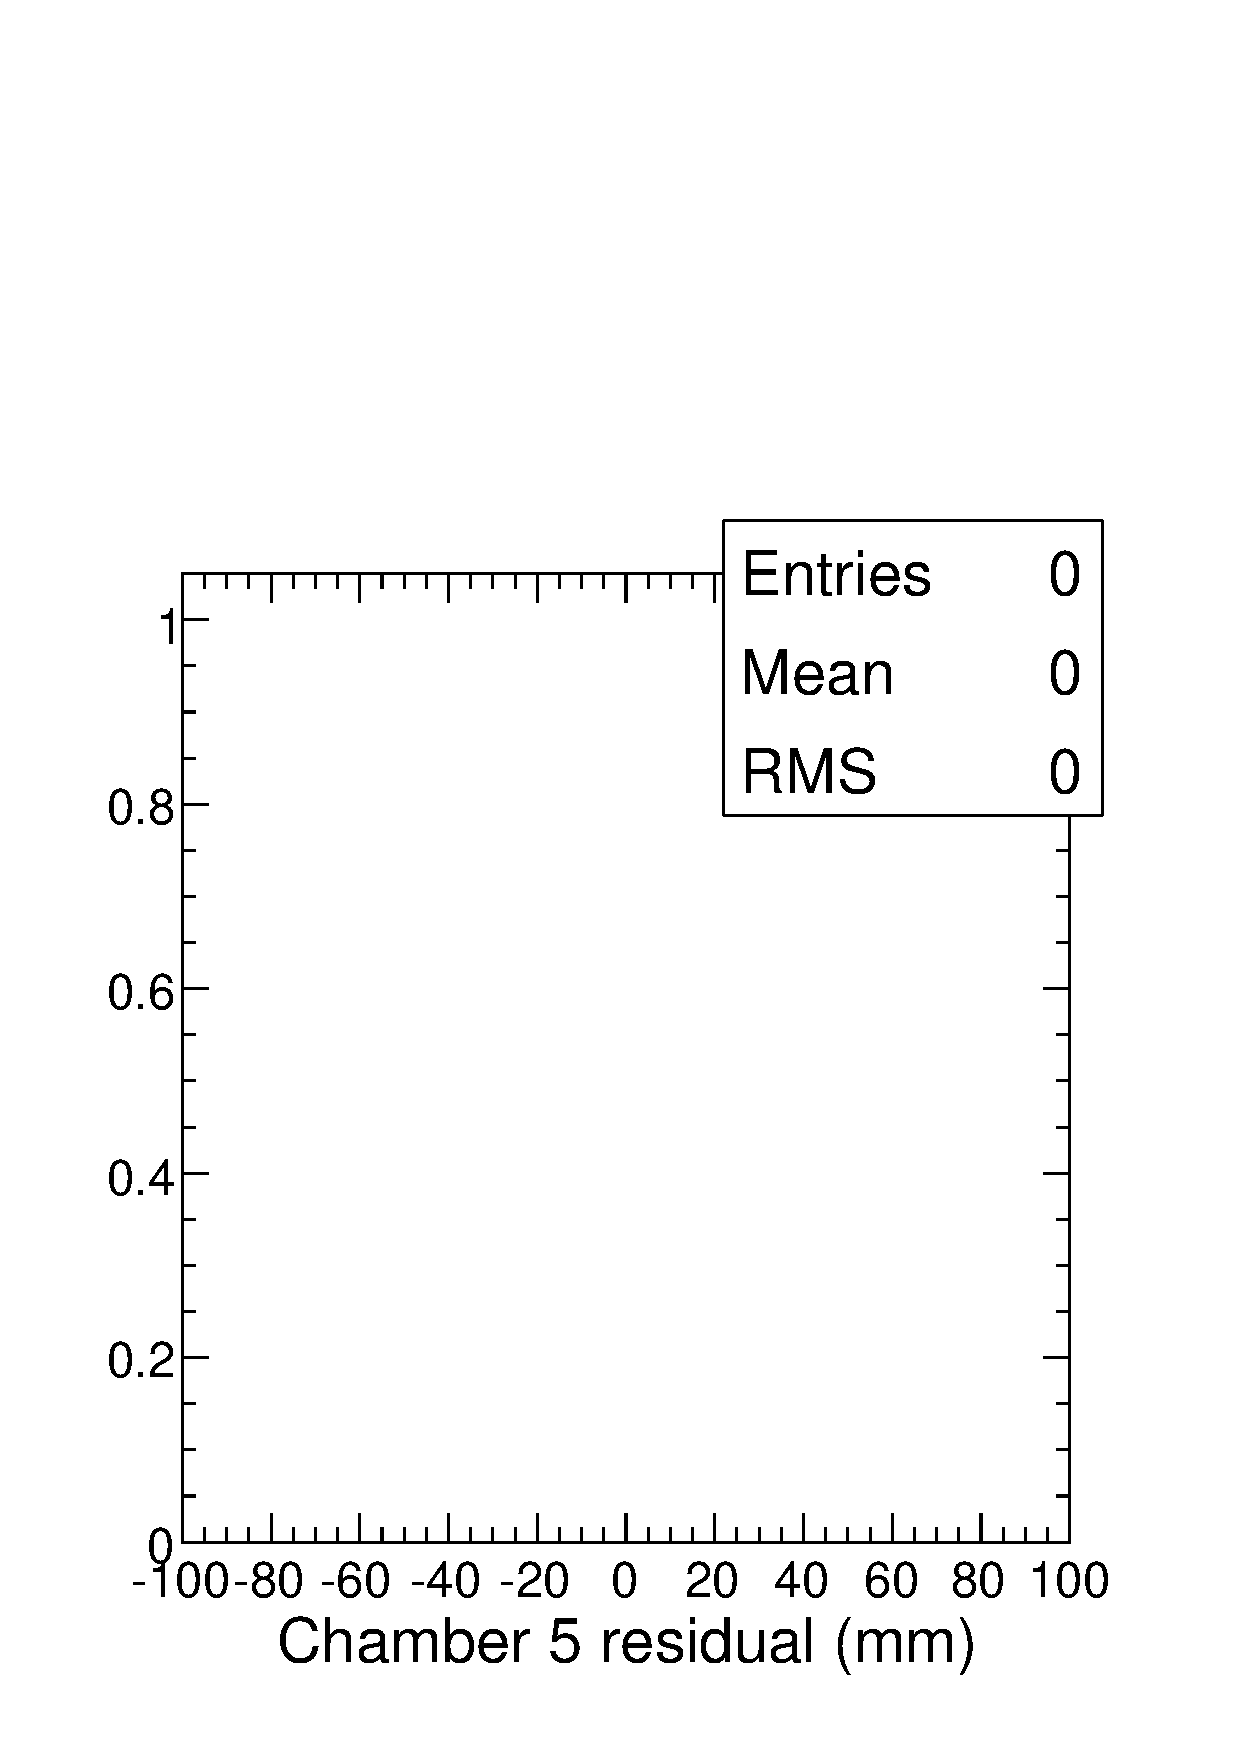
\includegraphics[width=0.11\linewidth]{endcap_mem22_5.pdf}
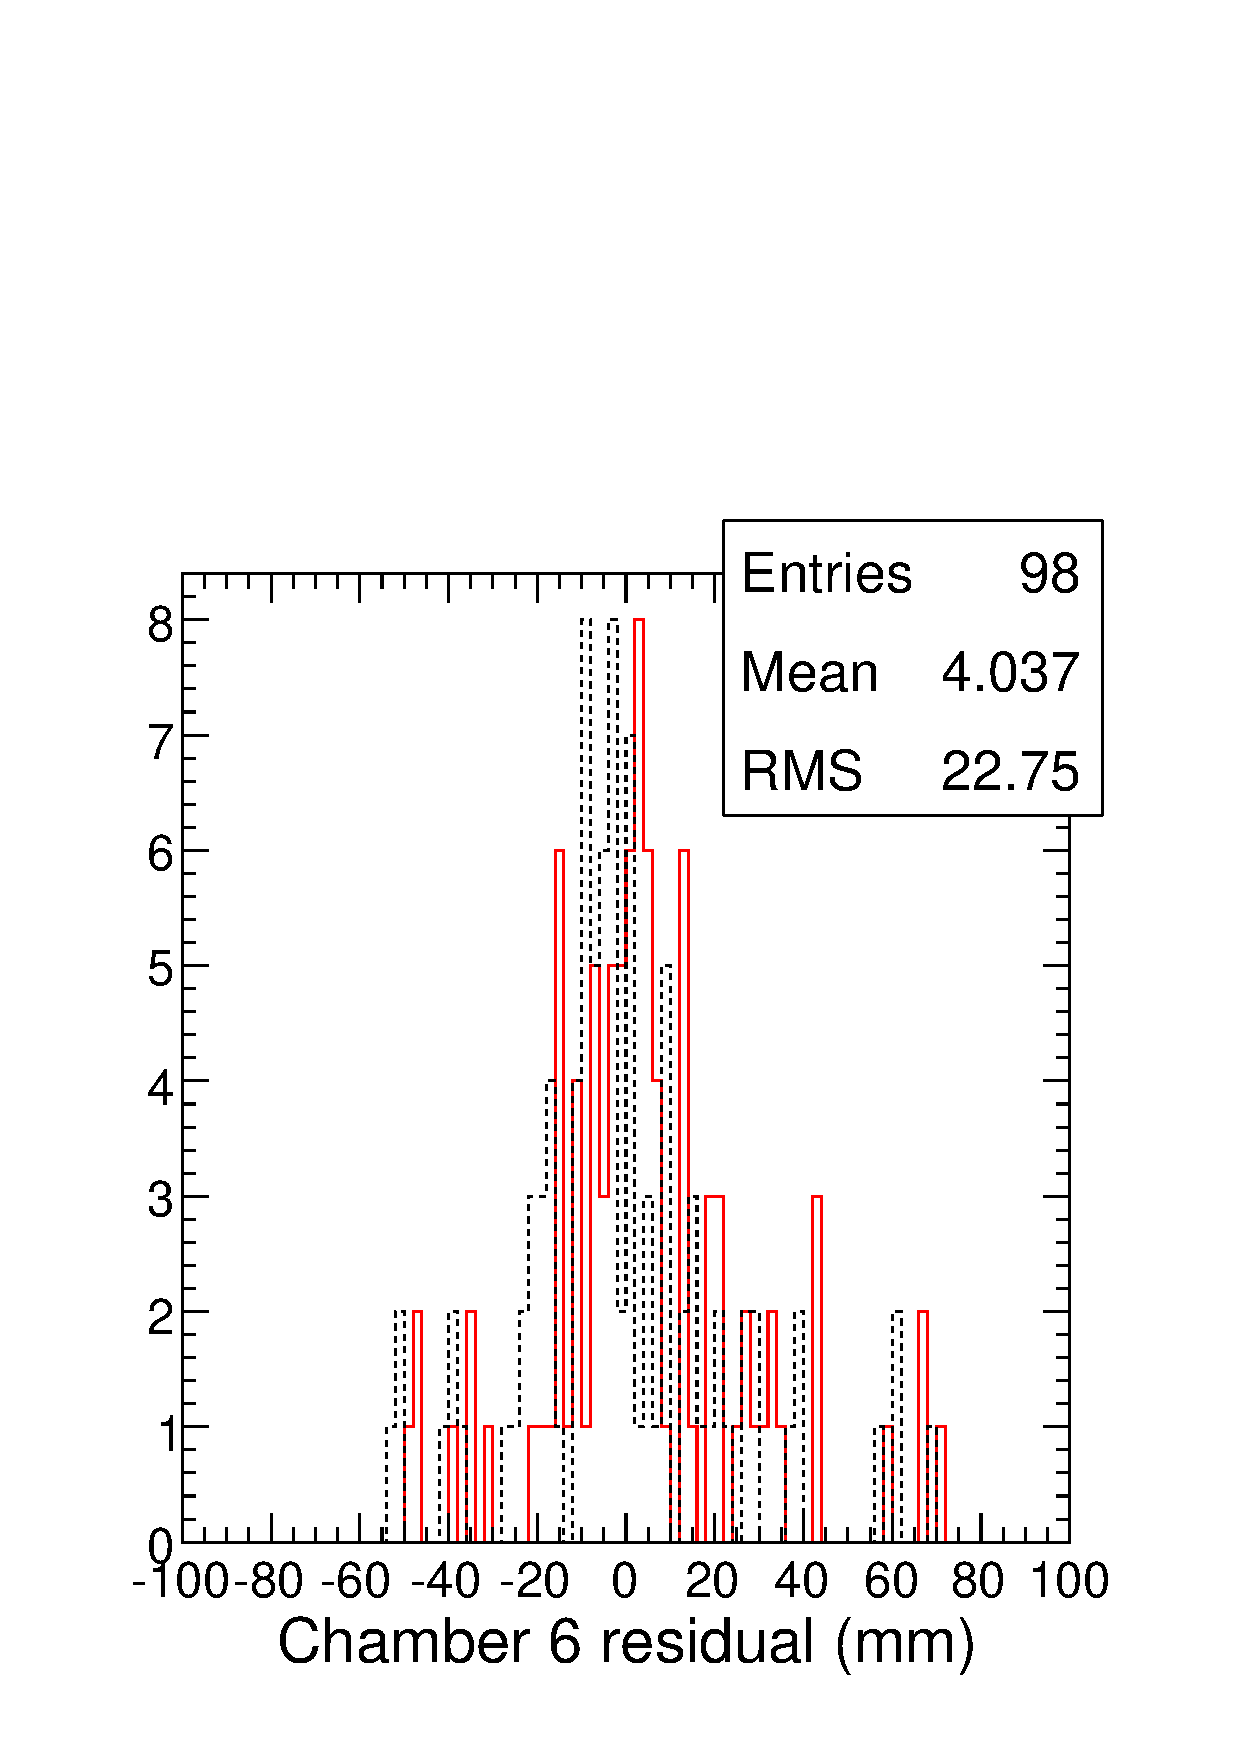
\includegraphics[width=0.11\linewidth]{endcap_mem22_6.pdf}
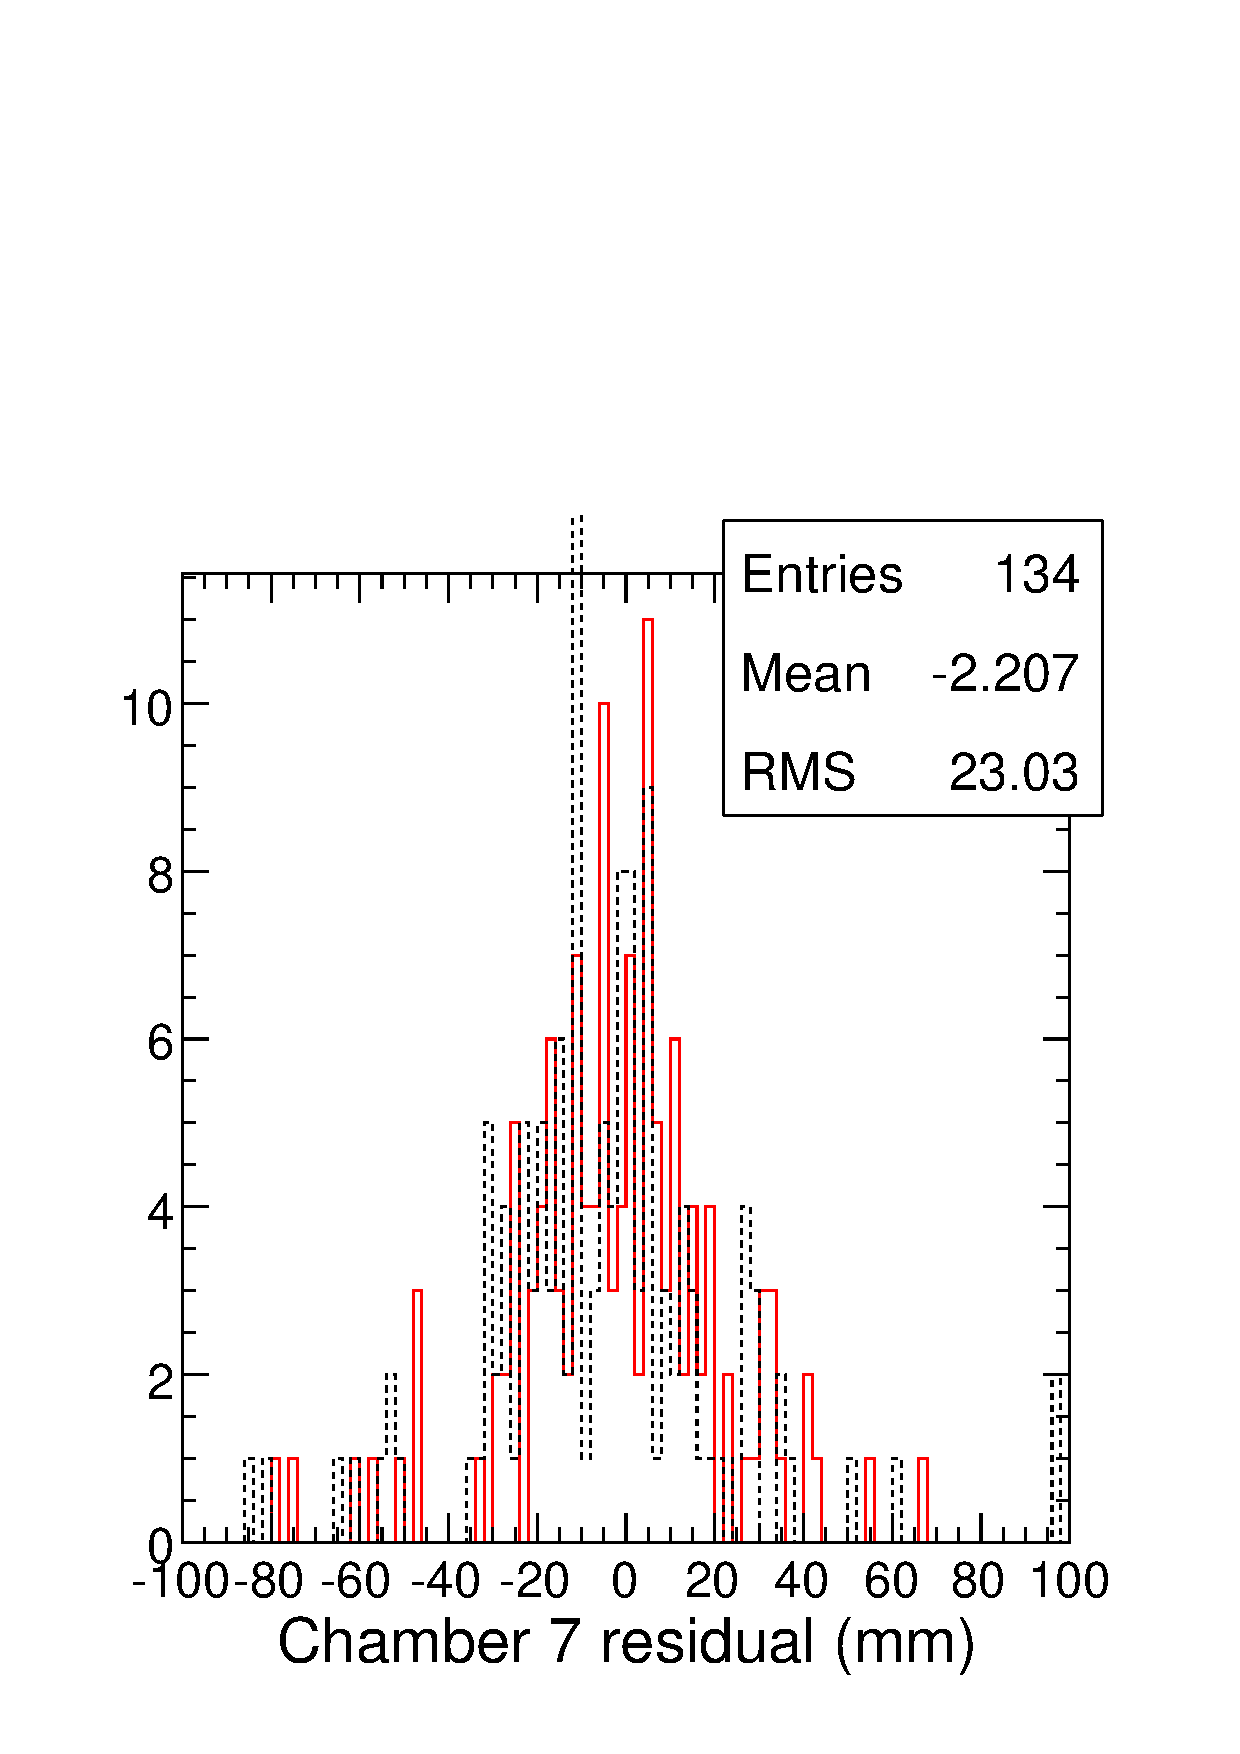
\includegraphics[width=0.11\linewidth]{endcap_mem22_7.pdf}
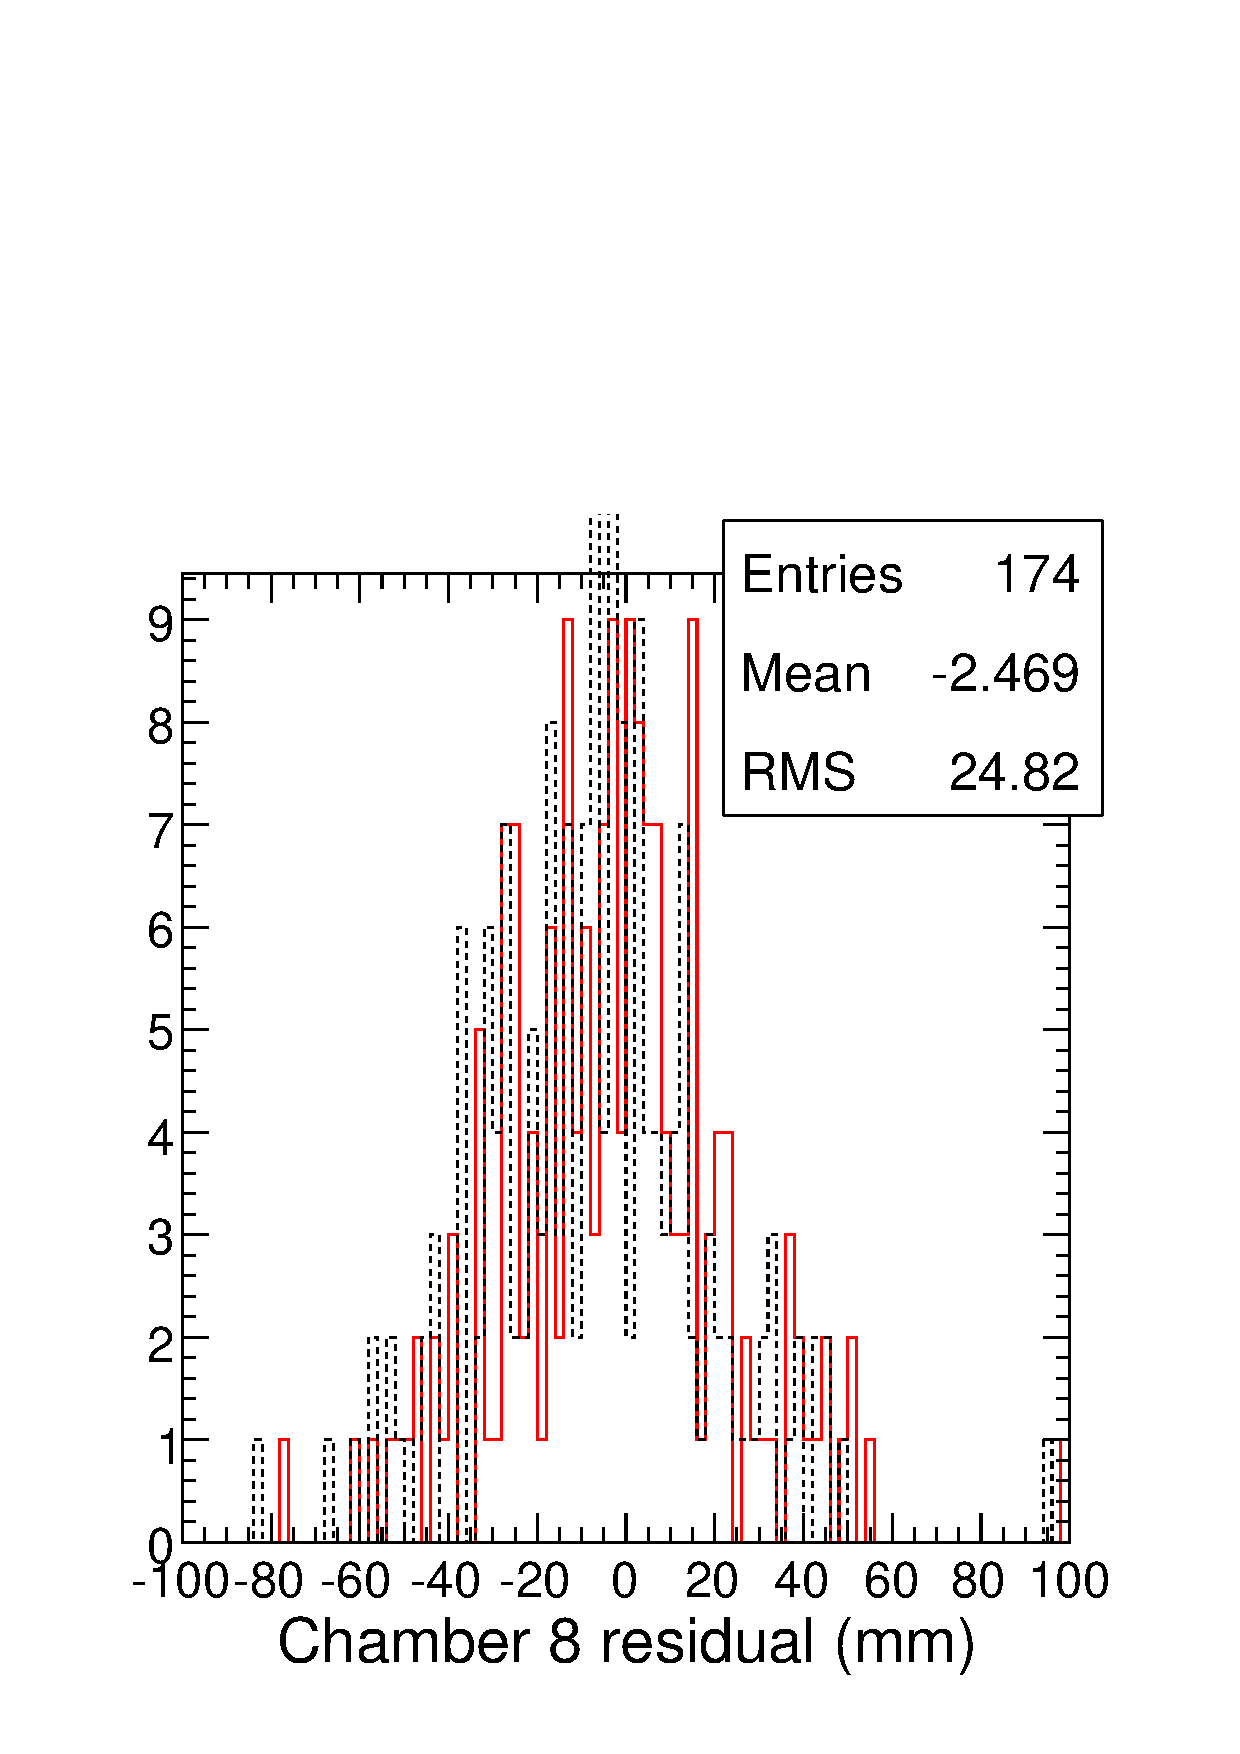
\includegraphics[width=0.11\linewidth]{endcap_mem22_8.pdf}
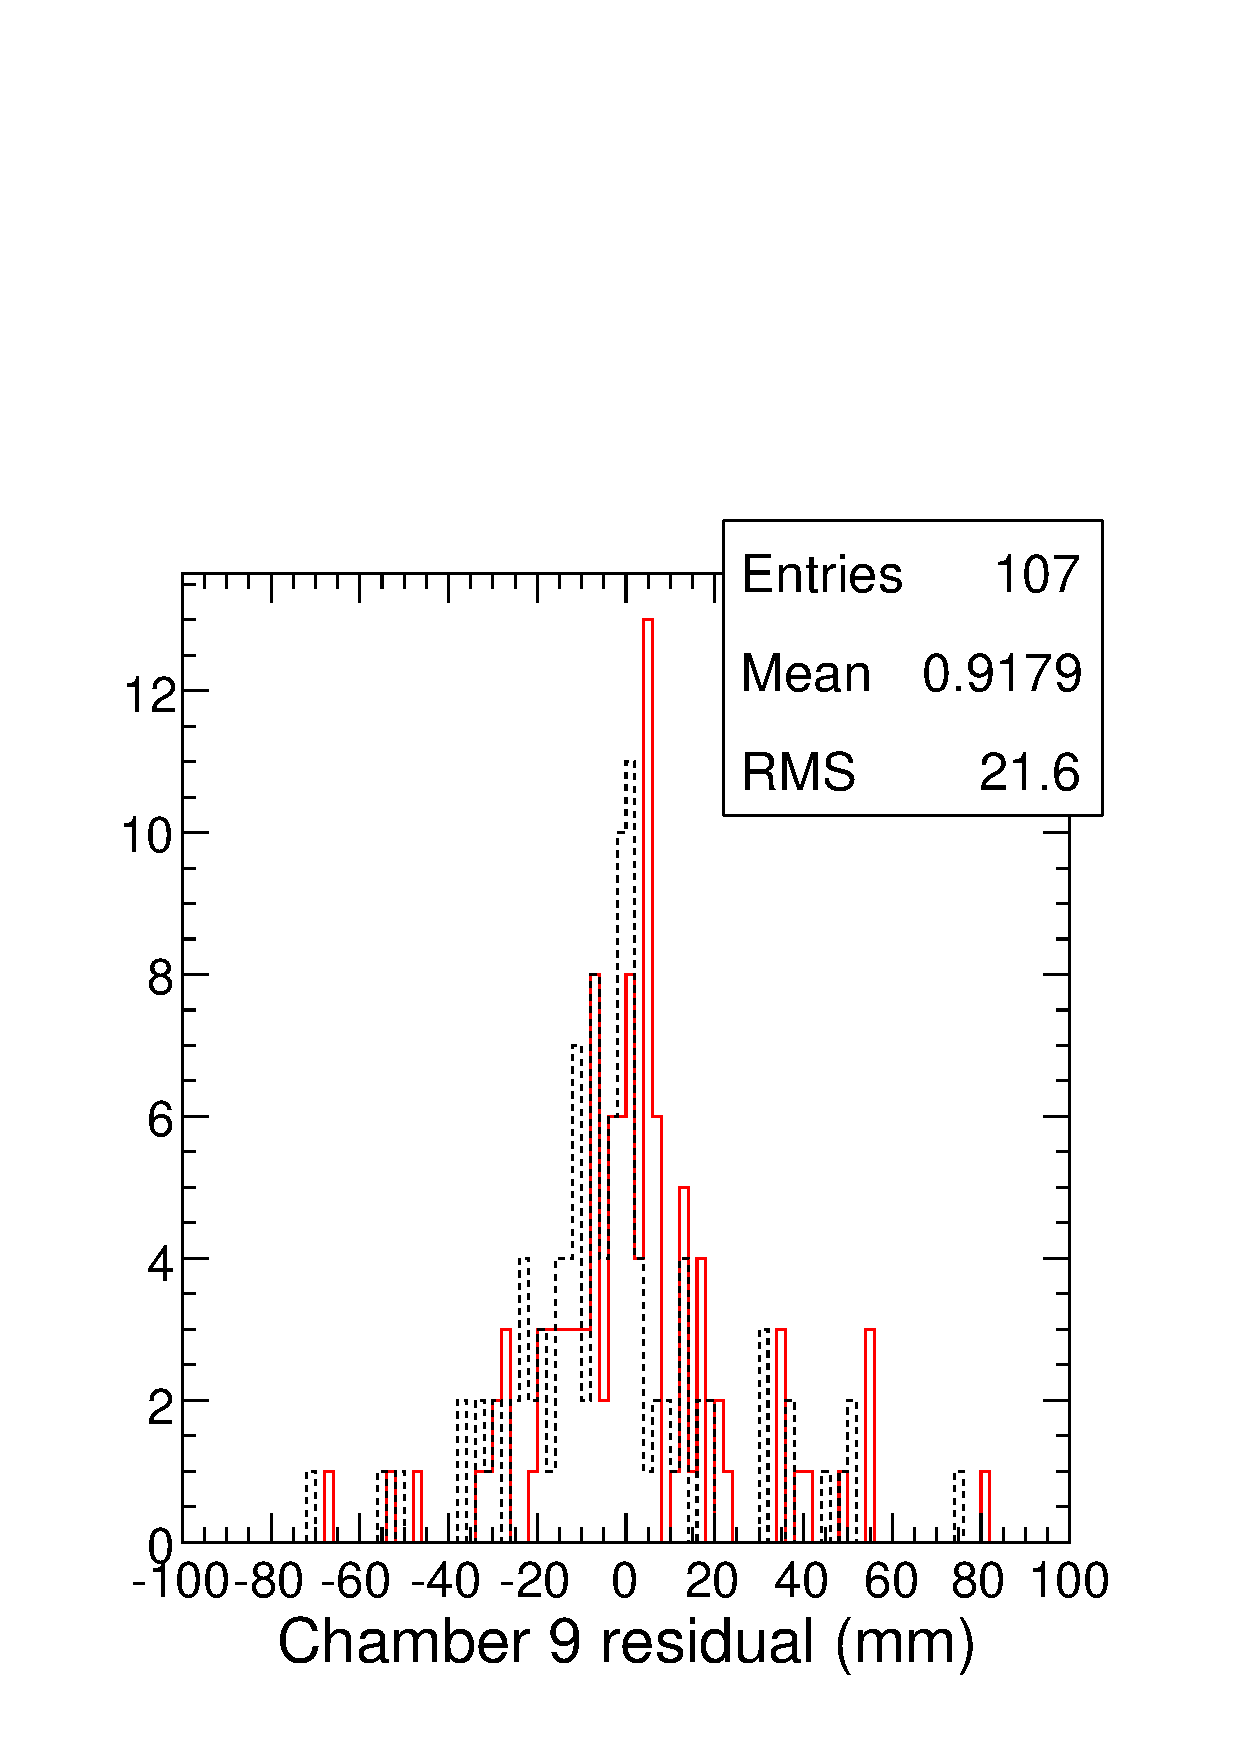
\includegraphics[width=0.11\linewidth]{endcap_mem22_9.pdf}

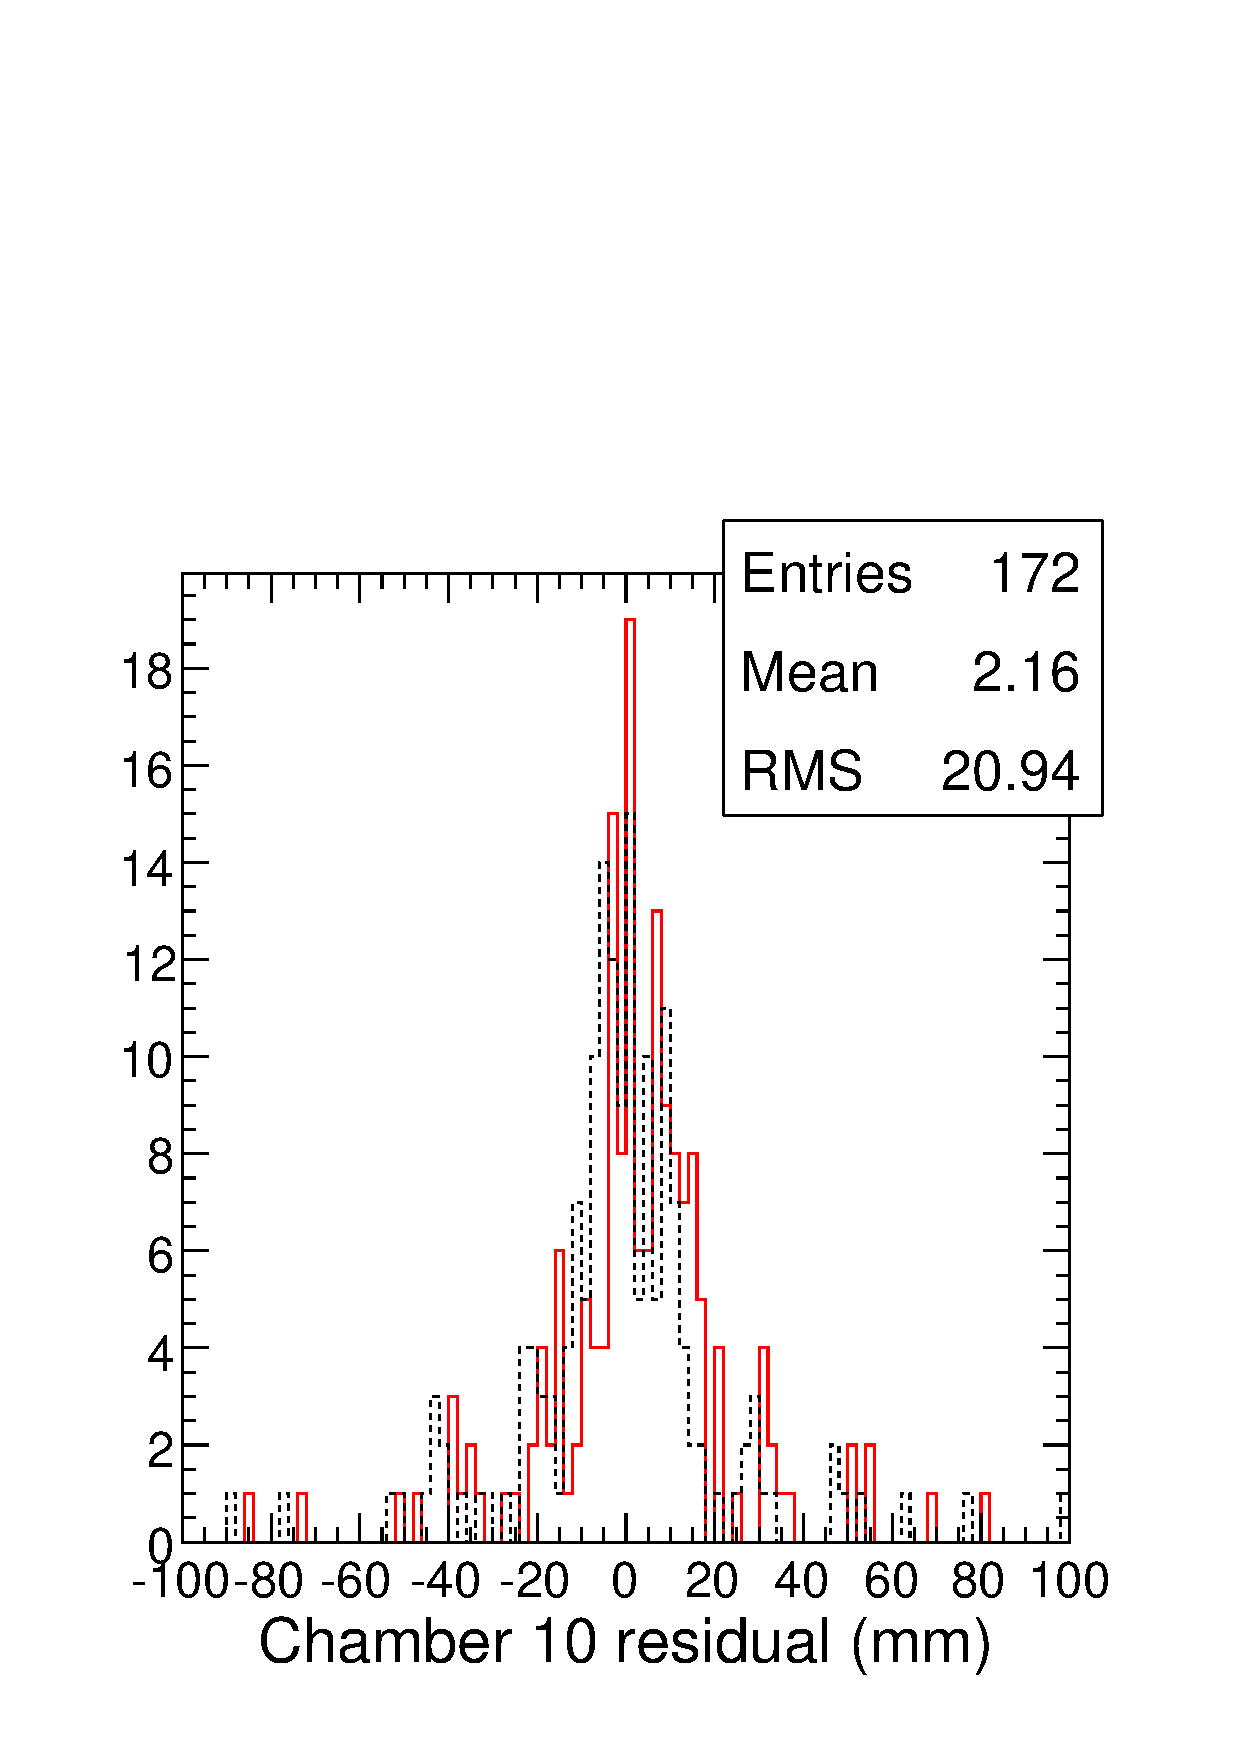
\includegraphics[width=0.11\linewidth]{endcap_mem22_10.pdf}
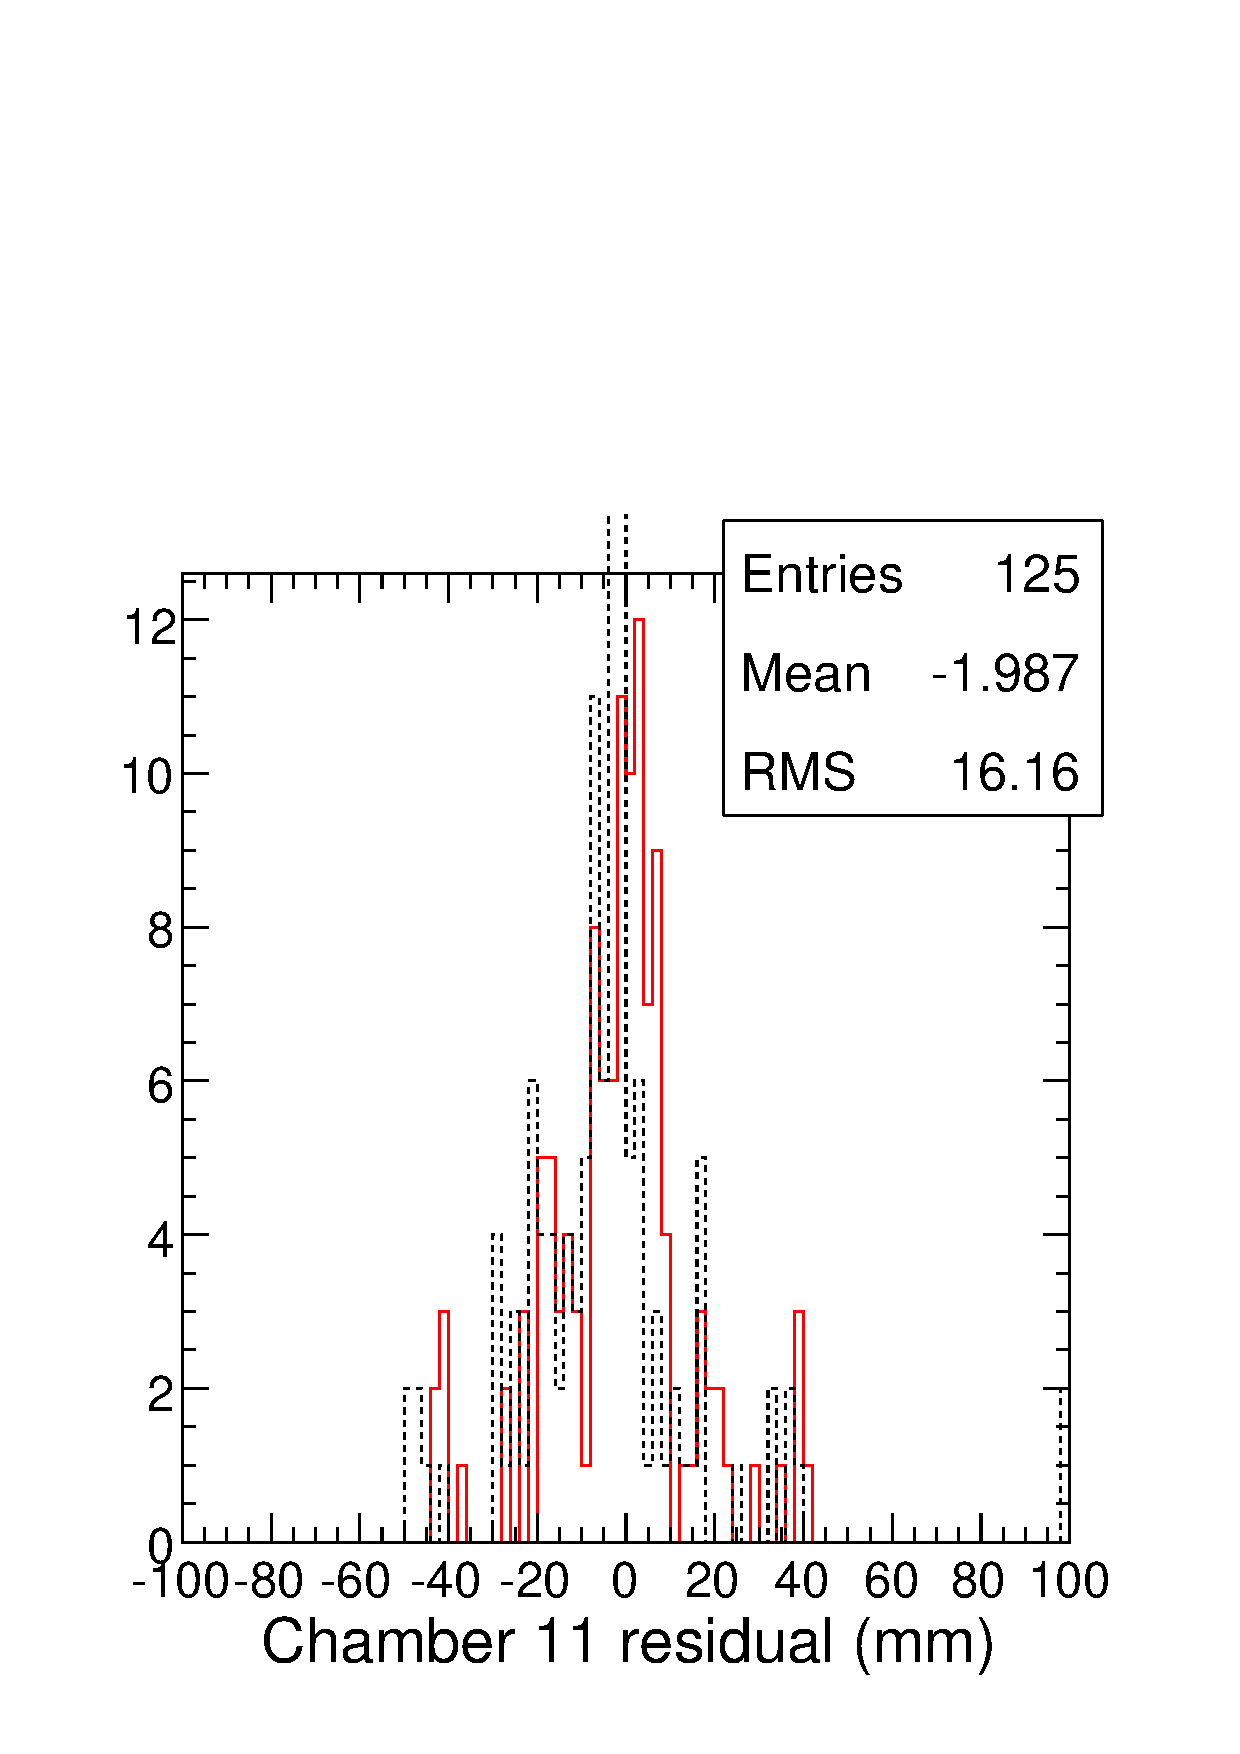
\includegraphics[width=0.11\linewidth]{endcap_mem22_11.pdf}
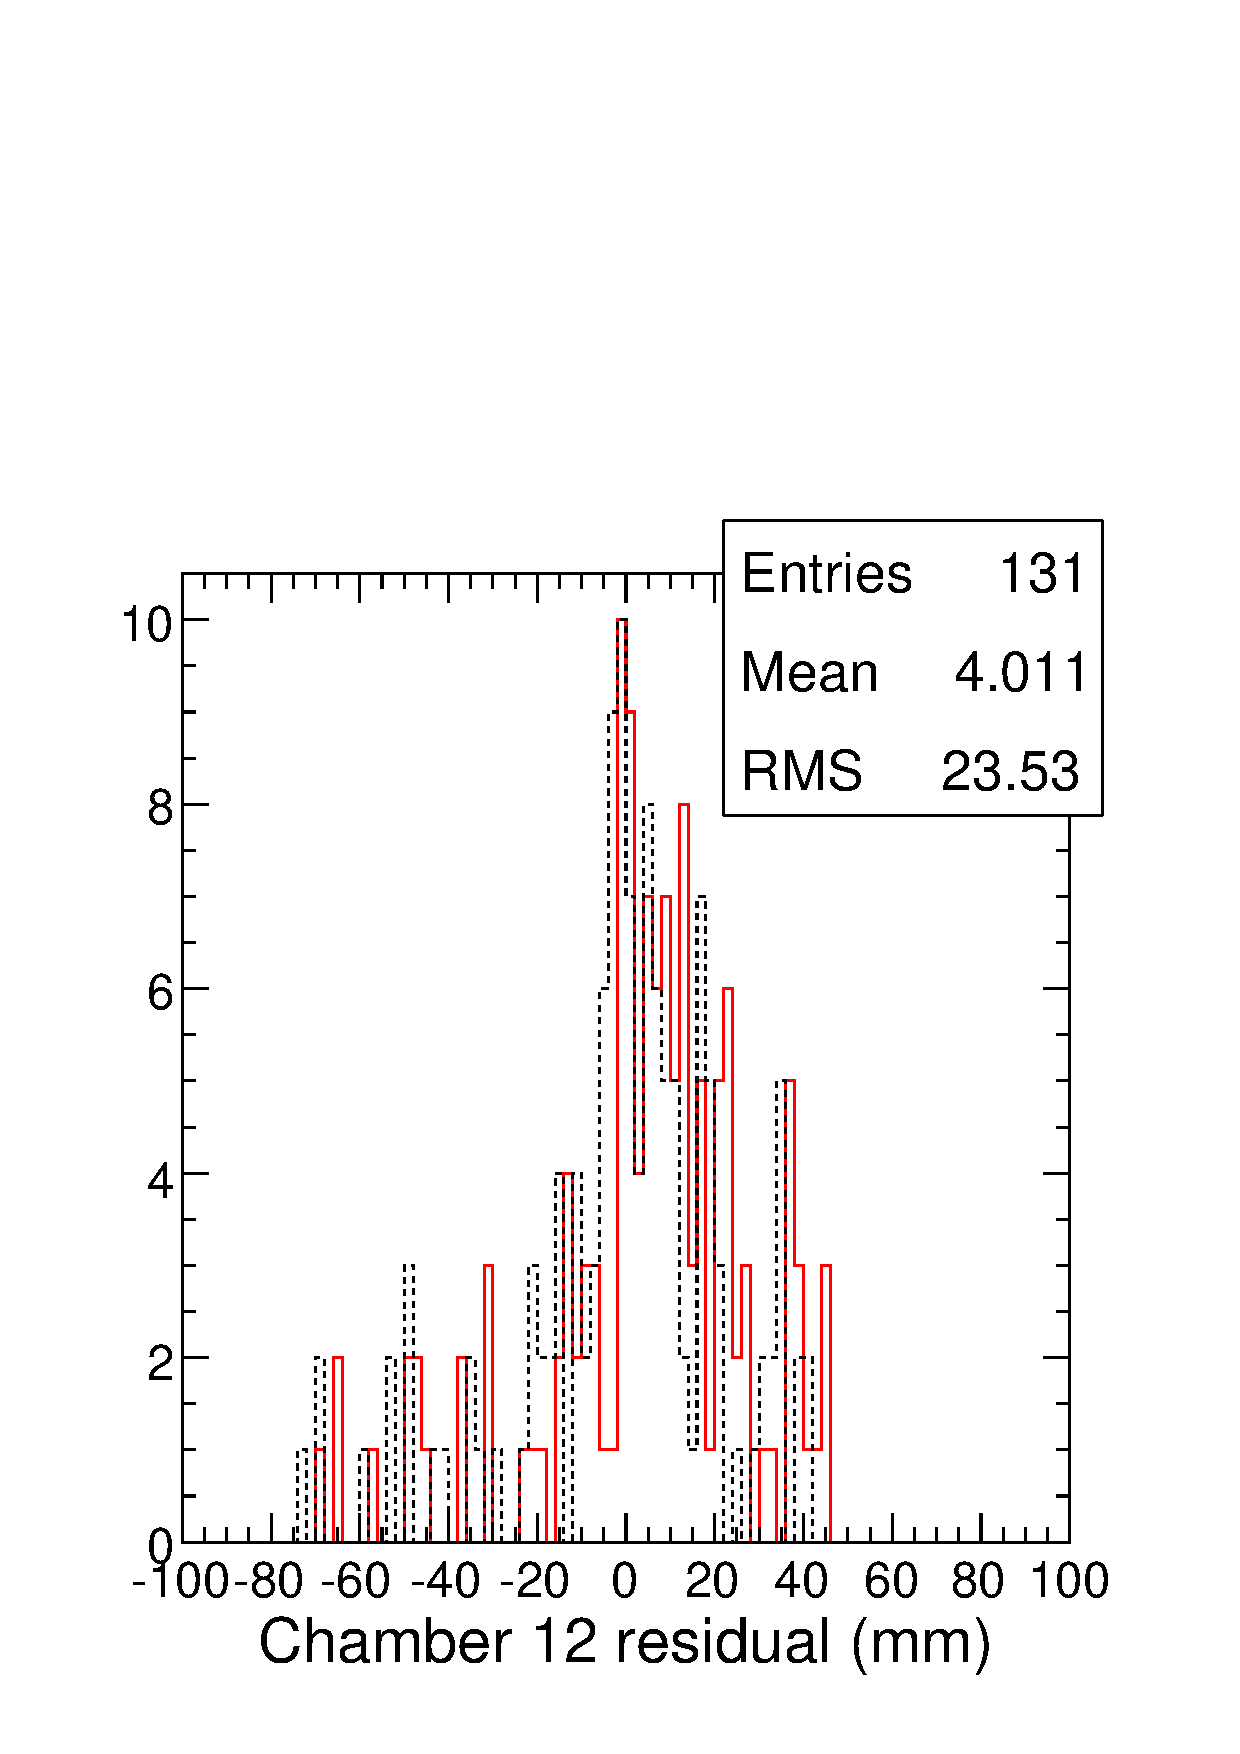
\includegraphics[width=0.11\linewidth]{endcap_mem22_12.pdf}
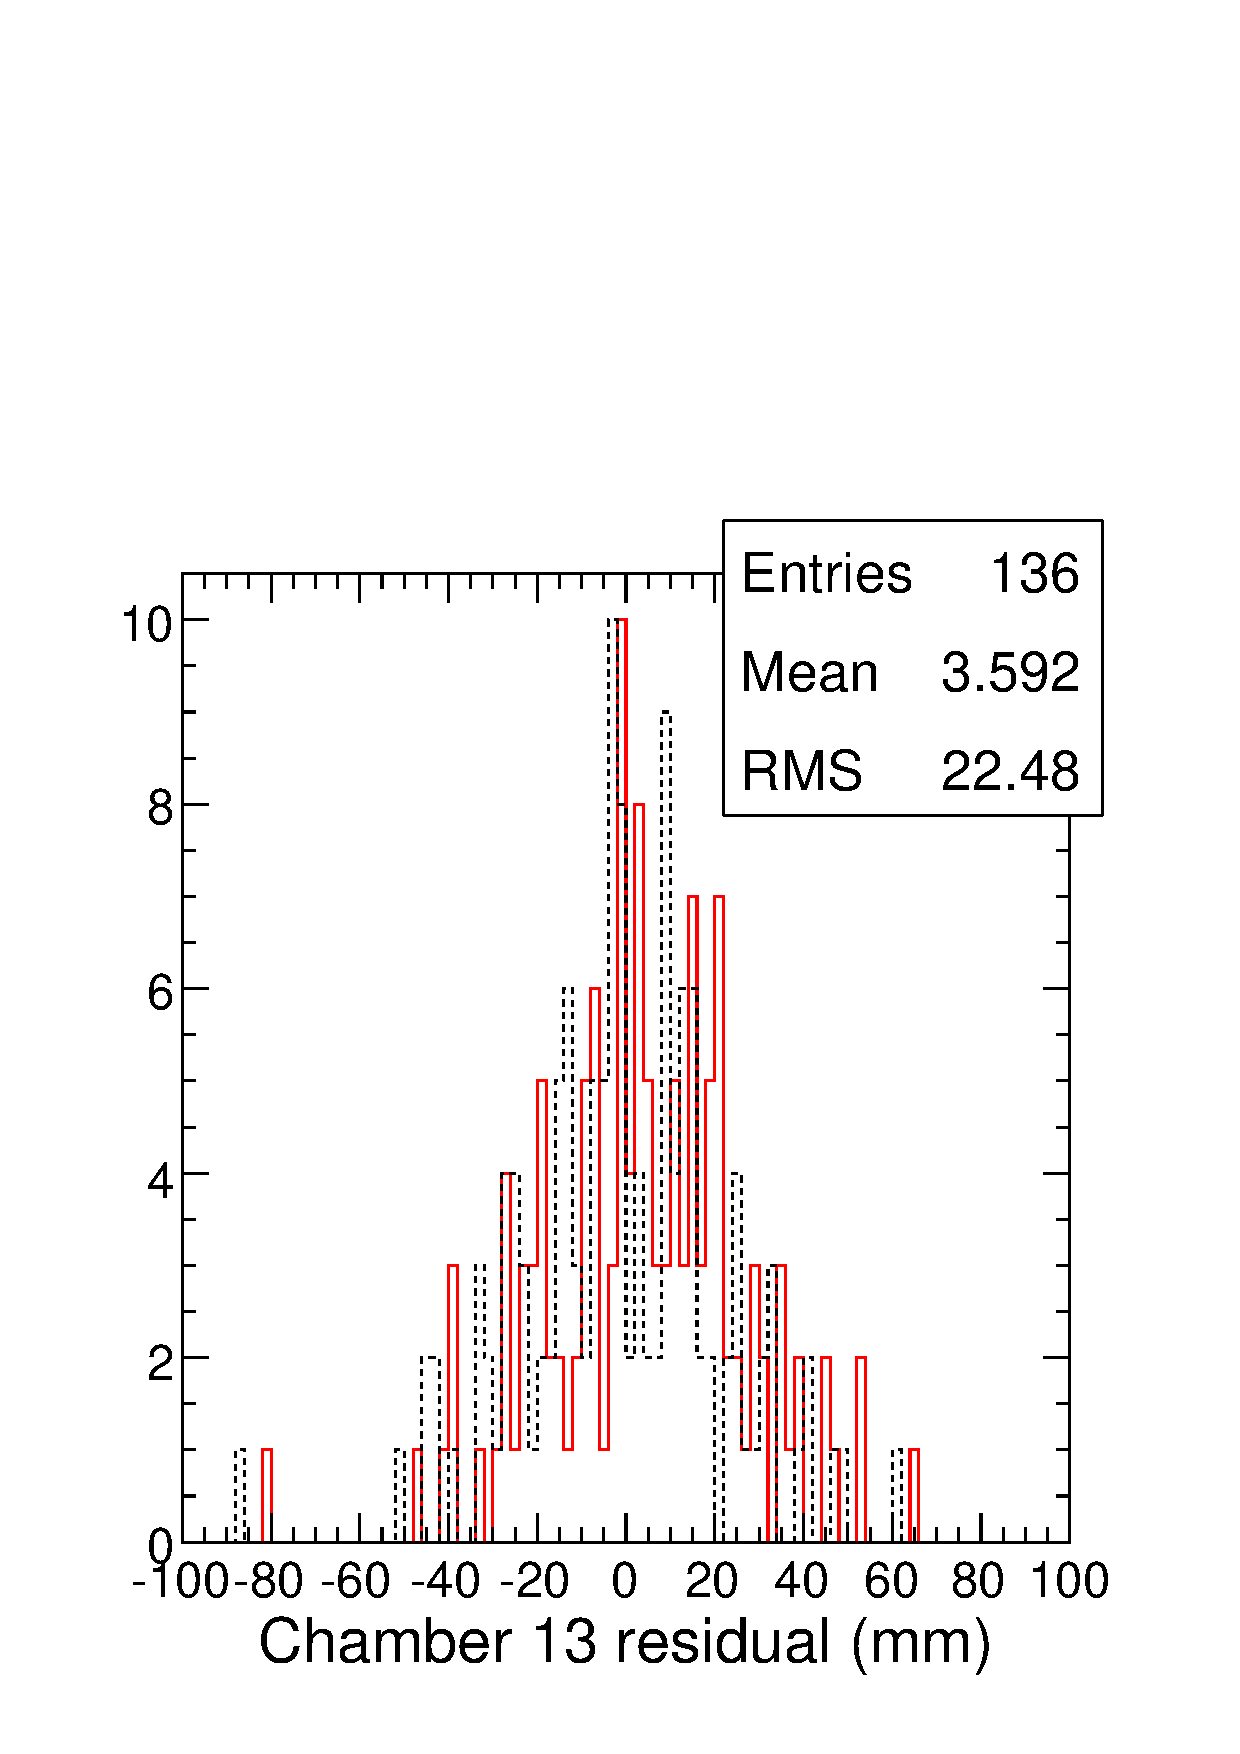
\includegraphics[width=0.11\linewidth]{endcap_mem22_13.pdf}
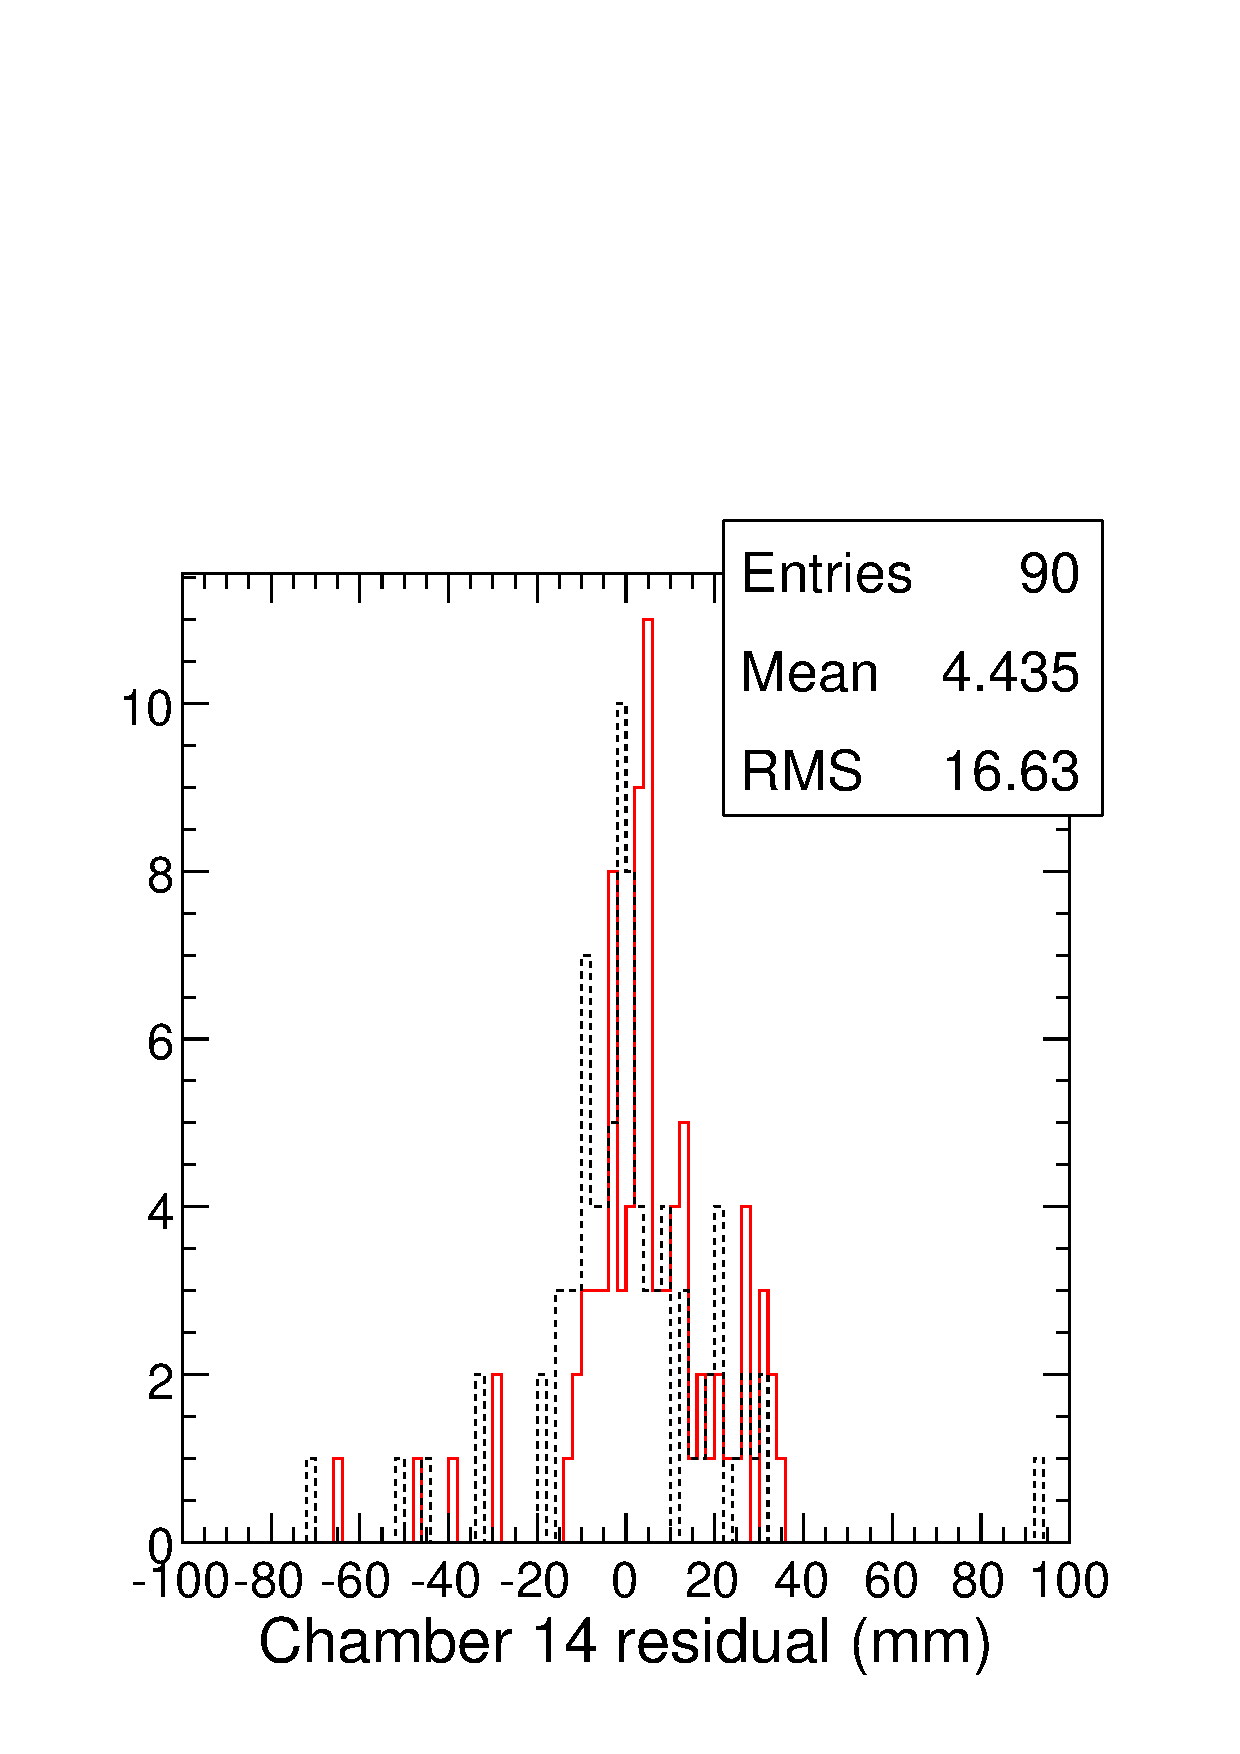
\includegraphics[width=0.11\linewidth]{endcap_mem22_14.pdf}
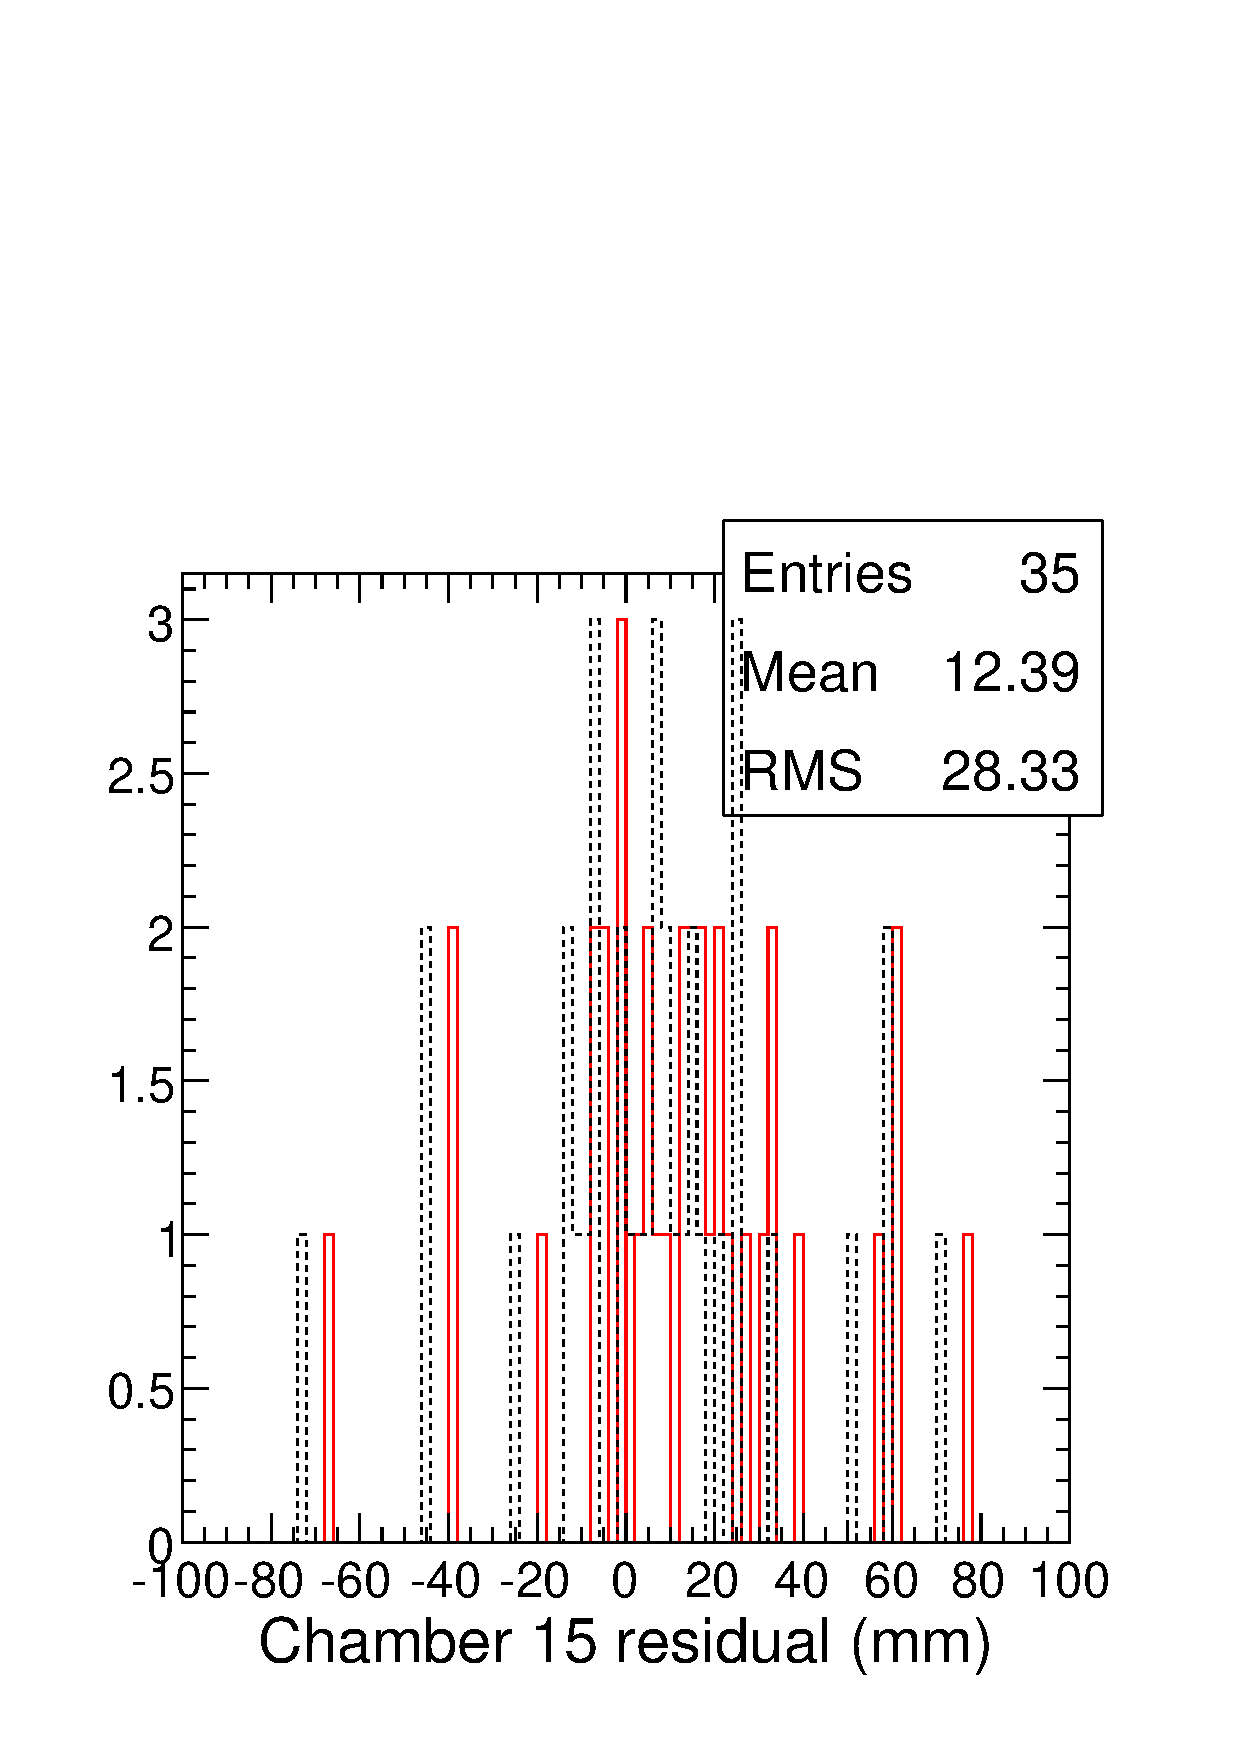
\includegraphics[width=0.11\linewidth]{endcap_mem22_15.pdf}
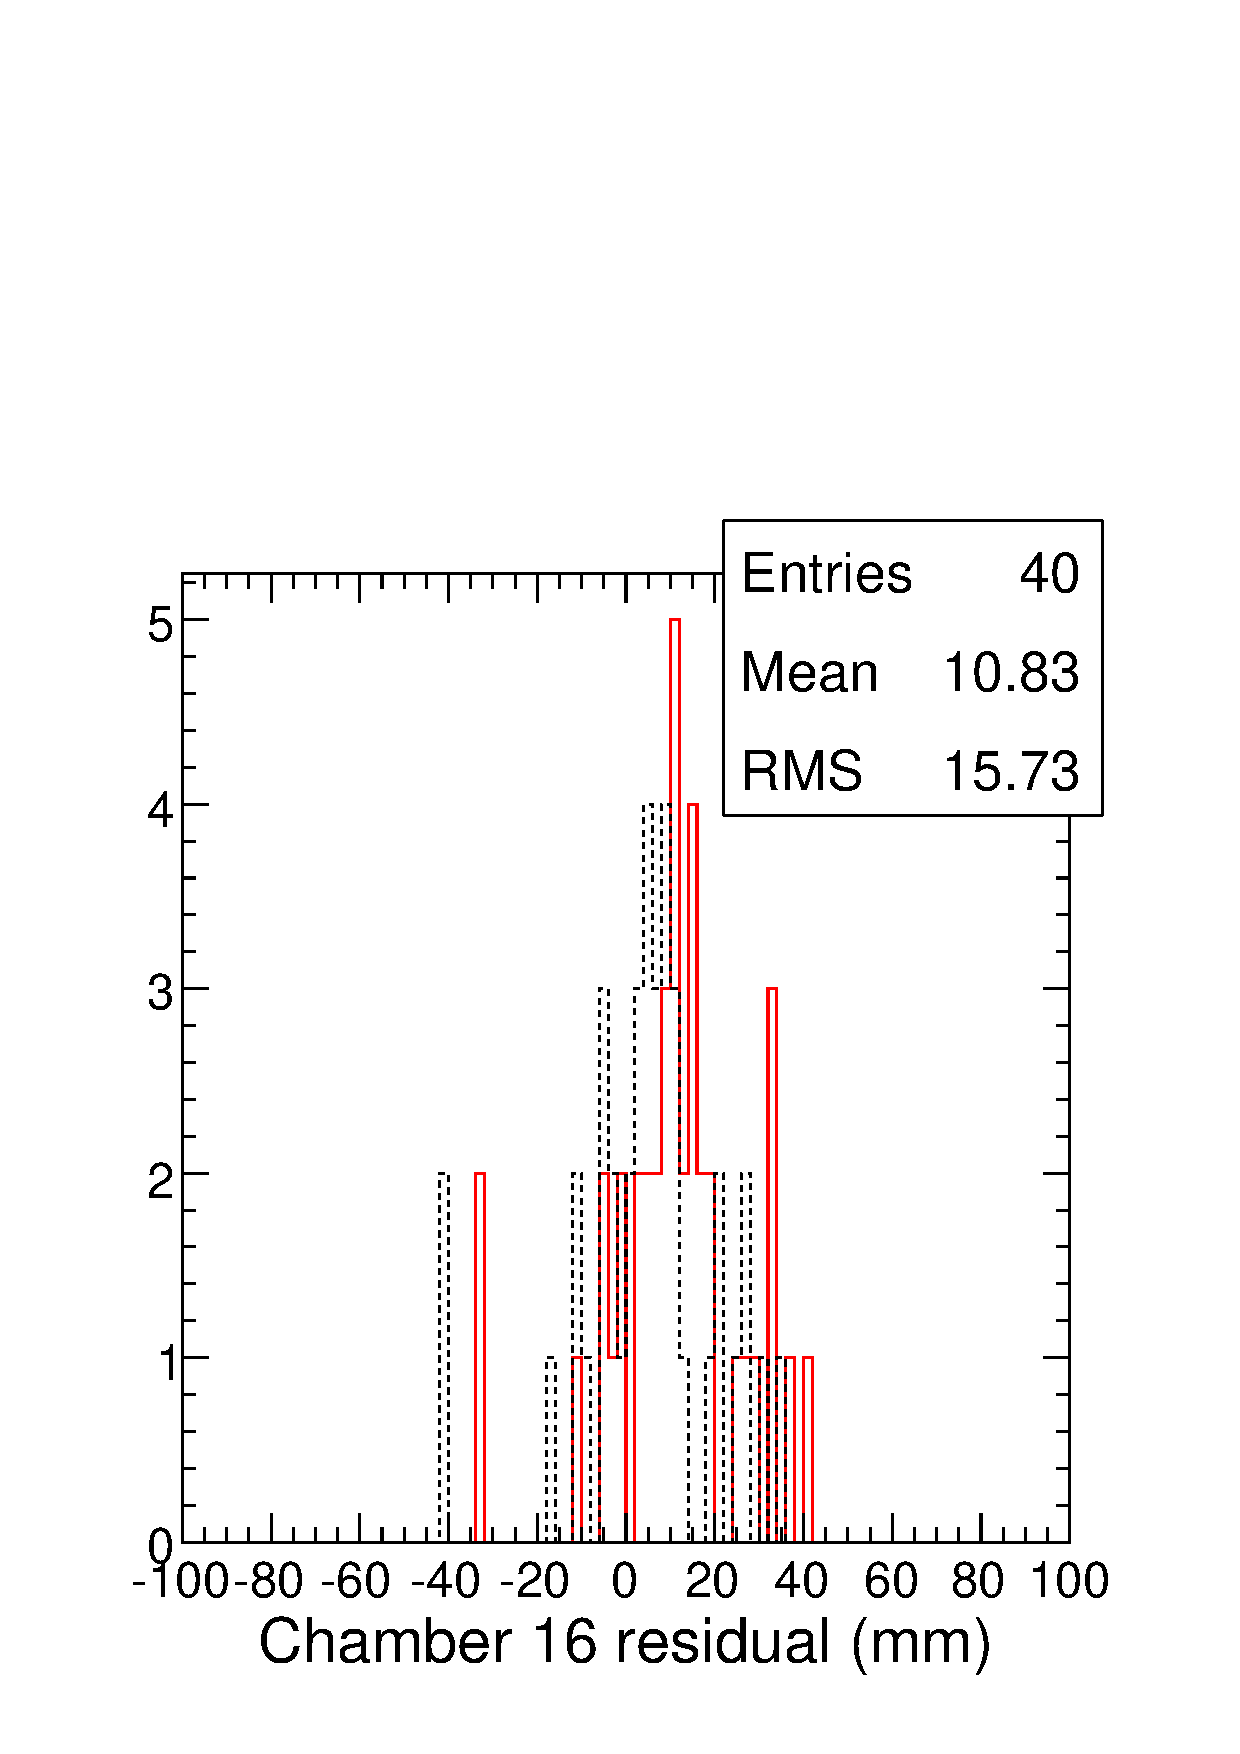
\includegraphics[width=0.11\linewidth]{endcap_mem22_16.pdf}
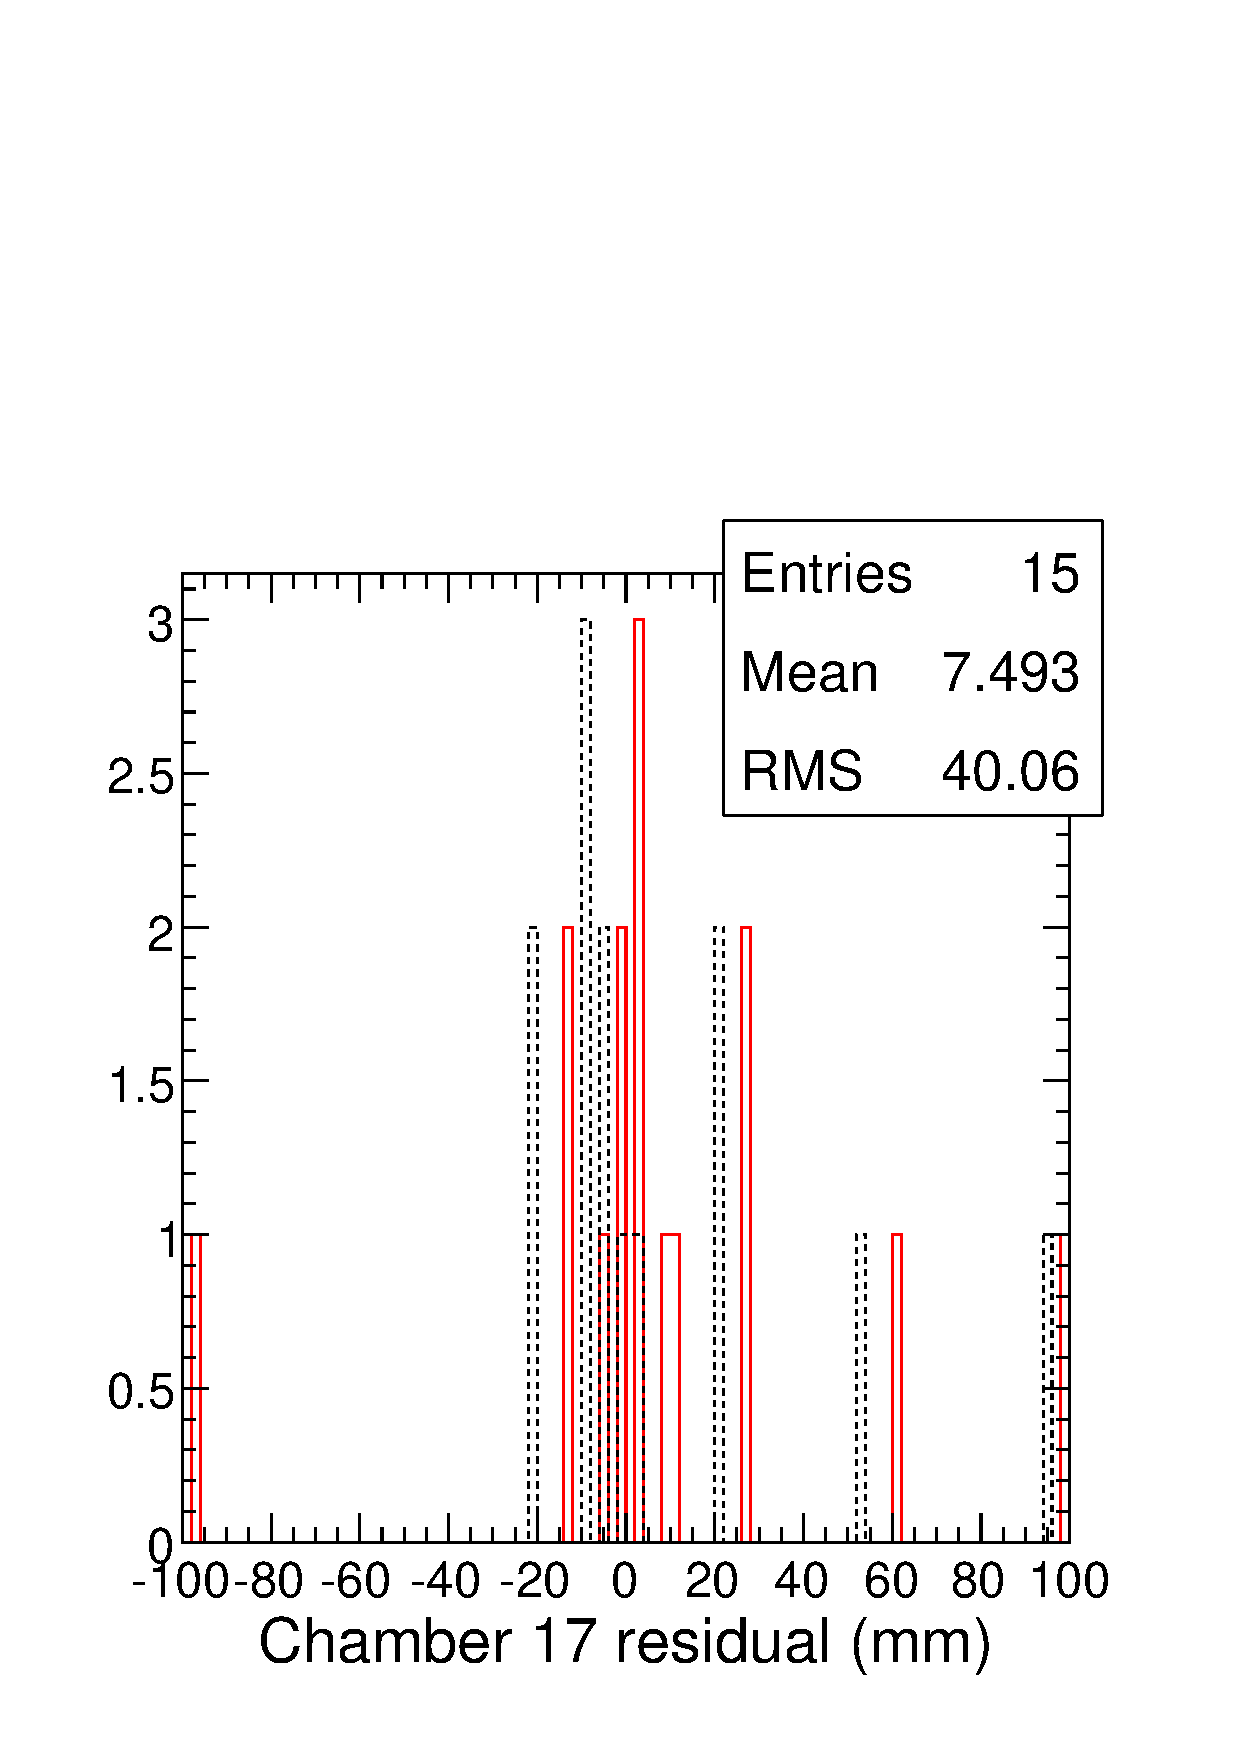
\includegraphics[width=0.11\linewidth]{endcap_mem22_17.pdf}
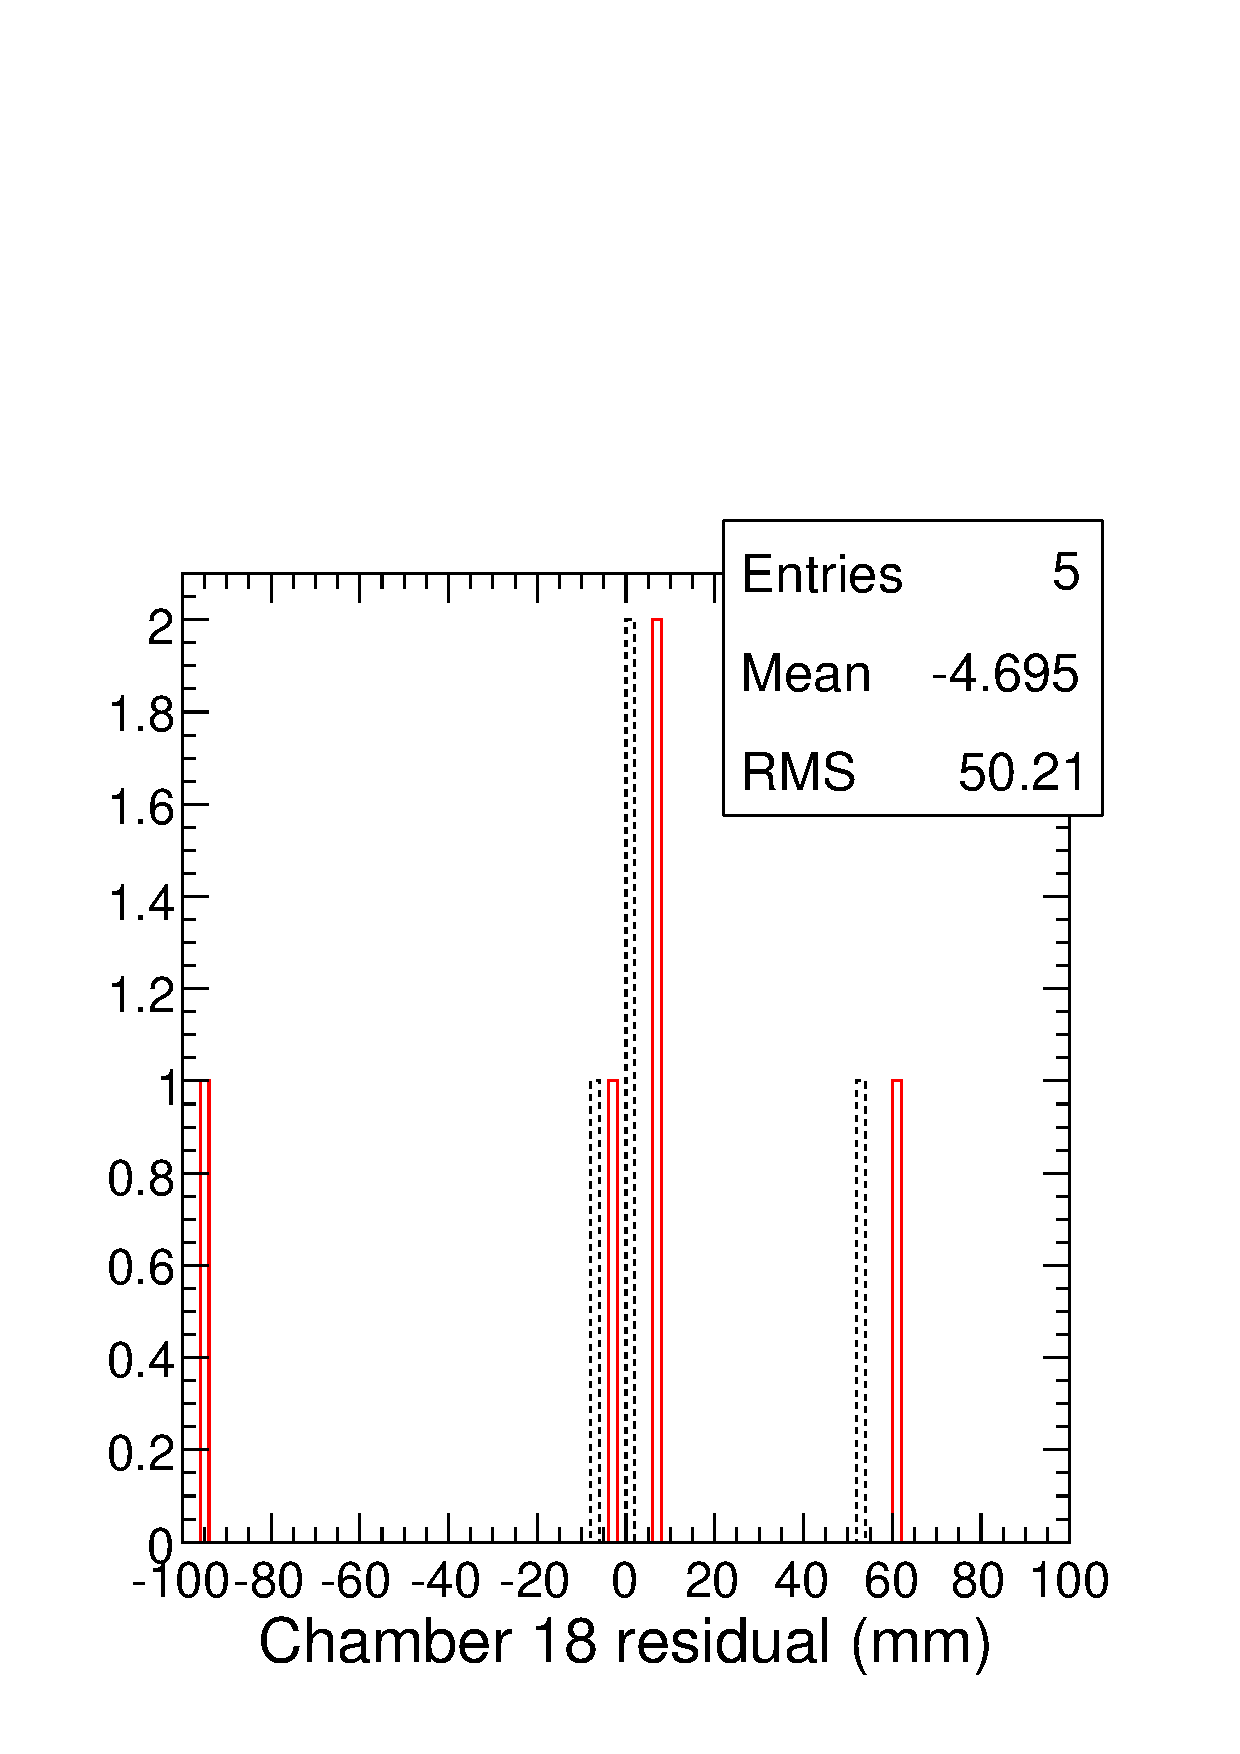
\includegraphics[width=0.11\linewidth]{endcap_mem22_18.pdf}

\includegraphics[width=0.11\linewidth]{endcap_mem22_19.pdf}
\includegraphics[width=0.11\linewidth]{endcap_mem22_20.pdf}
\includegraphics[width=0.11\linewidth]{endcap_mem22_21.pdf}
\includegraphics[width=0.11\linewidth]{endcap_mem22_22.pdf}
\includegraphics[width=0.11\linewidth]{endcap_mem22_23.pdf}
\includegraphics[width=0.11\linewidth]{endcap_mem22_24.pdf}
\includegraphics[width=0.11\linewidth]{endcap_mem22_25.pdf}
\includegraphics[width=0.11\linewidth]{endcap_mem22_26.pdf}
\includegraphics[width=0.11\linewidth]{endcap_mem22_27.pdf}

\includegraphics[width=0.11\linewidth]{endcap_mem22_28.pdf}
\includegraphics[width=0.11\linewidth]{endcap_mem22_29.pdf}
\includegraphics[width=0.11\linewidth]{endcap_mem22_30.pdf}
\includegraphics[width=0.11\linewidth]{endcap_mem22_31.pdf}
\includegraphics[width=0.11\linewidth]{endcap_mem22_32.pdf}
\includegraphics[width=0.11\linewidth]{endcap_mem22_33.pdf}
\includegraphics[width=0.11\linewidth]{endcap_mem22_34.pdf}
\includegraphics[width=0.11\linewidth]{endcap_mem22_35.pdf}
\includegraphics[width=0.11\linewidth]{endcap_mem22_36.pdf}

\end{frame}

\begin{frame}
\frametitle{Summary of constants}

\begin{itemize}\setlength{\itemsep}{0.2 cm}
\item Barrel alignment
\begin{itemize}\setlength{\itemsep}{0.1 cm}
\item DT internal alignment with tracks and checked by survey
\item global alignment relative to tracker checked by $1/p_T$ in cosmics splitting
\begin{itemize}\setlength{\itemsep}{0.1 cm}
\item aligned using $100 < p_T < 200$~GeV tracks
\item and the current tracker
\item current APEs negligibly affect results
\end{itemize}
\end{itemize}

{\tt \scriptsize /castor/cern.ch/user/p/pivarski/DTCRAFTiter03\_withCenteredTracker.db}

\item Endcap alignment
\begin{itemize}\setlength{\itemsep}{0.1 cm}
\item CSC photogrammetry at 0~T
\item SLM disk-bending measurements at 3.8~T
\item 3-DOF $\times$ 4 disk alignment with tracks
\end{itemize}

{\tt \scriptsize /castor/cern.ch/user/p/pivarski/CSCCRAFT\_HardwareAndPGAndDisk2.db}
\end{itemize}

\label{numpages}
\end{frame}

\end{document}
